\documentclass{mini}
\usepackage[utf8]{inputenc}
\usepackage{fancyvrb}
\usepackage{amsmath}
\usepackage{subfig}
\newcommand{\degree}{\ensuremath{^\circ}}
\newcommand{\hilight}[1]{\colorbox{yellow}{#1}}
\linespread{1.5}
\newcommand{\CMAES}{\mbox{CMA-ES}}
\DeclareUnicodeCharacter{00A0}{~}

%------------------------------------------------------------------------------%
\title{Analiza możliwości wykorzystania w~algorytmie CMA-ES wiedzy o~ograniczeniach kostkowych}

\author{inż. Robert Jakubowski}
\supervisor{dr hab. inż. Jarosław Arabas prof. nzw. PW}
\type{magisters}
\monthyear{Maj 2016}
\date{\today}
\album{237545}
%------------------------------------------------------------------------------%
\begin{document}

\maketitle

\pagebreak
\thispagestyle{empty}

\openup -0.2em %make it fit on one page
\tableofcontents
\openup 0.2em %make it fit on one page

\thispagestyle{empty}
\raggedbottom
\pagebreak


\section{Streszczenie}

\hspace{3,4ex}Niniejsza praca poświęcona jest badaniu wpływu różnych metod uwzględniania ograniczeń w algorytmie CMA-ES na jakość uzyskiwanych wyników optymalizacji.

We wstępie zaczynając od zarysowania kontekstu problemu przedstawiony został przedmiot badań i cel pracy. Cały rozdział można potraktować jako motywację do pracy.

Następnie opisano sam algorytm CMA-ES. Opisanie tego algorytmu jest niezbędne do zrozumienie jego mechanizmów, a w konsekwencji do przeprowadzenia badań. Zaczynając od przedstawienia pseudokodu, kolejne podrozdziały skupiają się na wyjaśnieniu istoty poszczególnych fragmentów algorytmu. 

W kolejnym rozdziale opisano techniki uwzględniania ograniczeń. Zawarto tam nie tylko opisy poszczególnych metod, ale również pokazano w sposób empiryczny jak mogą wpływać na algorytmy. W tym celu użyto algorytmu błądzenia przypadkowego. Zaimplementowano ten algorytm z różnymi wariantami uwzględniania ograniczeń, a następnie przeprowadzono szereg testów badających między innymi rozkłady prawdopodobieństw oraz wartości oczekiwanych.

Następny rozdział opisuje sposoby, w jaki mogą być testowane algorytmy optymalizacji globalnej. Niezbędne do testowania są specjalnie przygotowane zbiory funkcji benchmarkowych, które badają skuteczność algorytmów. W tej części przedstawiono również test Wilcoxona, który wykorzystuje się do porównania wyników funkcji benchmarkowych.

Opisane metody testowania zostały użyte w przedostatnim rozdziale, który przedstawia testy wykonane na algorytmie CMA-ES oraz jego modyfikacjach. Modyfikacje polegały wyłącznie na zmianie metod uwzględniania ograniczeń. Testy te mają na celu pokazanie zachowania algorytmu CMA-ES, gdy uruchamiana funkcja posiada ograniczenia oraz ukazanie, który wariant zwraca lepsze rezultaty. Wyniki tych testów zostały zebrane oraz omówione.

W ostatnim rozdziale podsumowane zostają wyniki pracy oraz wnioski z niej wynikające. Zaproponowane są również możliwe dalsze kierunki badań i rozwoju algorytmu CMA-ES mające poprawić jego działanie.

\subsubsection*{Słowa kluczowe}
CMA-ES, uwzględnianie ograniczeń, algorytmy ewolucyjne, ograniczenia kostkowe, optymalizacja

\pagebreak

\section{Abstract}
\hspace{3,4ex}This thesis discusses constraints methods in CMA-ES algorithm. It describes examination of various methods influence to quality of optimization results.

Introduction presents examinations target and subject. Whole chapter can be treated as thesis motivation.

The following chapter describes CMA-ES algorithm. This description is necessary to understand the algorithm and conduct examinations. While it starts with pseudocode, proceeding sections focus on explanation of main parts of algorithm.

In the next chapter constraints handling techniques are described. Besides methods description, their influence on algorithm results is presented. Random walk was used to achieve this goal. Random walk with various variants of constraints handling was implemented. After that there was conducted set of tests examinating probability distribution and expected value.

Subsequent chapter describes ways of global optimization algorithms testing. It is necessary to prepare particular collections of benchmark functions, which examines algorithms effectiveness. This part contains also introduction to Wilcoxon test, which is used for comparing benchmark functions results.

Described testing methods are used in penultimate chapter to present tests conducted on CMA-ES algorithm with modifications. This modifications depends only on change of constraints handling techniques. This tests goal is to show behaviour of CMA-ES algorithm when function has constraints. Moreover it should show which variant returns better outcomes. Results of tests are gathered and discussed.

The last chapter summarizes results of work and presents conclusions. Possibilities of another examinations and ideas for further improvement of CME-ES algorithm are provided at the end.

\subsubsection*{Keywords}
CMA-ES, constraints handling, evolutionary algorithm, box constraint, optimalization

\pagebreak

\section{Wstęp}
\hspace{3,4ex}Algorytmy ewolucyjne wykorzystuje się głównie w problemach poszukiwania optimum funkcji celu z wieloma zmiennymi, np. w planowaniu procesów przemysłowych.\cite{zast} W~większości algorytmów ewolucyjnych rozkład prawdopodobieństwa generowanych punktów nie zmienia się w trakcie symulacji algorytmu. Z~tego faktu wynika problem ustalenia parametrów początkowych, np. wariancji rozkładu prawdopodobieństwa generowanych punktów. Ustalenie zbyt niskiej wartości wariancji może prowadzić do znalezienia jedynie pewnego optimum lokalnego, natomiast ustalenie zbyt dużej wartości wariancji sprawia, że trudno znaleźć algorytmowi optimum globalne.

Naprzeciw problemowi ustalenia wariancji wychodzi algorytm CMA-ES. Już samo rozwinięcie akronimu CMA-ES mówi o tym: Covariance Matrix Adaptation - Evolution Strategy (strategia ewolucyjna z adaptacją macierzy kowariancji). Jest to algorytm oparty na technikach ewolucyjnych, aczkolwiek punkty losowane są na podstawie macierzy kowariancji (wielowymiarowe uogólnienie wariancji), która jest w każdej iteracji dostosowywana do aktualnej sytuacji przeszukiwań. Takie rozwiązanie sprawia, że dobór parametrów początkowych nie jest tak istotny jak w innych algorytmach ewolucyjnych.

Mimo kilkunastu lat istnienia algorytmu CMA-ES, podejmowane są kolejne próby jego optymalizacji (\cite{magist}\cite{lcmaes}). Warto jednocześnie pamiętać, że w większości wariantów algorytmu CMA-ES trudno mówić o uniwersalnej optymalizacji. Zazwyczaj poprawa w pewnej grupie funkcji skutkuje pogorszeniem wyników w innym rodzaju funkcji.

Ta praca zawiera badania, które mogą być pomocą podczas optymalizacji algorytmu CMA-ES skoncentrowanej na ograniczeniach kostkowych. Algorytm CMA-ES został stworzony głównie do problemów bez ograniczeń. Można go jednak stosować również do problemów z ograniczeniami, a w literaturze trudno znaleźć prace poświęcone temu zagadnieniu. Warto to zbadać, ponieważ ograniczenia napotykamy w wielu problemach - materiały mają wytrzymałość, komputery skończoną pamięć, a czasem ogranicza prędkość światła.

W aktualnej wersji algorytmu CMA-ES punkty, które znajdą się poza ograniczeniem, są na to ograniczenie rzutowane (o rzutowaniu można przeczytać w rozdziale \ref{secrzut}). Jest to tylko jedna z metod uwzględniania ograniczeń. Warto zauważyć, że zamiast rzutować punkt na ograniczenie, można go reinicjować, powtórnie losować, czy też przekształcić symetrycznie względem ograniczeń, co omówiono dokładniej w rozdziale \ref{technikiogr}.

\subsection*{Cel pracy}
\hspace{3,4ex}Celem pracy jest weryfikacja wpływu uwzględniania ograniczeń na algorytm \CMAES. Zbadanych będzie kilka metod uwzględniania ograniczeń. Cel będzie realizowany poprzez analizę eksperymentalną.

\pagebreak

\section{Algorytm CMA-ES} \label{secalgcmaes}
\hspace{3,4ex}Zgodnie z tym, co zostało ustalone we wstępie, algorytm CMA-ES należy do rodziny algorytmów ewolucyjnych. Cechą wyróżniającą ten algorytm jest specyficzny sposób generowania punktów. Można to zauważyć w poniższym pseudokodzie opisującym algorytm CMA-ES (równania są cytowaniami z \cite{cmaes_tutorial}):
\begin{Verbatim}
inicjuj zmienne
dopóki nie są spełnione warunki stopu:
	generuj punkty
\end{Verbatim}
(1)\hspace{12ex} $x_k^{t+1} \sim m^t + \sigma^tN(0,C^t)$
\begin{Verbatim}
	oblicz wartości funkcji celu w wygenerowanych punktach
	posortuj punkty
\end{Verbatim}
(2)\hspace{12ex} $f(x_{1:\lambda}^{t+1}) \leq f(x_{2:\lambda}^{t+1}) \leq ... \leq f(x_{\lambda:\lambda}^{t+1})$
\begin{Verbatim}
	przeprowadź selekcję punktów
	oblicz wartość oczekiwaną rozkładu
\end{Verbatim}
(3)\hspace{12ex} $m^{t+1}=m^t+c_m\sum\limits_{i=1}^\mu w_i(x_{i:\lambda}^{t+1}-m^t)$
\begin{Verbatim}
	oblicz długość kroku
\end{Verbatim}
(4)\hspace{12ex} $p_\sigma^{t+1}=(1-c_\sigma)p_\sigma^t+\sqrt{c_\sigma(2-c_\sigma)\mu_{eff}}{C^t}^{-\frac{1}{2}}\frac{m^{t+1}-m^t}{\sigma^t}$ \\
(5)\hspace{12ex} $\sigma^{t+1}=\sigma^t exp (\frac{c_\sigma}{d_\sigma}(\frac{\|p_\sigma^{t+1}\|}{E\|N(0,I)\|}-1))$
\begin{Verbatim}
	oblicz macierz kowariancji
\end{Verbatim}
(6)\hspace{12ex} $p_c^{t+1} = (1-c_c)p_c^t+\sqrt{c_c(2-c_c)\mu_{eff}}\frac{m^{t+1}-m^t}{\sigma^t}$ \\
(7)\hspace{12ex} $C^{t+1} = (1-c_1-c_\mu\sum\limits_{j=1}^\lambda w_j)C^t+c_1p_c^{t+1}{(p_c^{t+1})}^T+c_\mu \sum\limits_{i=1}^\lambda w_iy_{i:\lambda}^{t+1}{(y_{i:\lambda}^{t+1})}^T$
\newline
gdzie:
\begin{itemize}[noitemsep]
\item $x_k^t$ - k-ty punkt iteracji numer t
\item $m^t$ - wartość oczekiwana rozkładu w iteracji t
\item $\sigma^t$ - długość kroku iteracji t
\item $N(p,C)$ - losowanie punktu z rozkładem normalnym o wartości oczekiwanej w~punkcie p oraz macierzy kowariancji C
\item $C^t$ - macierz kowariancji iteracji t
\item $f(x)$ - wartość funkcji celu w punkcie x
\item $\lambda$ - wielkość populacji (ilość punktów x w jednej iteracji)
\item $c_m$ - współczynnik nauki wartości oczekiwanej
\item $\mu$ - liczba wybieranych punktów spośród wszystkich $\lambda$ punktów (patrz \ref{selekcjapunktow} Selekcja punktów)
\item $w_i$ - waga punktu $x_i$
\item $p_\sigma^t$ - sprzężona ścieżka ewolucji w iteracji t
\item $c_\sigma$ - współczynnik nauki długości kroku
\item $\mu_{eff}=\frac{1}{\sum\limits_{i=1}^\mu w_i^2}$
\item $d_\sigma \approx 1$ - stała tłumienia
\item $p_c^t$ - ścieżka ewolucji w iteracji t
\item $c_c$ - współczynnik nauki macierzy kowariancji
\item $c_1 \approx \frac{2}{n^2}$
\item $c_\mu \approx min(\frac{\mu_{eff}}{n^2}, 1-c_1)$
\item $y_{i:\lambda}^{t+1} = \frac{x_{i:\lambda}^{t+1}-m^t}{\sigma^t}$
\end{itemize}

Najważniejsze części algorytmu są opisane poniżej w następującej kolejności: macierz kowariancji, wartość oczekiwana rozkładu, długość kroku, generowanie punktów, selekcja punktów.

\subsection{Macierz kowariancji} \label{macierz}
\hspace{3,4ex}Punkty w algorytmie CMA-ES są generowanie poprzez losowanie na podstawie macierzy kowariancji $C^t$ zgodnie ze wzorem (1). Oznacza to, że nie istnieje bezpośredni związek pomiędzy punktami kolejnych iteracji - w~klasycznych algorytmach ewolucyjnych zazwyczaj można było mówić o rodzicach wygenerowanego punktu. Punkty wpływają jednak na macierz kowariancji, a pośrednio przez nią na kolejną generację punktów. Odbywa się to w~następujący sposób: spośród wszystkich punktów wybiera się $\mu$ punktów (zazwyczaj połowę), która zwraca lepsze wartości funkcji celu. Następnie przypisuje się im wagi $w$ - w~zależności od tego, jak dobry jest punkt. Na postawie tych danych wyznaczana jest empiryczna macierz kowariancji (6-7).

\subsection{Wartość oczekiwana rozkładu} \label{wartoscoczekiwana}
\hspace{3,4ex}Punkty generowane są na podstawie rozkładu określonego macierzą kowariancji. Sama macierz nie mówi jednak nic o wartości oczekiwanej. Wymaga to oddzielnego wyznaczenia tej wartości(3).

Podobnie jak w przypadku macierzy kowariancji, wybiera się $\mu$ punktów. Dla tych punktów wyznaczane są wektory przesunięć względem wartości oczekiwanej (każdy wektor jest skalowany przez wagę punktu). Wektory te sumujemy otrzymując pewien wektor wynikowy, który następnie jeszcze skalujemy przez współczynnik nauki $c_m$. O~tak otrzymany wektor przesuwamy dotychczasową wartość oczekiwaną.

\subsection{Długość kroku}
\hspace{3,4ex}Generowanie punktów z macierzy kowariancji pozwala na skalowanie tego rozkładu poprzez użycie dodatkowego parametru $\sigma^t$. Ten parametr jest nazywany długością kroku. W~algorytmie CMA-ES długość kroku obliczana jest na podstawie kierunku przemieszczania się wartości oczekiwanej rozkładu. Długość kroku zwiększa się, gdy wartość oczekiwana przemieszcza się w tym samym kierunku. Skraca się ona natomiast, gdy kierunek jest zmienny.

\subsection{Selekcja punktów} \label{selekcjapunktow}
\hspace{3,4ex}Selekcja punktów, to wybór $\mu$ punktów spośród całej populacji. Wybierane są te punkty, które mają lepszą wartość funkcji (2). Wartość funkcji wpływa również na przypisywane punktom wagi, o których wspomniano wcześniej.

\subsection{Ocena algorytmu}
\hspace{3,4ex}Powyższe opisy pokazują, że algorytm CMA-ES posiada wiele zmiennych i parametrów. Zmienne, takie jak macierz kowariancji czy długość kroku, są wyznaczane na podstawie rozbudowanych równań. W tym miejscu powstaje pytanie, czy warto zajmować się takim algorytmem, gdy istnieją rozwiązania o przejrzystej strukturze. Odpowiedzią niech będą wyniki badań \cite{bbob}, które pokazują, że dla skomplikowanych funkcji algorytm CMA-ES zwraca bardzo dobre rezultaty.

\pagebreak

\section{Techniki uwzględniania ograniczeń} \label{technikiogr}
\hspace{3,4ex}Niektóre problemy optymalizacyjne posiadają ograniczenia. Szukając rozwiązania należy zapewnić, że będzie ono dopuszczalne. Bazując na \cite{wyklady} techniki uwzględniania ograniczeń można podzielić ze względu na wykorzystanie:
\begin{itemize}[noitemsep]
\item definicji przestrzeni przeszukiwań - zapewnienie, że podczas krzyżowań, mutacji i innych zmian punktów, żaden z punktów nie wypadnie poza przestrzeń przeszukiwań,
\item modyfikacji funkcji celu - zmienienie funkcji celu tak, aby funkcja celu dla punktów spoza ograniczeń zwracały gorsze wyniki,
\item transformacji rozwiązań - punkty, które są poza ograniczeniami zostają zamieniane na punkty, które znajdują się w ograniczeniach.
\end{itemize}

Każda z tych technik posiada wiele wariantów. Przeanalizowanie wszystkich mogłoby być bardzo czasochłonne. W związku z tym w tej pracy skupiono się na transformacji rozwiązań.

Ograniczenia w problemach mogą różnić się ze względu na swój charakter, np. mogą być nieciągłe lub punktowe. Niniejsza praca skupia się na ograniczeniach kostkowych.

\subsection{Transformacje rozwiązań} \label{transformacje}
\hspace{3,4ex}Istnieje wiele technik transformacji rozwiązań. W~kolejnych podrozdziałach znajdują się metody transformacji, które były badane na potrzeby tej pracy. Każda z technik jest opisana słownie oraz pseudokodem. Opis słowny zawiera wyjaśnienie, co się dzieje z punktem, który znalazł się poza ograniczeniem. W~pseudokodzie zastosowano następujące oznaczenia:
\begin{itemize}[noitemsep]
\item $x$ - punkt, który poddajemy naprawie
\item $y$ - punkt, który powstał po naprawie punktu $x$
\item $x'$ - rodzic punktu $x$; z punktu $x'$ z zadanym rozkładem został wygenerowany punkt $x$
\item $x(i)$ - wartość $i$-tej współrzędnej punktu $x$
\item $lb$ - ograniczenie dolne
\item $ub$ - ograniczenie górne
\end{itemize}

\subsubsection{Metoda konserwatywna}
\hspace{3,4ex}Nowy punkt zostaje odrzucony i wraca do poprzedniej pozycji.

\begin{Verbatim}[baselinestretch=1.1]
y = x'
\end{Verbatim}


\subsubsection{Rzutowanie} \label{secrzut}
\hspace{3,4ex}Punkt jest transformowany do najbliższego punktu, który spełnia ograniczenia kostkowe. Oznacza to, że dla każdej współrzędnej sprawdzany jest warunek zawierania się w~ograniczeniach. Wartości współrzędnych, dla których nie jest on spełniony, zmieniane są na wartości ograniczeń (odpowiednio dolne lub górne), które są najbliżej.

\begin{Verbatim}[baselinestretch=1.1]
dla każdej współrzędnej i
	jeżeli lb(i) > x(i)
		y(i) = lb(i)
	jeżeli ub(i) < x(i)
		y(i) = ub(i)
	jeżeli lb(i) <= x(i) <= ub(i)
		y(i) = x(i)
\end{Verbatim}

\subsubsection{Reinicjacja} \label{reinicjacja}
\hspace{3,4ex}Punkt jest przenoszony do ustalonej pozycji - często jest to punkt początkowy.

\begin{Verbatim}[baselinestretch=1.1]
y = xr
\end{Verbatim}

\subsubsection{Powtórna generacja}
\hspace{3,4ex}Punkt jest powtórnie generowany do momentu, aż spełni ograniczenie.

\begin{Verbatim}[baselinestretch=1.1]
dopóki !w_ograniczeniach(x)
	x = generuj(x')
y=x
\end{Verbatim}

\subsubsection{Zawijanie}
\hspace{3,4ex}Dla każdej współrzędnej sprawdzane są warunki ograniczeń. W przypadku współrzędnych, na których punkt jest poza ograniczeniem, różnica pomiędzy ograniczeniem a~wartością współrzędnej punktu jest zapamiętywana. Tę różnicę odkładamy na przeciwległym ograniczeniu po stronie, która jest wewnątrz ograniczeń. W tym miejscu znajduje się nowa wartość współrzędnej punktu. Z perspektywy punktu nie ma ograniczeń, a przestrzeń przeszukiwań po każdym wymiarze jest jakby "zawinięta".

\begin{Verbatim}[baselinestretch=1.1]
dla każdej współrzędnej i
	jeżeli lb(i) > x(i)
		y(i) = ub(i) - (lb(i) - x(i))
	jeżeli ub(i) < x(i)
		y(i) = lb(i) + (x(i) - ub(i))
	jeżeli lb(i) <= x(i) <= ub(i)
		y(i) = x(i)
\end{Verbatim}

\subsubsection{Odbicie}
\hspace{3,4ex}Dla każdej współrzędnej sprawdzane są warunki ograniczeń. W przypadku współrzędnych, na których punkt jest poza ograniczeniem, wartość punktu tej współrzędnej jest symetrycznie odbita względem ograniczenia, którego warunek został złamany.

\begin{Verbatim}[baselinestretch=1.1]
dla każdej współrzędnej i
	jeżeli lb(i) > x(i)
		y(i) = x(i) + 2 * (lb(i) - x(i))
	jeżeli ub(i) < x(i)
		y(i) = x(i) - 2 * (x(i) - ub(i))
	jeżeli lb(i) <= x(i) <= ub(i)
		y(i) = x(i)
\end{Verbatim}

\subsection{Błądzenie przypadkowe} \label{bladzenie}
\hspace{3,4ex}Na podstawie pseudokodu zawartego w rozdziale \ref{secalgcmaes} (szczególnie równań 4-5) można się spodziewać, że algorytm CMA-ES dla funkcji stałej będzie zachowywał się analogicznie do błądzenia przypadkowego. Przekonanie takie jest częstokroć wypowiadane ustnie przez N. Hansena, twórcę metody. Takie założenie skłoniło autora, żeby zbadać błądzenie przypadkowe z ograniczeniami. Błądzenie przypadkowe jest algorytmem prostszym niż CMA-ES, więc umożliwia szybsze testowanie i wyciąganie wniosków.

Niech $ X_1, X_2, ... $ będą realizacjami niezależnych n-wymiarowych zmiennych losowych o wartości oczekiwanej równej $ [0]^n $. Błądzenie przypadkowe, to proces generujący sekwencję punktów $S_1$, $S_2$, ..., takich że:

\begin{equation}
S_1 = X_1, S_i=S_{i-1}+X_i
\end{equation}

Zmienne losowe mogą być realizowane w różny sposób. Mogą to być wektory o~rozkładzie normalnym, jednostajnym lub innym.

\subsection{Metoda przeprowadzania testów}
\hspace{3,4ex}Celem testów jest zaobserwowanie, jaki wpływ na symulację błądzenia przypadkowego ma metoda uwzględniania ograniczeń. Do tak postawionego celu można podejść na różne sposoby. Wybrano dwie cechy, których analiza powinna przyczynić się do realizacji postawionego celu. Są nimi:
\begin{enumerate}
\item Wartość oczekiwana generowanego punktu (razem z poprawą).
\item Rozkład prawdopodobieństwa generowanych punktów.
\end{enumerate}

Sposoby testowania obu cech są opisane w kolejnych podrozdziałach.

\subsubsection{Wartość oczekiwana generowanego punktu}
\hspace{3,4ex}Wartością oczekiwaną zmiennej losowej w błądzeniu przypadkowym jest $[0]^n$. Implikuje to fakt, że wartością oczekiwaną $S_i$ jest $S_{i-1}$. Ustalenie ograniczeń kostkowych nie zmienia faktu, że nadal losowany jest wektor $X_i$, którego wartość oczekiwana jest równa $[0]^n$. Dodajemy jednak metody naprawy. W związku z tym wartością oczekiwaną $S_i$ nie zawsze jest $S_{i-1}$.

Dla każdego punktu $p$ przestrzeni przeszukiwań można przypisać pewien wektor $\overrightarrow{d}$. Początek $\overrightarrow{d}$ znajduje się w $p$. Załóżmy teraz, że $p$ jest punktem $S_i$ pewnego błądzenia przypadkowego z ograniczeniami. Koniec wektora $\overrightarrow{d}$ znajduje się w wartości oczekiwanej punktu $S_{i+1}$.

Wykres, który będzie zawierał wektory $\overrightarrow{d}$, pozwoli na określenie charakterystyki przemieszczania się punktów w poszczególnych częściach przestrzeni przeszukiwań.

\subsubsection*{Implementacja}
\hspace{3,4ex}Do wizualizacji wybrano symulację, w której punkty pochodzą z przestrzeni dwuwymiarowej. Pozwala to na przejrzystą wizualizację wektorów $\overrightarrow{d}$ oraz pokazuje zachowanie wektorów, które są blisko kilku ograniczeń.

Do symulacji wybrano punkty równomiernie rozłożone na prostokątnej siatce dwuwymiarowej. Dla każdego z tych punktów przeprowadzono następujące obliczenia. 1000 razy uruchomiono symulację jednego kroku algorytmu błądzenia przypadkowego (z~rozkładem normalnym o wariancji równej 1 na obu wymiarach) z odpowiednią naprawą. Otrzymano tysiąc punktów, z których następnie obliczono średnią arytmetyczną. Tak uzyskany punkt potraktowano jako wartość oczekiwaną i wyrysowano wektor $\overrightarrow{d}$.

\subsubsection{Rozkład punktów wygenerowanych za pomocą błądzenia przypadkowego}
\hspace{3,4ex}Punkty w błądzeniu przypadkowym poruszają się chaotycznie. Ta losowość jest częściowo uporządkowana na ograniczeniach. W zależności od metody naprawy, punkty zachowują się inaczej, a rozkład prawdopodobieństwa jest zniekształcony. Autor postanowił przyjrzeć się jak wygląda rozkład prawdopodobieństwa wystąpienia punktu z~perspektywy całej symulacji.

Dla każdej metody naprawy opisanej w \ref{transformacje} jednokrotnie uruchomiono algorytm błądzenia przypadkowego z rozkładem normalnym z wariancją równą 0.5. Dodatkowo analizowano również błądzenie przypadkowe z rozkładem jednostajnym na przedziale $[-0.5; 0.5]$ (przedział co najmniej kilkukrotnie krótszy od ograniczeń kostkowych). Po każdej iteracji nowo wygenerowany punkt zapisywano w tablicy. Z tak przygotowanej tablicy generowano histogram.

\subsubsection*{Implementacja}
\hspace{3,4ex}Dla każdej z metod naprawy przygotowano oddzielny skrypt. Pseudokod skryptu zamieszczono poniżej.
\begin{Verbatim}[baselinestretch=1.1]
x - błądzący punkt
punkty - tablica wszystkich położeń punktu x
iteracje - liczba iteracji podana jako parametr
i = 0
dopóki i < iteracje
	d = wektor wylosowany z zadanym rozkładem
	x = x + d
	jeżeli x jest poza ograniczeniem
		popraw x
	dodaj x do tablicy punktów
	i = i + 1
\end{Verbatim}

\subsection{Wyniki testów}
\hspace{3,4ex}Wykresy zamieszczone w tym podrozdziale są dwóch rodzajów. Są to wykresy wektorów $\overrightarrow{d}$ przesunięć wartości oczekiwanych oraz histogramy wystąpień punktu.

Histogramy były tworzone poprzez symulacje skryptów z liczbą iteracji wynoszącą od 2 do 100 milionów. Szerokość przedziałów jest różna i była dobierana tak, aby jak najlepiej przedstawić interesujące fakty. Wszystkie wykresy, które pokazują wyniki błądzenia przypadkowego w dwóch wymiarach zostały przetworzone w następujący sposób: otrzymane wyniki symulacji powielono poprzez symetryczne odbicie ich względem osi X, osi Y oraz początku układu współrzędnych. Wykonano ten zabieg, aby zwiększyć dokładność wyników. Nie wpływają one na badania, ponieważ punkty 0 są środkami ograniczeń obu osi, a z perspektywy algorytmu nie ma znaczenia, w której ćwiartce znajduje się aktualnie punkt.

\subsubsection*{Metoda konserwatywna}
\hspace{3,4ex}Wektory wartości oczekiwanych, które są blisko ograniczeń są skierowane od ograniczenia. Histogramy z kolei pokazują, że punkty z większym prawdopodobieństwem występują przy ograniczeniach. Takie zachowanie wynika z tego, że potomkowie punktów blisko granicy mogą "wypaść" poza ograniczenie. Po naprawie dziecko będzie tym samym punktem.

\begin{figure}[H]
\centering
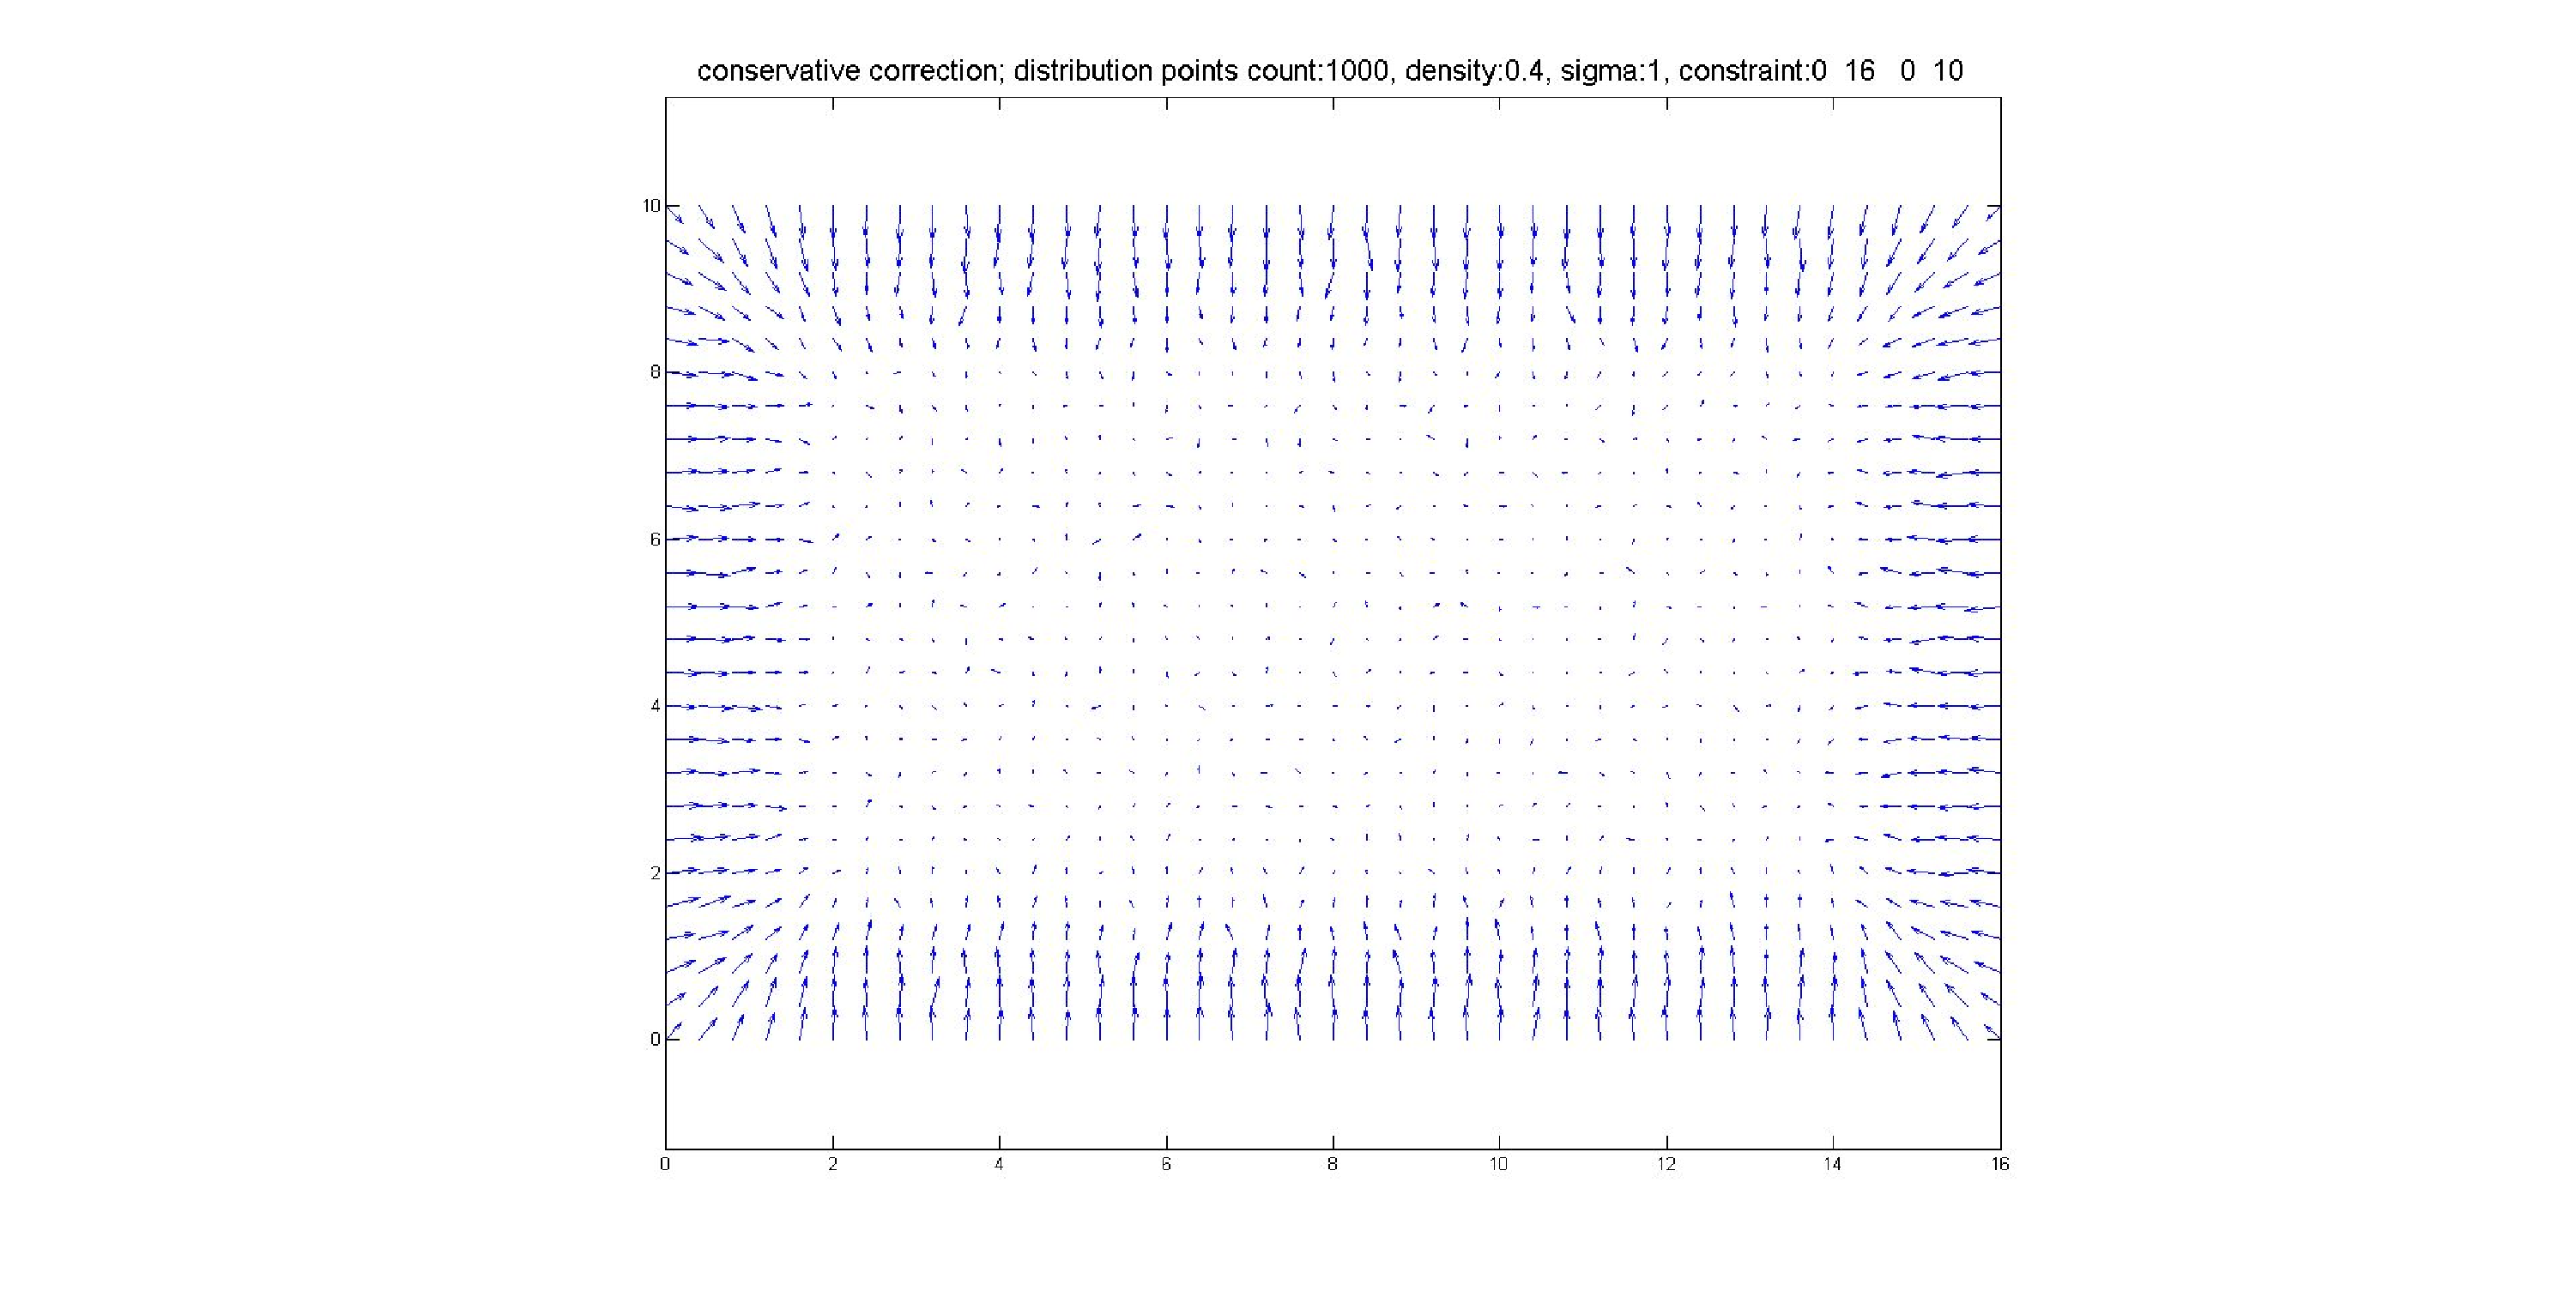
\includegraphics[width=\textwidth]{conservative2dprzesuniecie}
\caption{Wykres wektorów przesunięć wartości oczekiwanych dla konserwatywnej metody naprawy}
\end{figure}

\begin{figure}[H]
\centering
\subfloat[Generowanie z rozkładem normalnym]{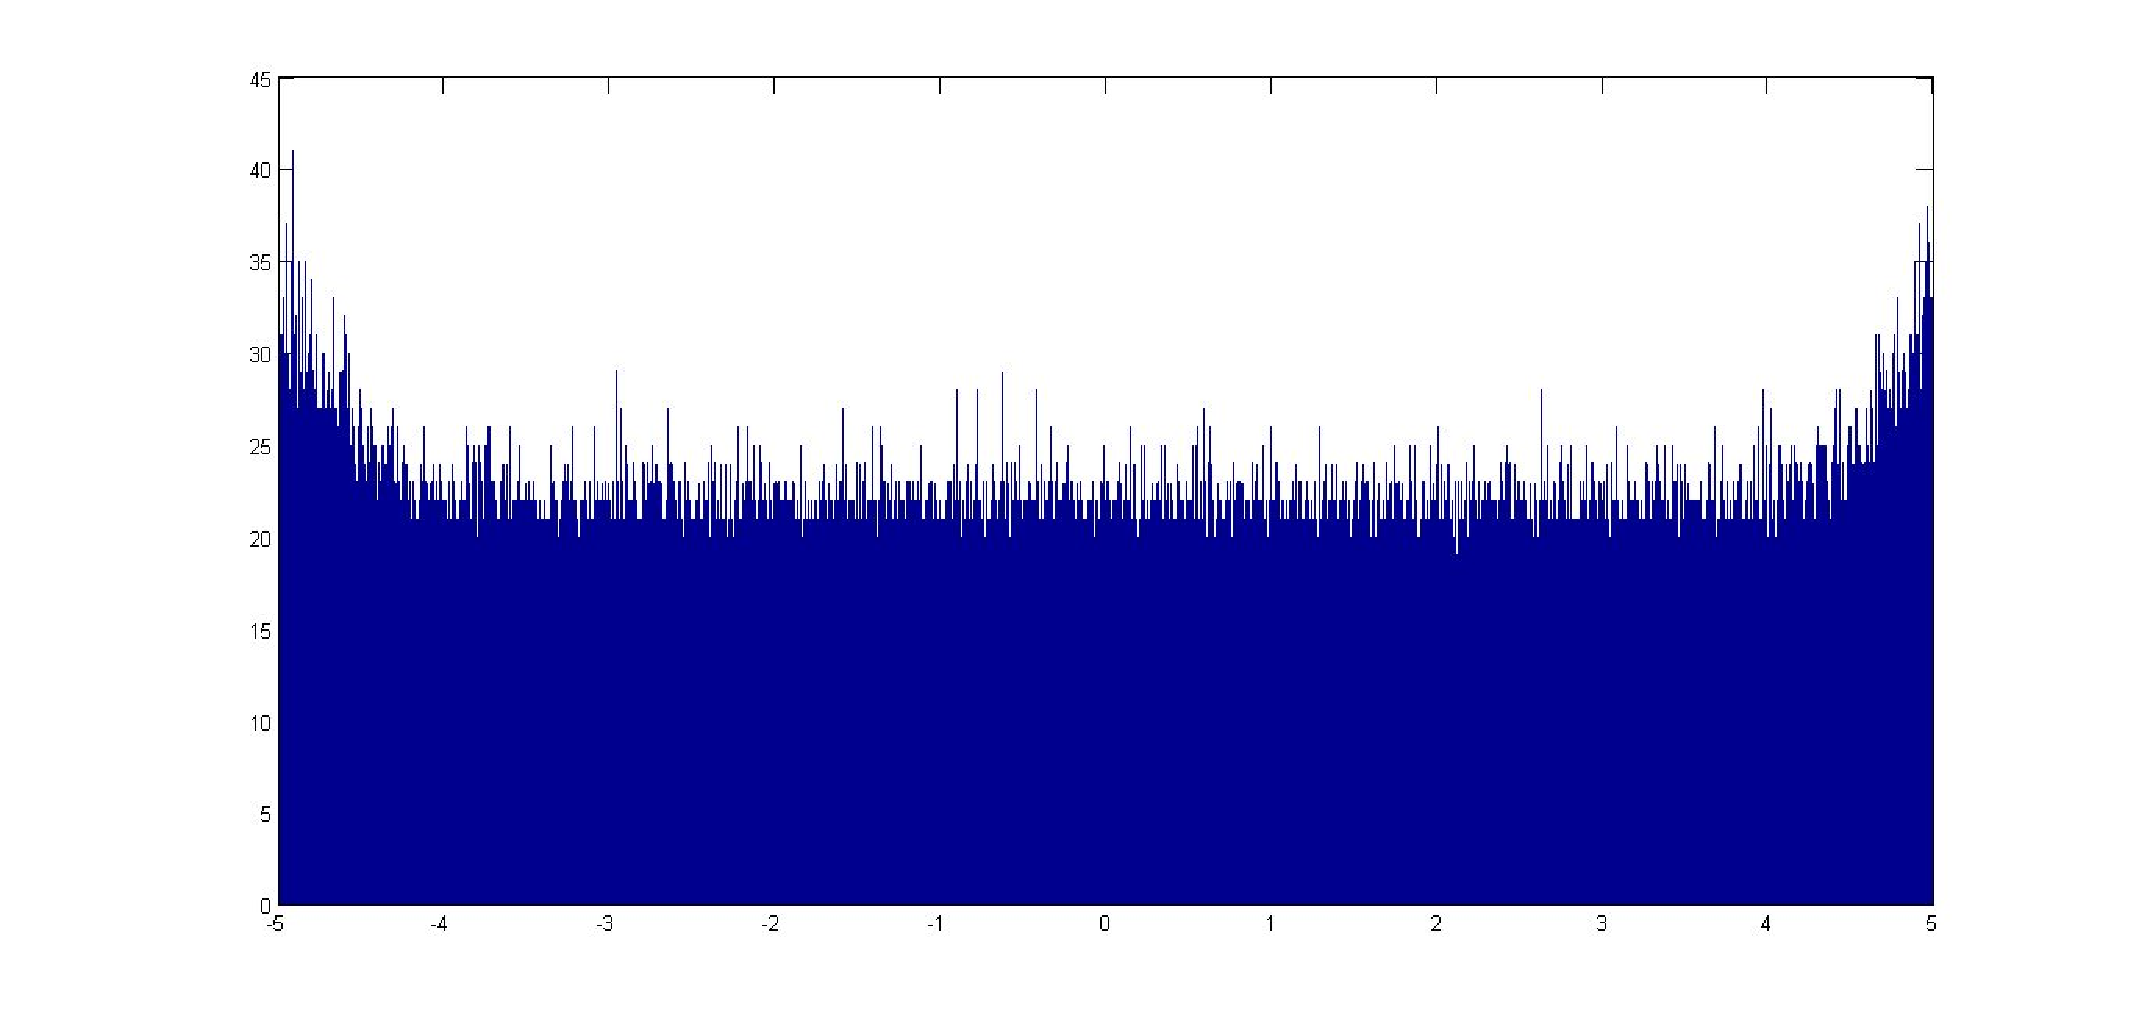
\includegraphics[width=0.45\textwidth]{c_n_20M_1__5_5_2}}
\quad
\subfloat[Generowanie z rozkładem jednostajnym]{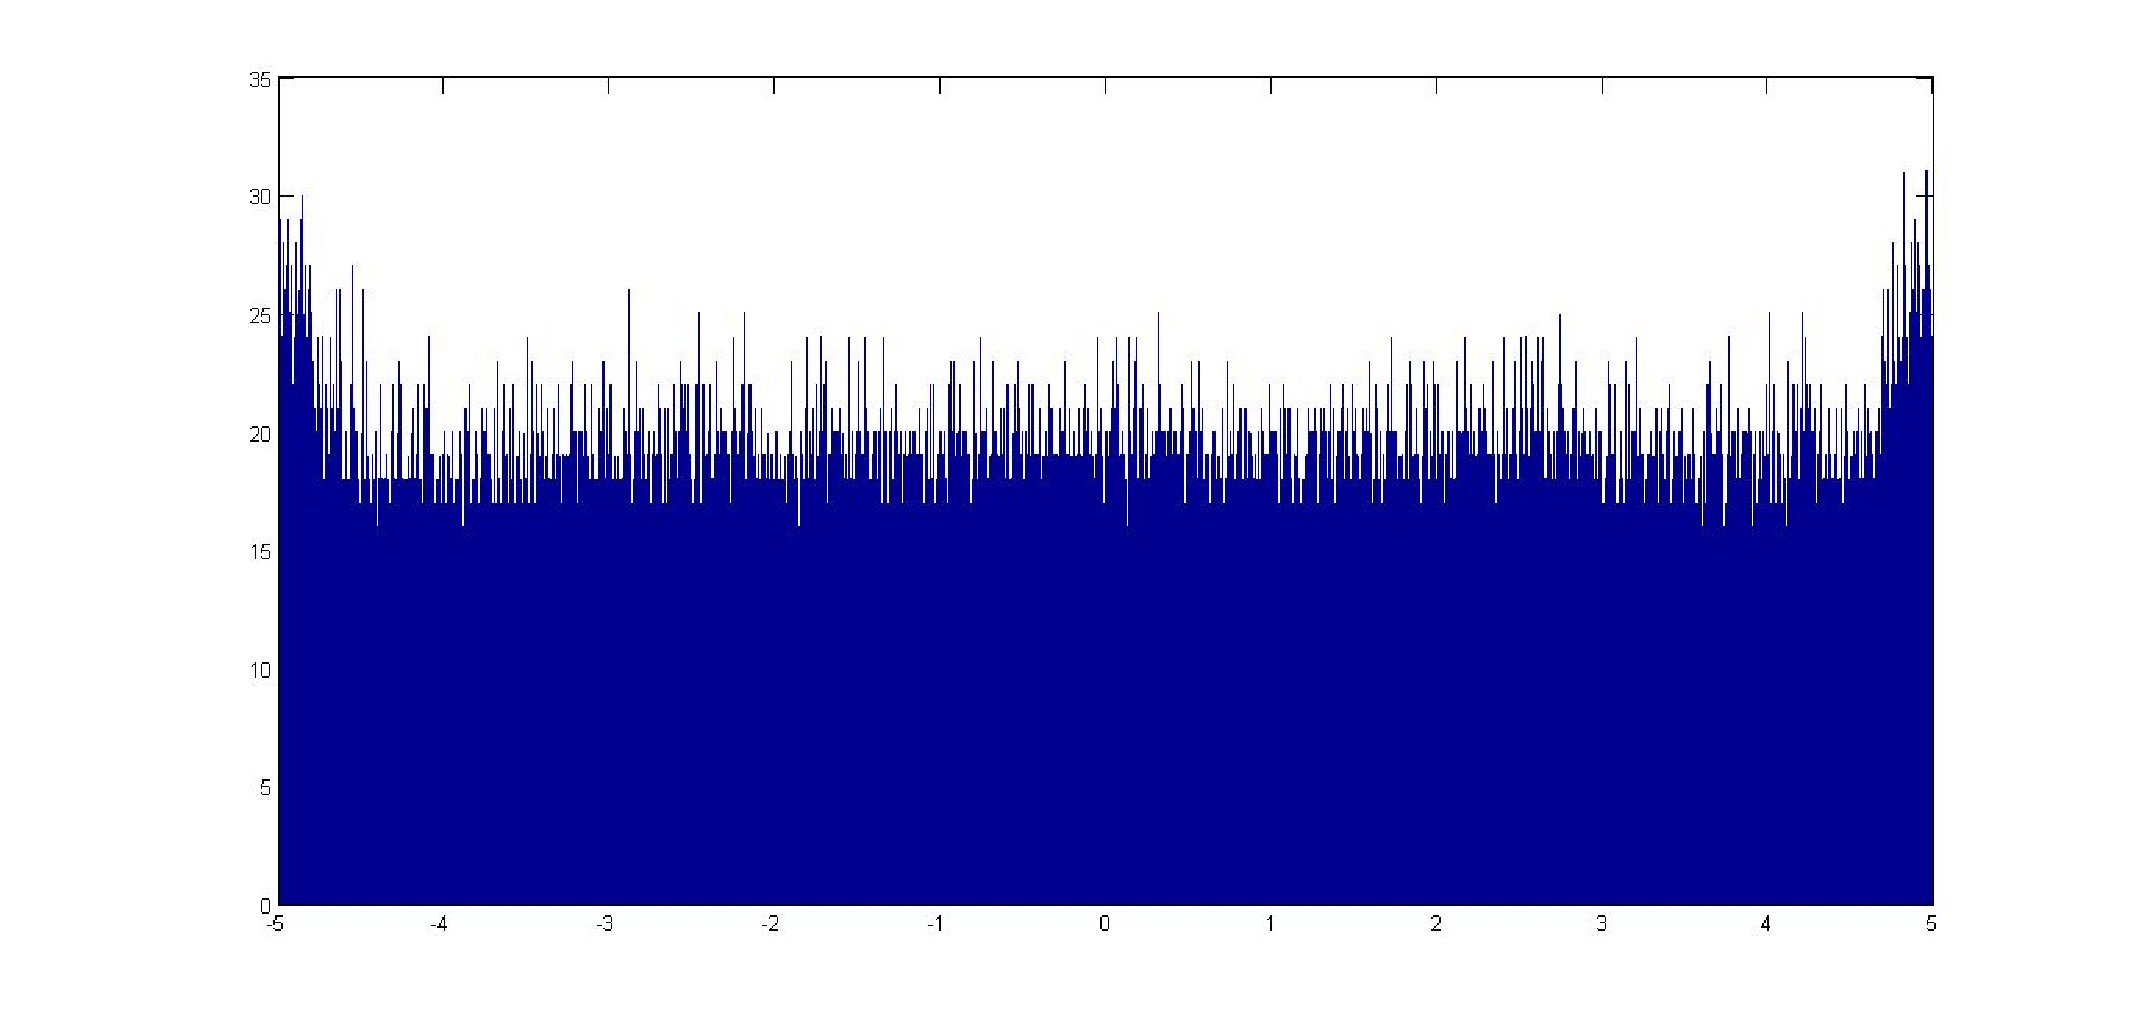
\includegraphics[width=0.45\textwidth]{c_j_2M_1__5_5}}
\caption{Histogram wystąpień punktów; konserwatywna metoda naprawy; 1~wymiar}
\end{figure}

\begin{figure}[H]
\centering
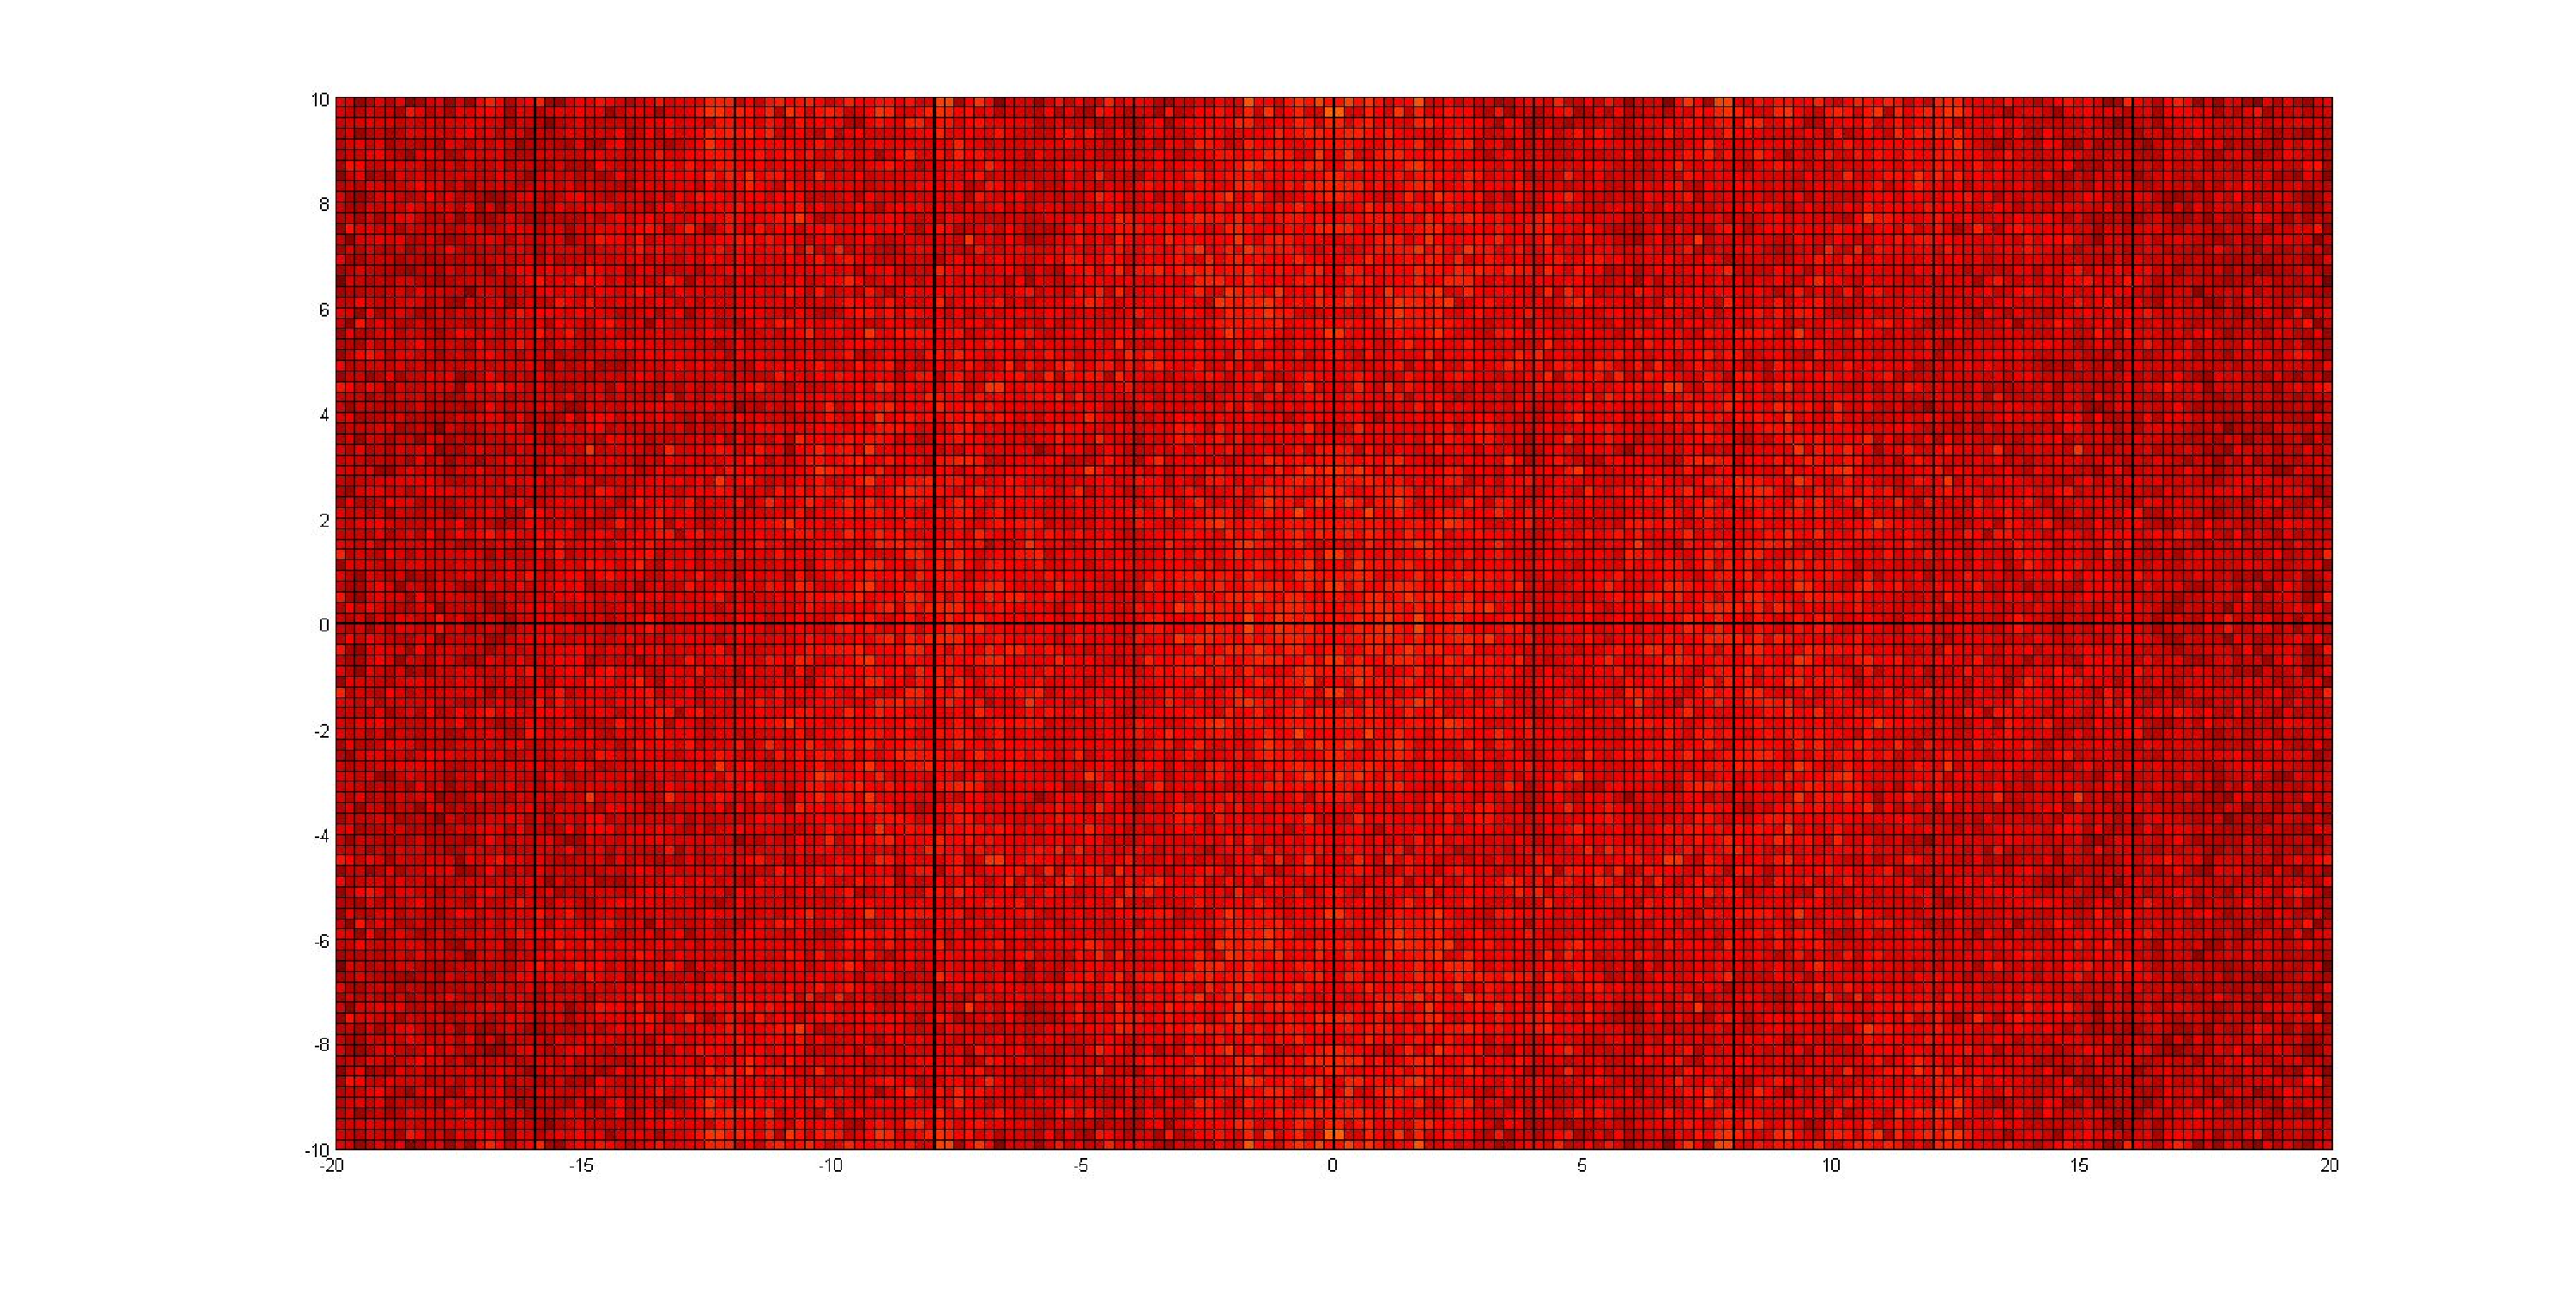
\includegraphics[width=\textwidth]{c_n_10M_2__20_20__10_10_4}
\caption{Histogram wystąpień punktów; konserwatywna metoda naprawy; 2 wymiary; generowanie z rozkładem normalnym}
\end{figure}

\subsubsection*{Rzutowanie}
\hspace{3,4ex}Zgodnie z przewidywaniami największe prawdopodobieństwo wystąpienia punktu jest na ograniczeniu, co bardzo dobrze obrazuje rysunek \ref{bladzenie:rzutowanie2d}. Na rysunkach \ref{bladzenie:rzutowanie1dn} i \ref{bladzenie:rzutowanie1dj} zakres osi~Y został zmniejszony do odpowiednio $[30000;60000]$ oraz $[70000;140000]$, aby uwypuklić interesujące efekty. W związku z tym, wartości przedziałów brzegowych nie są widoczne - były o kilka rzędów wielkości większe od pozostałych wartości.

Warto zwrócić uwagę na niespodziewane zjawisko - wartości dla przedziałów znajdujących się blisko ograniczeń są mniejsze niż pozostałe. Oznacza to, że punkty w tych przedziałach występują z mniejszym prawdopodobieństwem niż pozostałe. Wydawać by się mogło, że powinno być inaczej, ponieważ podczas symulacji punkty często są rzutowane na ograniczenie. Dodatkowo, w rozkładzie jednostajnym widać, że istnieją przedziały, w~których punkty występują z~większym prawdopodobieństwem. Autorowi nie udało się formalnie uzasadnić tego zjawiska. Intuicja prowadzi do hipotezy, że punkty, które znalazły się poza ograniczeniem, bez naprawy po kilku iteracjach zapełniałyby "dołek". Naprawa natomiast sprawia, że cała dalsza symulacja zostaje niejako przesunięta. W~ten sposób powstaje "górka" w~rozkładzie jednostajnym. Brak górki w rozkładzie normalnym można tłumaczyć charakterystyką samego rozkładu - spadek prawdopodobieństwa wraz z~oddalaniem się od wartości oczekiwanej.

\begin{figure}[H]
\centering
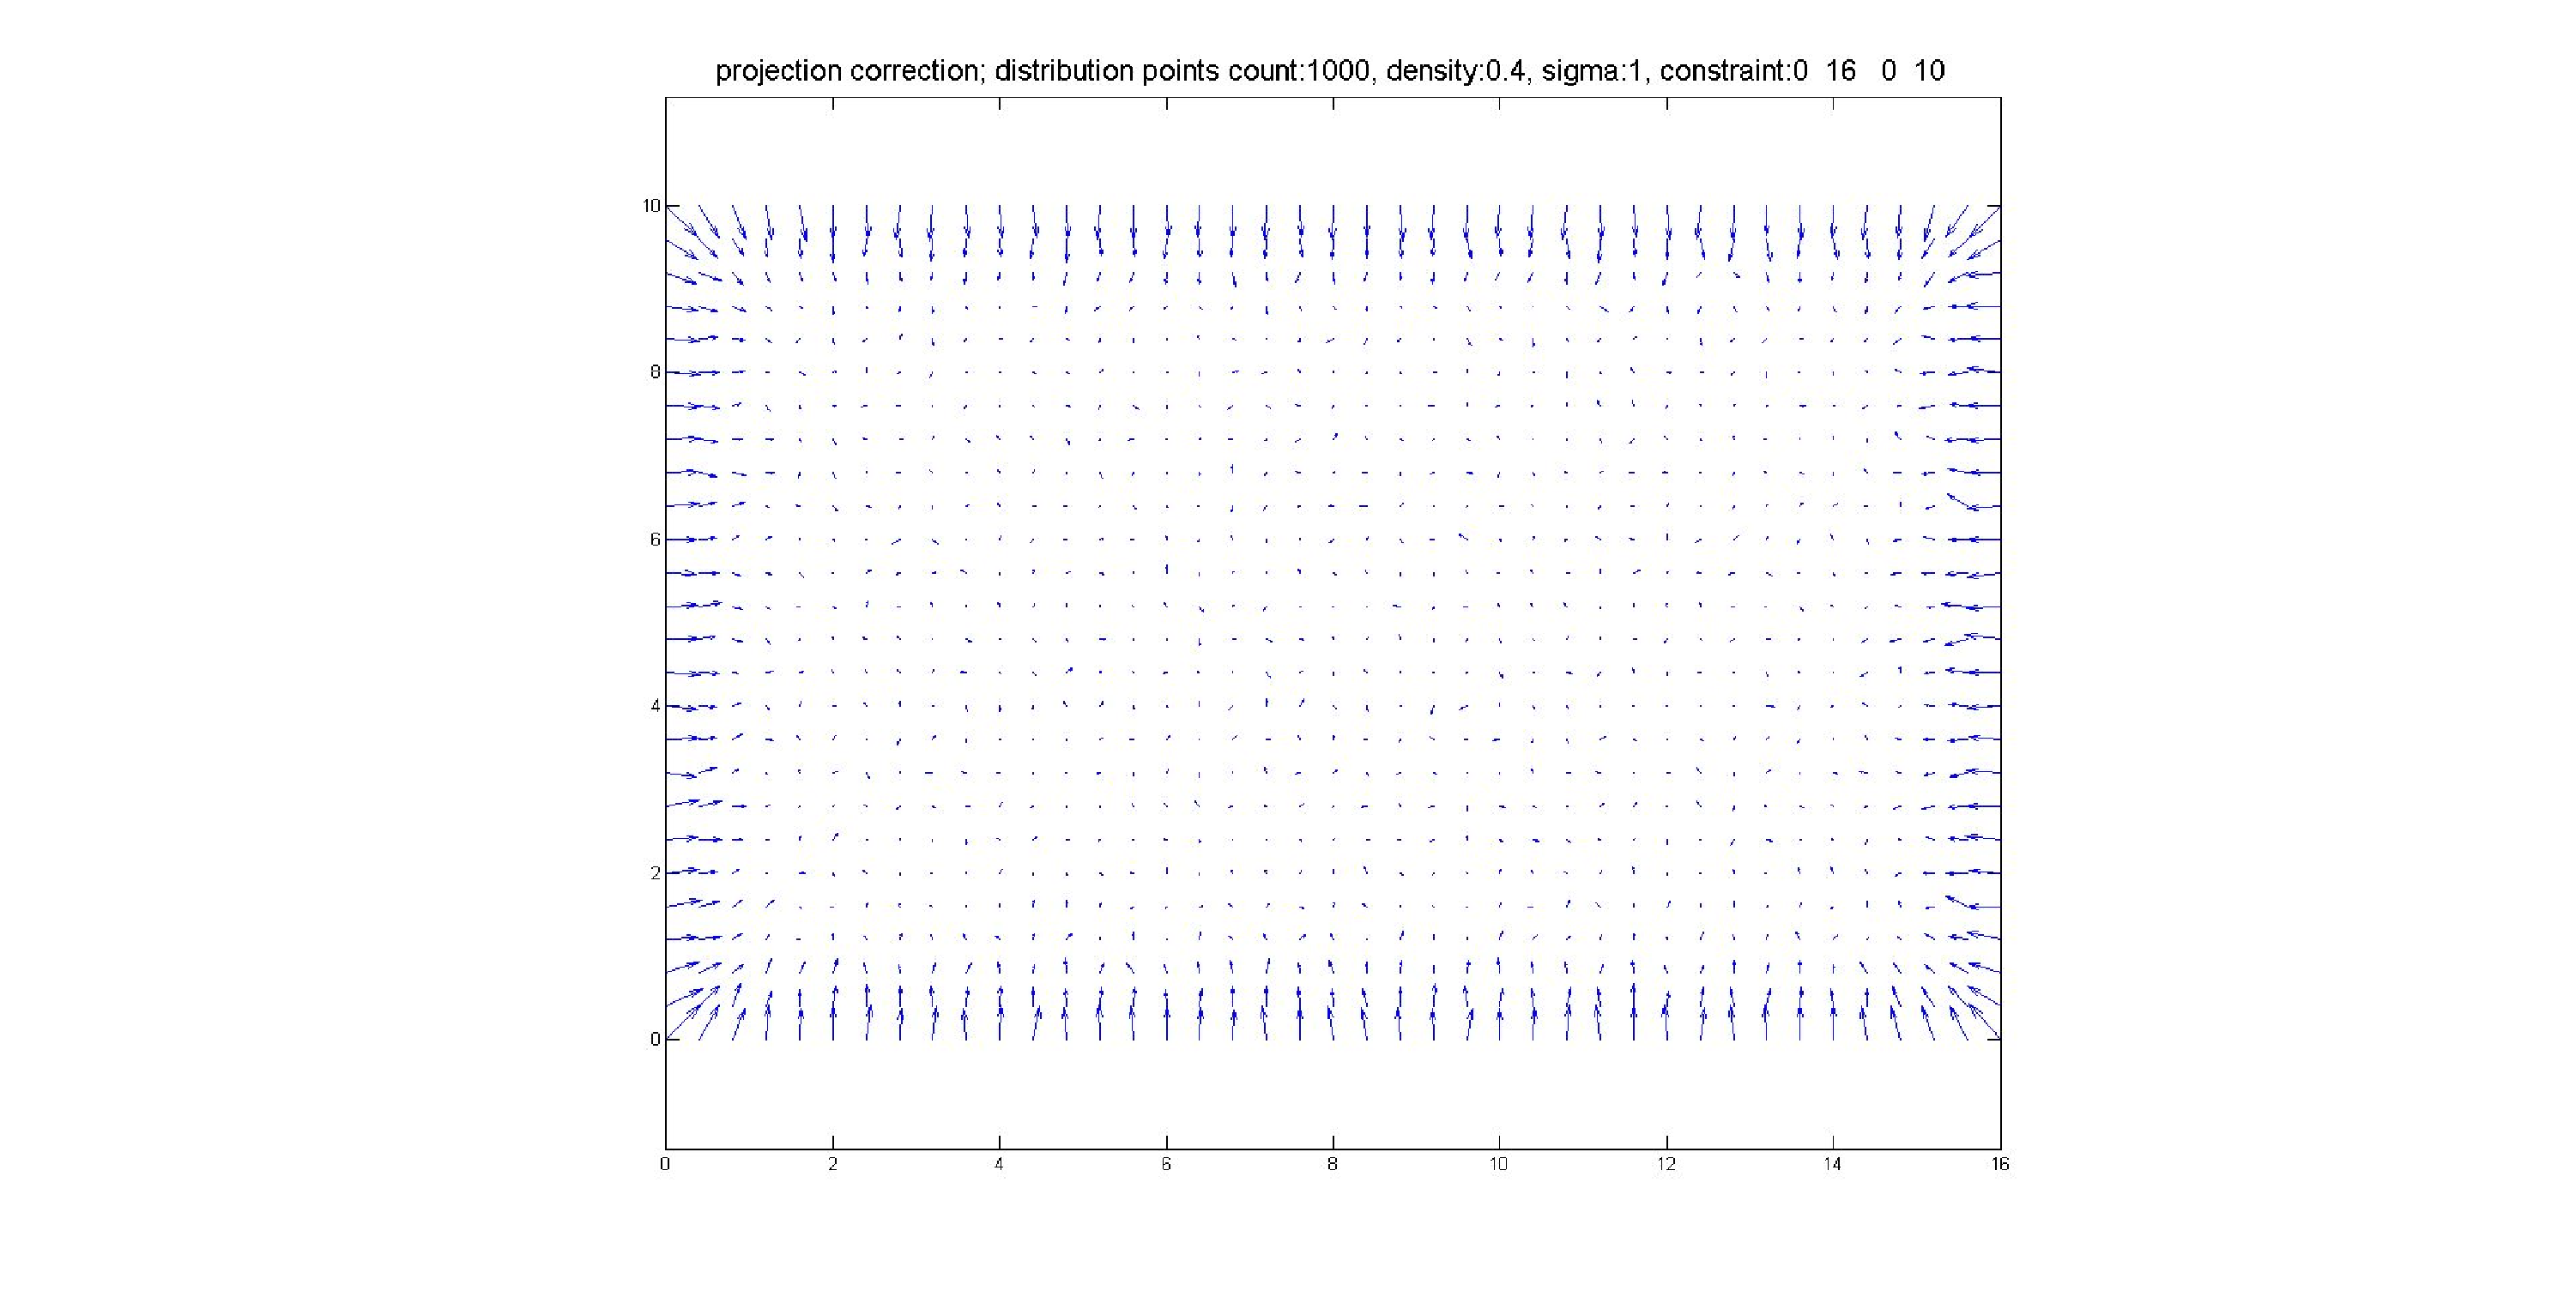
\includegraphics[width=\textwidth]{projection2dprzesuniecie}
\caption{Wykres wektorów przesunięć wartości oczekiwanych dla naprawy poprzez rzutowanie}
\end{figure}

\begin{figure}[H]
\centering
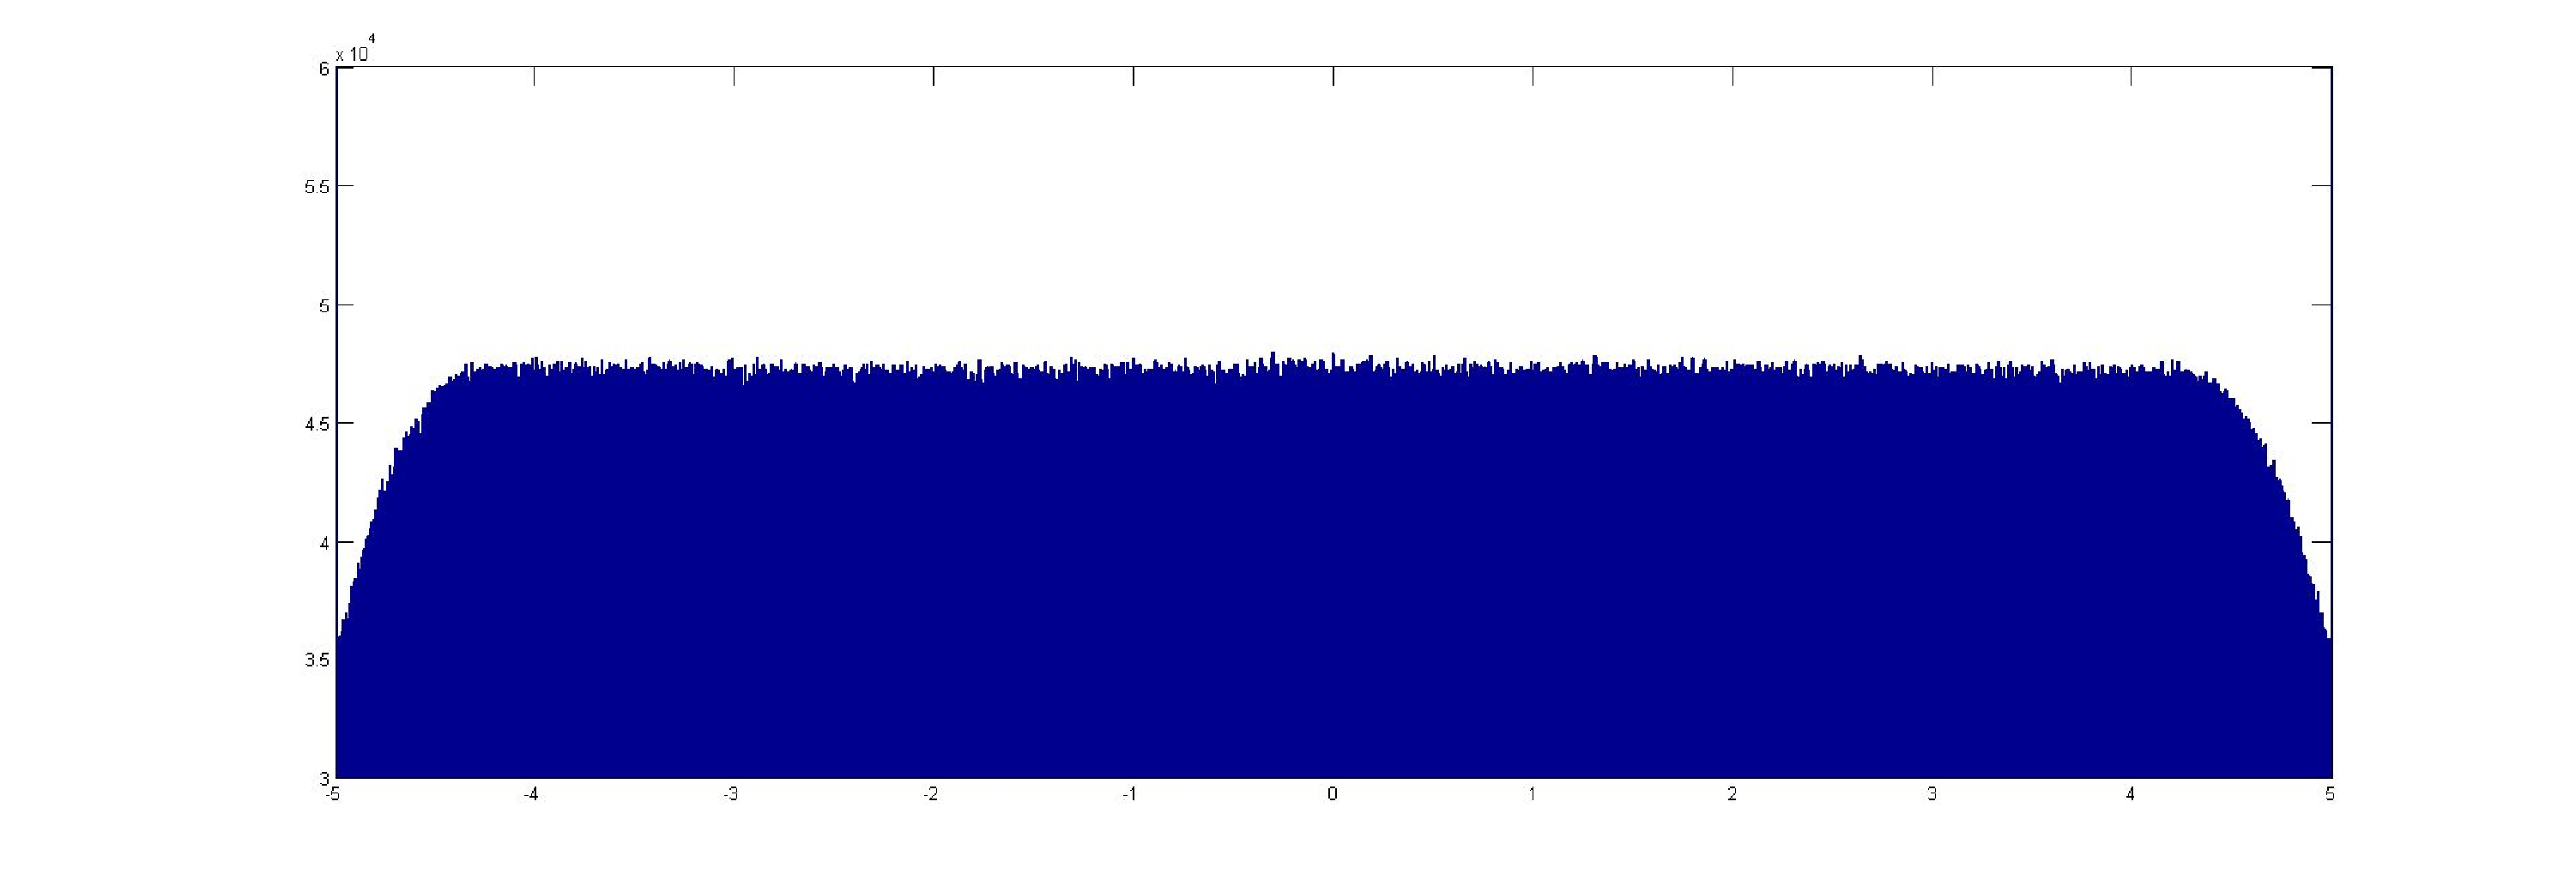
\includegraphics[width=\textwidth]{p_n_50M_1__5_5}
\caption{Histogram wystąpień punktów; naprawa poprzez rzutowanie; 1 wymiar; generowanie z rozkładem normalnym}
\label{bladzenie:rzutowanie1dn}
\end{figure}

\begin{figure}[H]
\centering
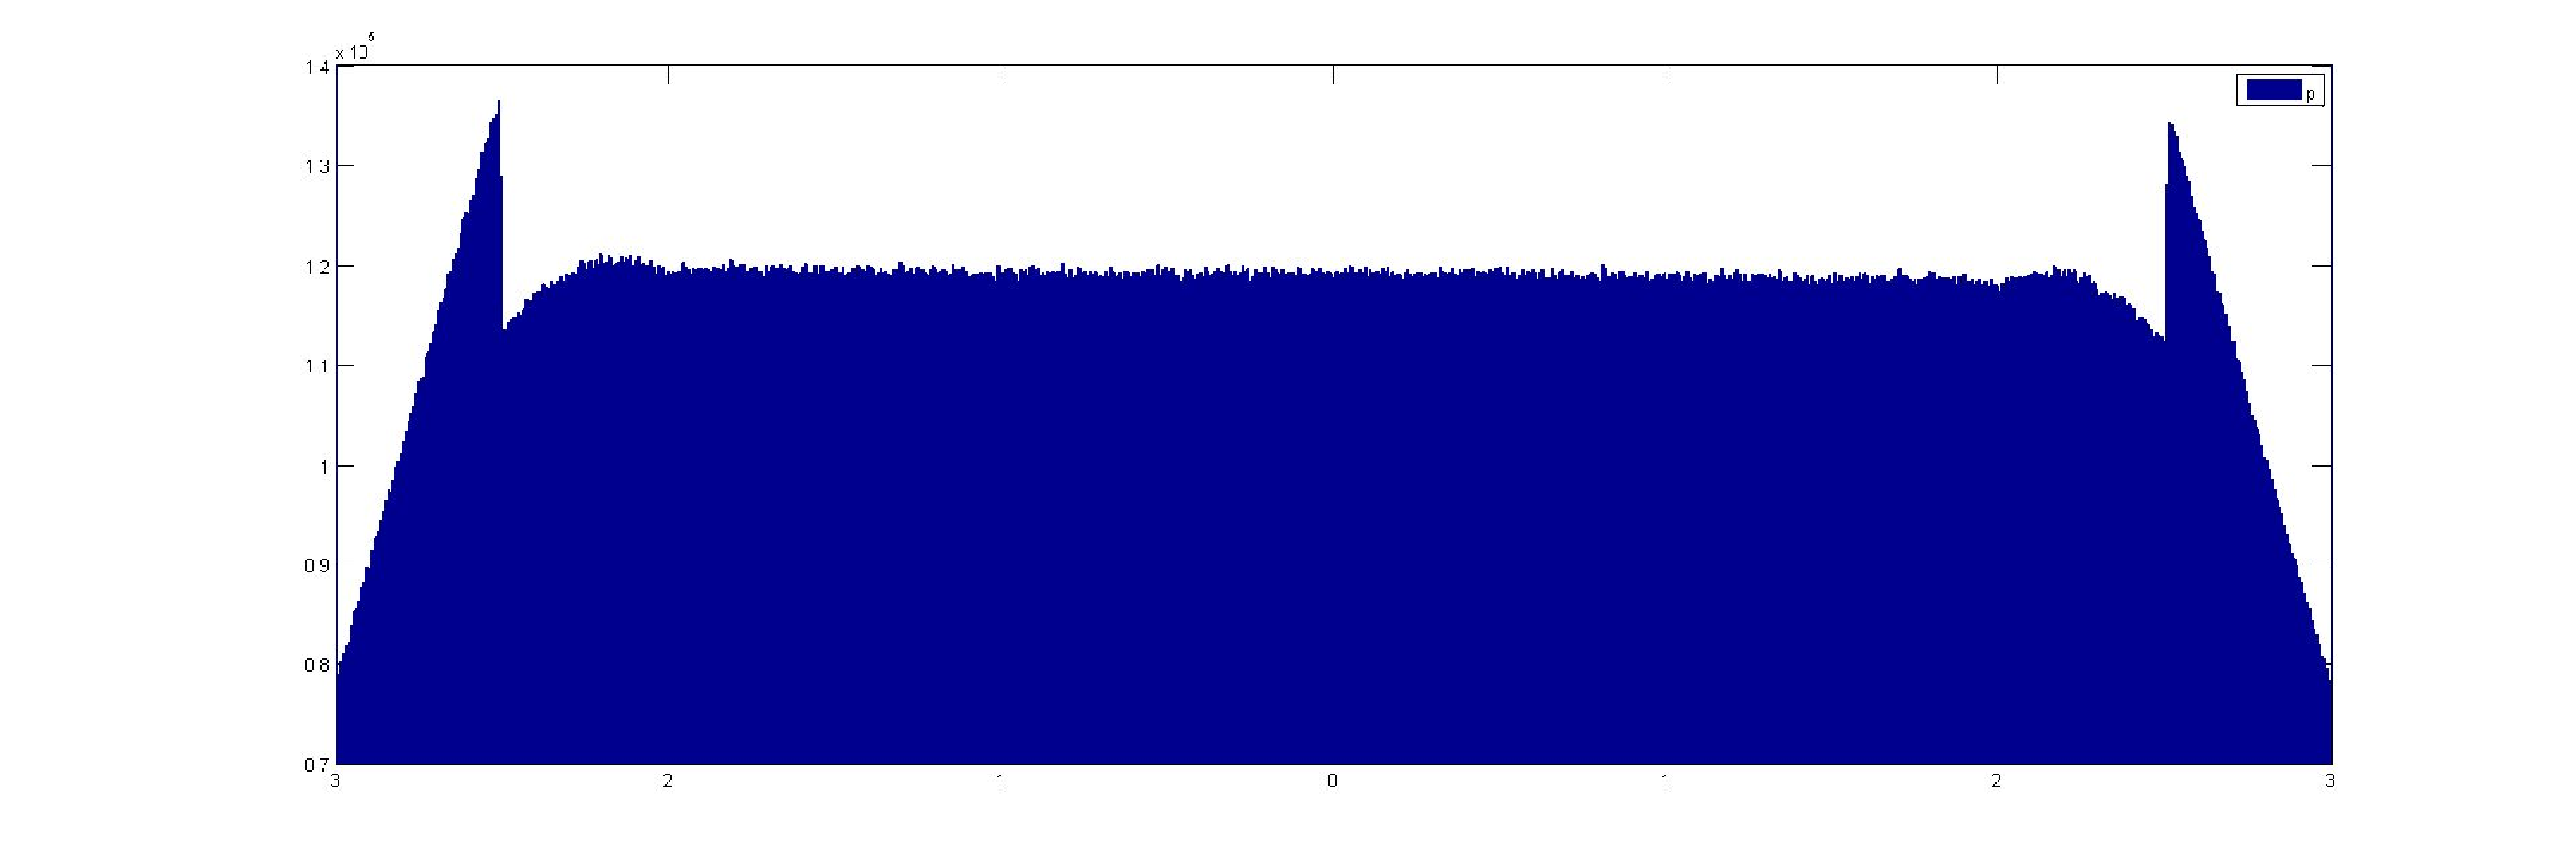
\includegraphics[width=\textwidth]{p_j_100M_1__3_3}
\caption{Histogram wystąpień punktów; naprawa poprzez rzutowanie; 1 wymiar; generowanie z rozkładem jednostajnym}
\label{bladzenie:rzutowanie1dj}
\end{figure}

\begin{figure}[H]
\centering
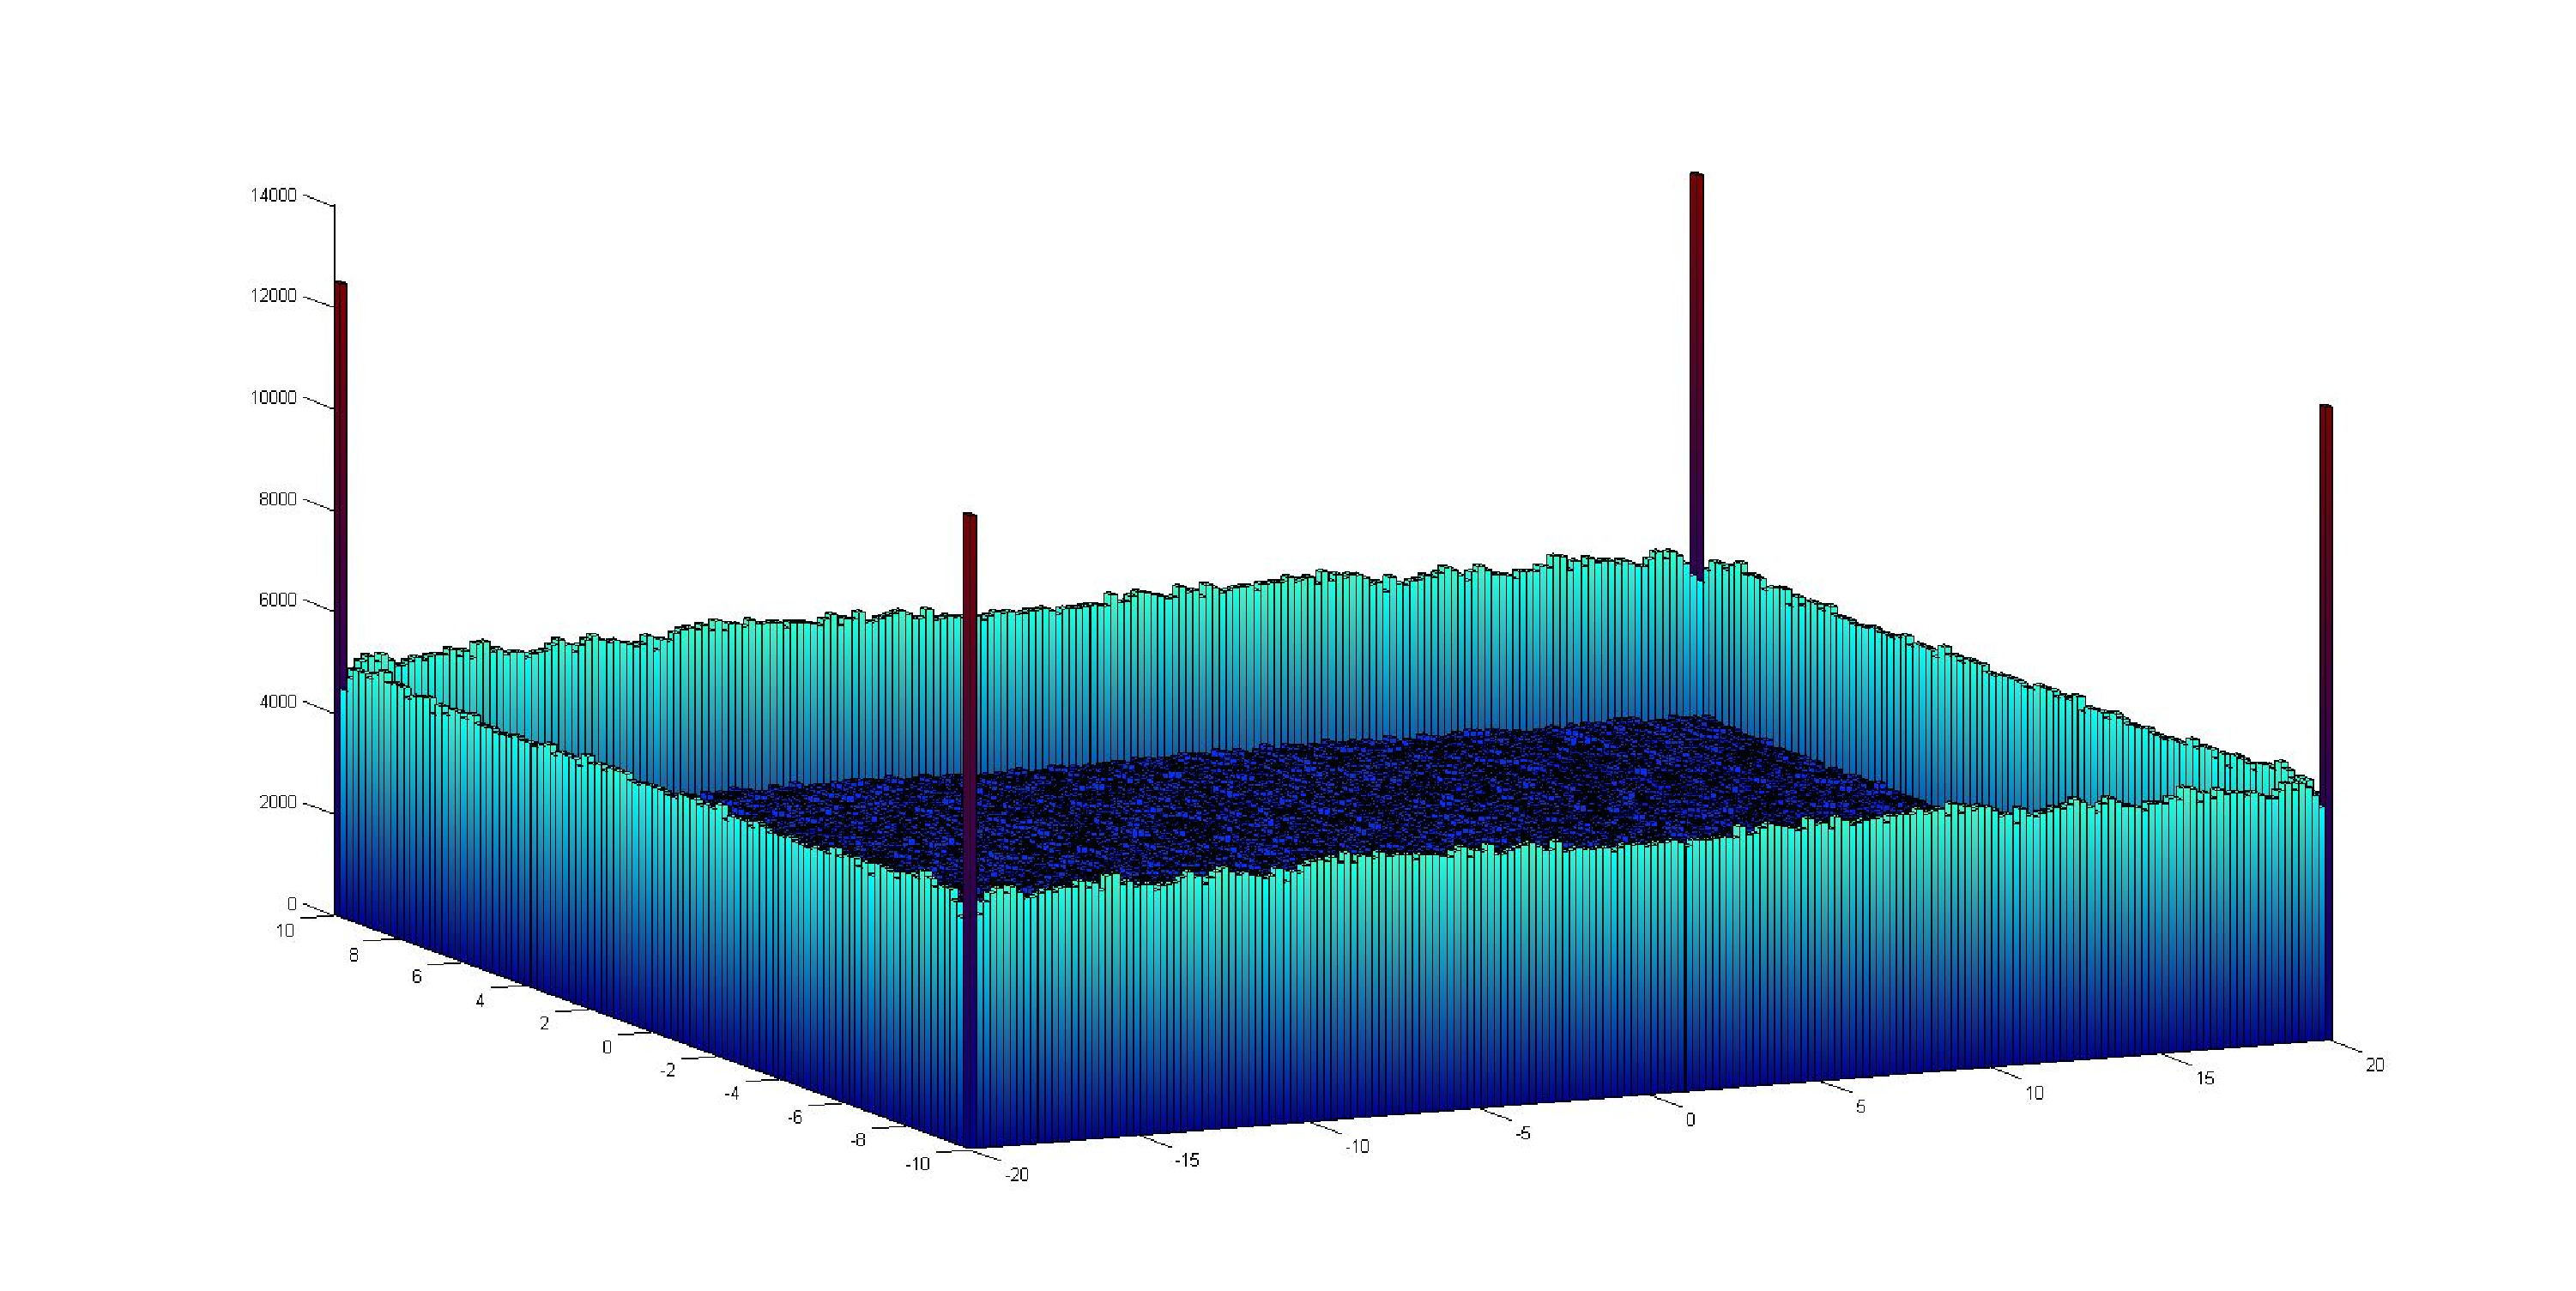
\includegraphics[width=\textwidth]{p_n_10M_2__20_20__10_10_4_2}
\caption{Histogram wystąpień punktów; naprawa poprzez rzutowanie; 2 wymiary; generowanie z rozkładem normalnym}
\label{bladzenie:rzutowanie2d}
\end{figure}

\subsubsection*{Reinicjacja}
\hspace{3,4ex}Wykres wartości oczekiwanych jest mało czytelny, ponieważ wartości przesunięć są duże. Ma w tym udział reinicjacja, która przesuwa część punktów na środek przestrzeni przeszukiwań.

Histogramy nie ukazują nic nadzwyczajnego, ponieważ łatwo zauważyć pik związany z reinicjacją oraz wartości histogramu malejące wraz ze zbliżaniem się do ograniczeń. Warto jednak zwrócić uwagę na dwa fakty.

Pierwsze spostrzeżenie, to kształt histogramu. Zarówno dla rozkładu jednostajnego, jak i normalnego w jednym wymiarze jest on stożkowy. Łuk można zauważyć tylko blisko punktu środkowego, w pozostałej części spadek jest liniowy. Brakuje charakterystycznego, gaussowskiego przegięcia. Sytuacja jest ciekawsza, gdy występuje więcej wymiarów. Widać wówczas przegięcie (Rysunek \ref{bladzenie:reinicjacja2ds}). Dokładniejsze badania pokazały, że przegięcie nie występuje tylko na jednym wymiarze - tym, który jest relatywnie najkrótszy. Celowo jest użyte słowo relatywnie, ponieważ z~perspektywy błądzenia przypadkowego i~rozkładu normalnego trzeba brać pod uwagę parametr $\sigma$ - odchylenie standardowe zmiennej losowej. Wymiary o małym $\sigma$ będą relatywnie dłuższe od tych z dużym $\sigma$, ponieważ błądzenie będzie wykonywało mniejsze kroki.

Na rysunku \ref{bladzenie:reinicjacja1dj} można dostrzec też dwa uskoki, które związane są z pikiem w punkcie~$0$ oraz charakterystyką rozkładu jednostajnego.

\begin{figure}[H]
\centering
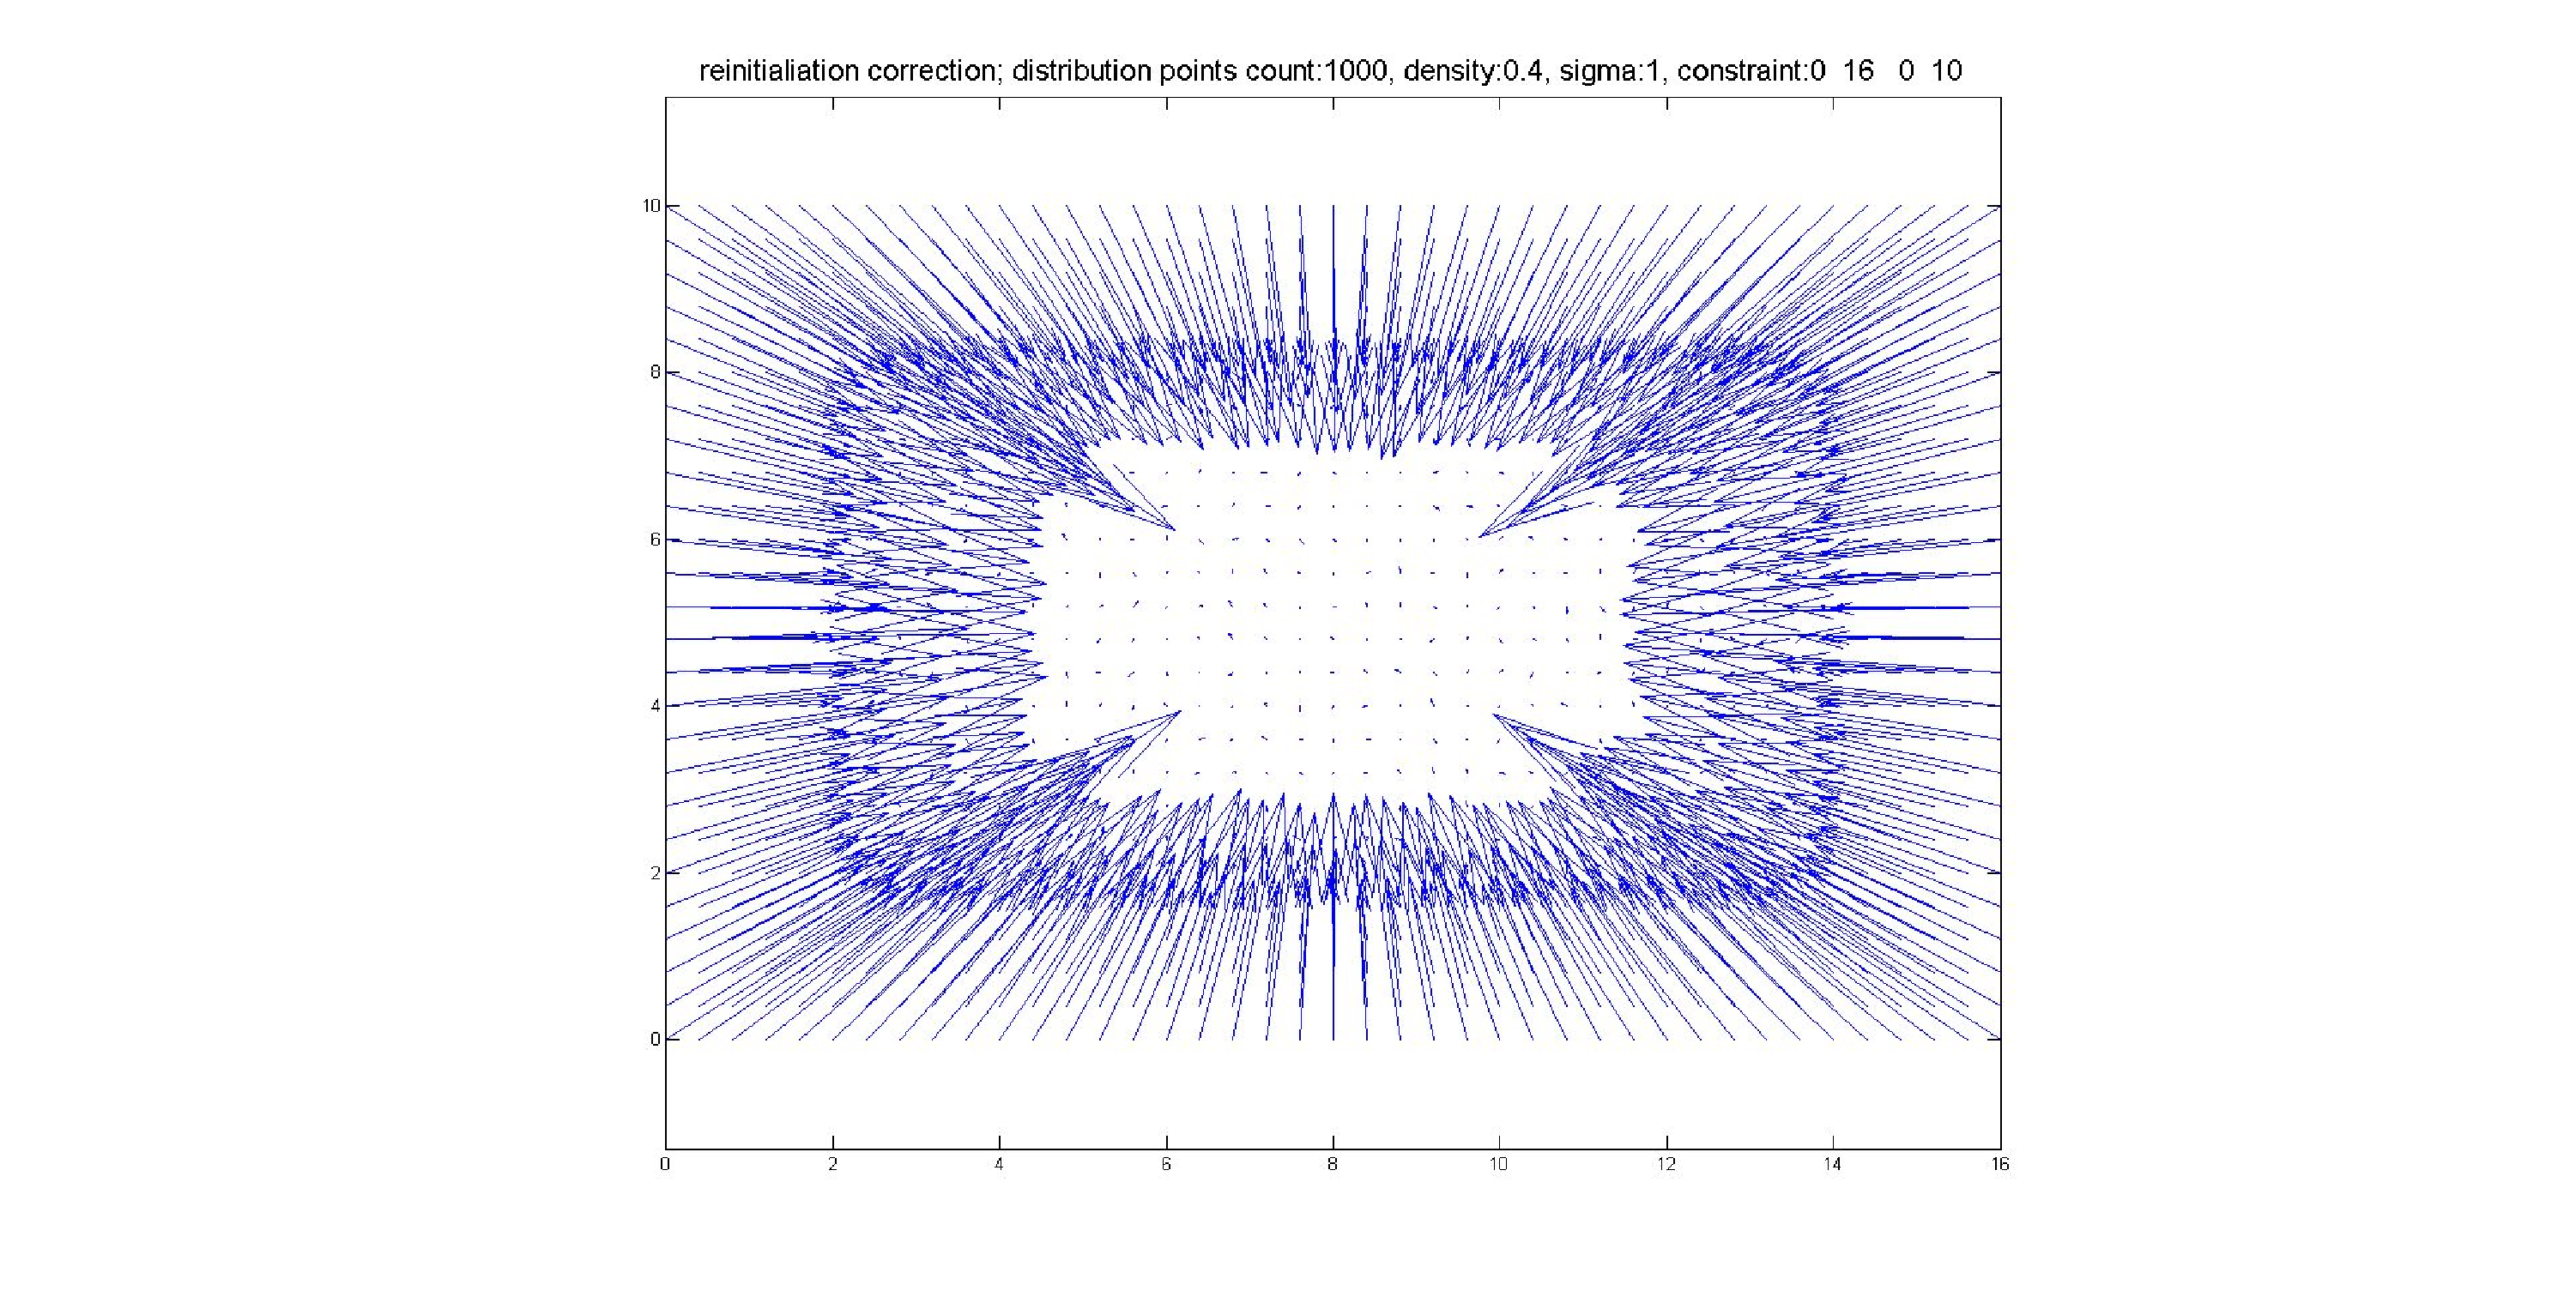
\includegraphics[width=\textwidth]{reinitialization2dprzesuniecie}
\caption{Wykres wektorów przesunięć wartości oczekiwanych dla naprawy poprzez reinicjację}
\end{figure}

\begin{figure}[H]
\centering
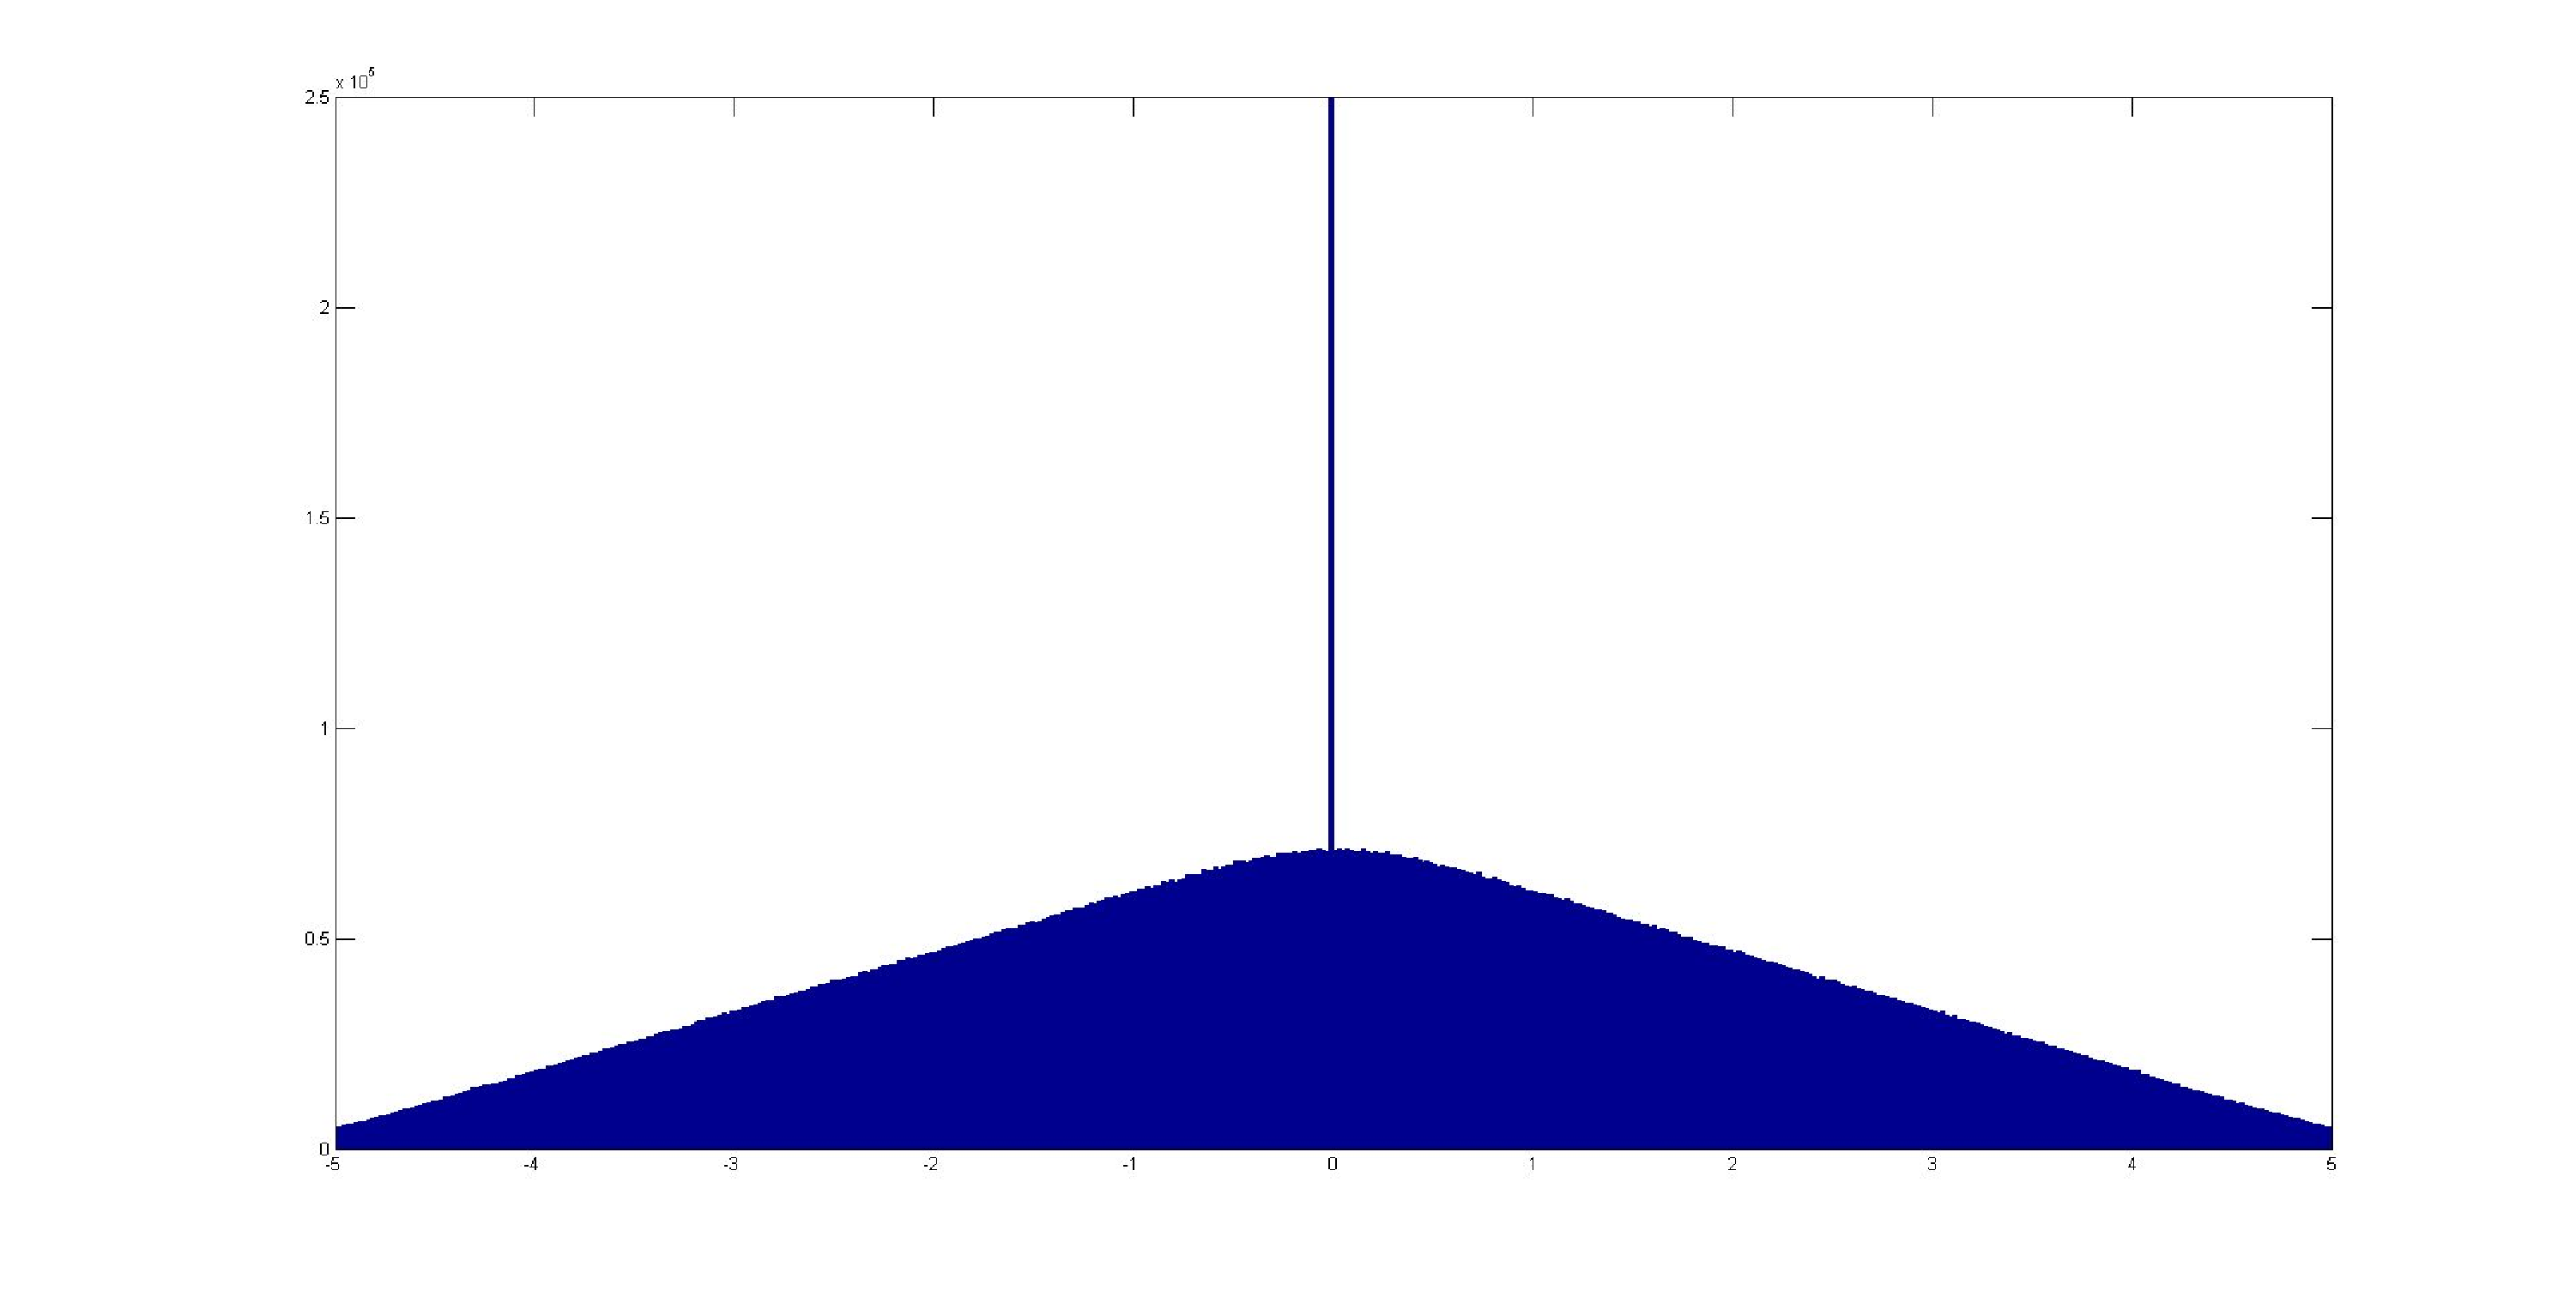
\includegraphics[width=\textwidth]{ri_n_20M_1__5_5}
\caption{Histogram wystąpień punktów; naprawa poprzez reinicjację; 1 wymiar; generowanie z rozkładem normalnym}
\end{figure}

\begin{figure}[H]
\centering
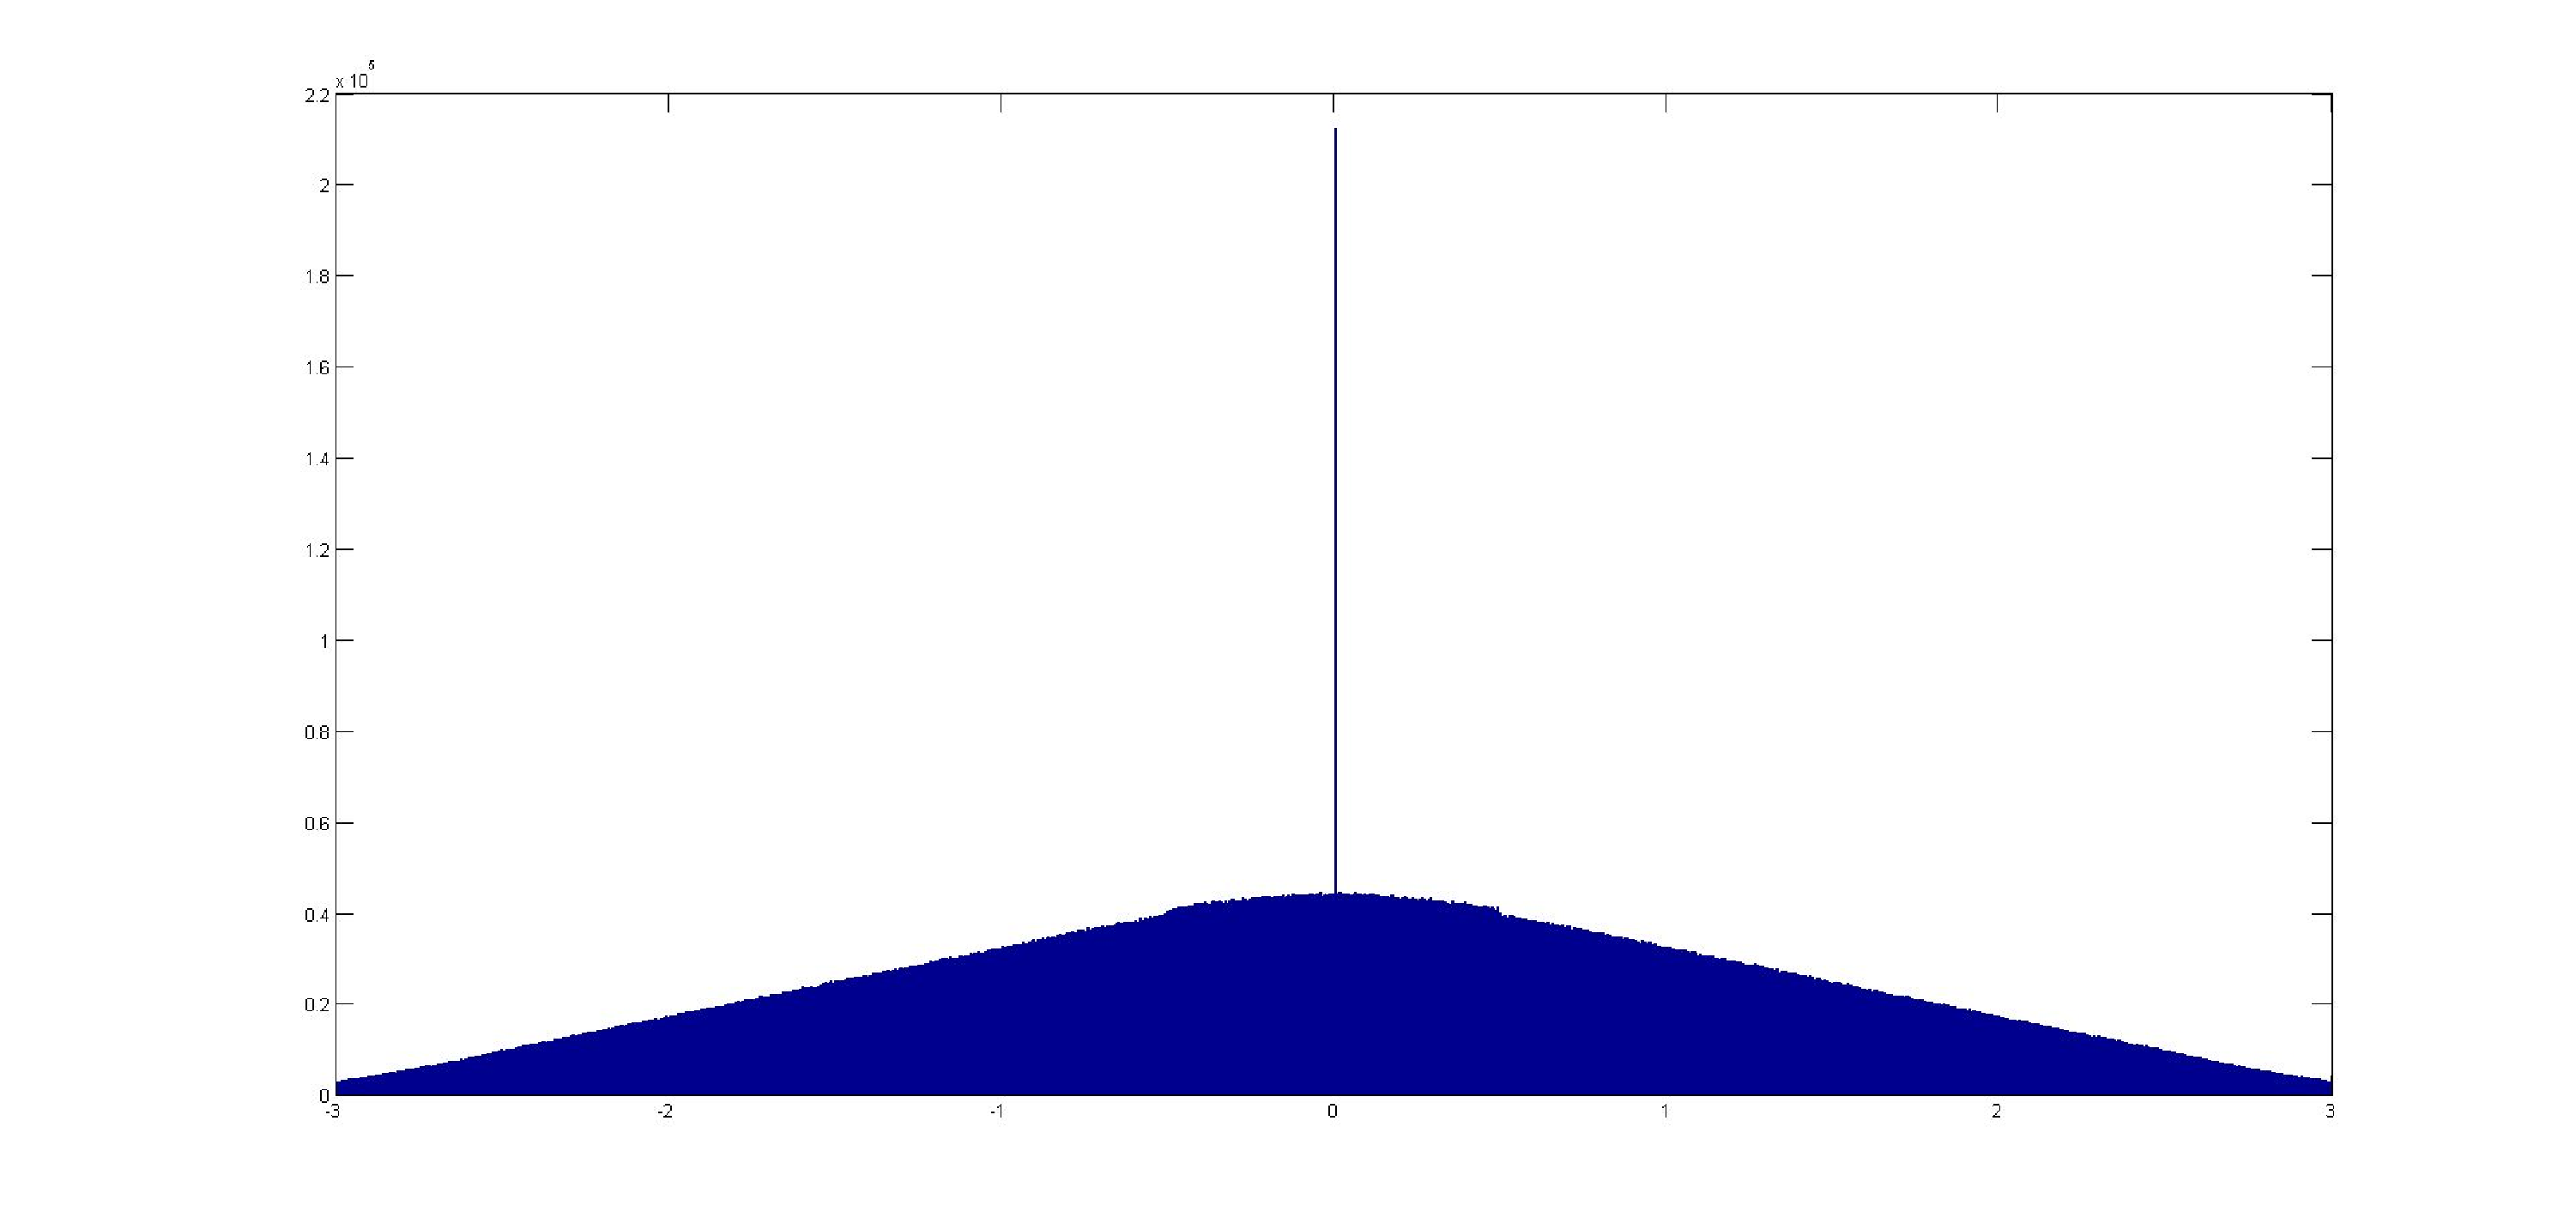
\includegraphics[width=\textwidth]{ri_j_20M_1__3_3}
\caption{Histogram wystąpień punktów; naprawa poprzez reinicjację; 1 wymiar; generowanie z rozkładem jednostajnym}
\label{bladzenie:reinicjacja1dj}
\end{figure}

\begin{figure}[H]
\centering
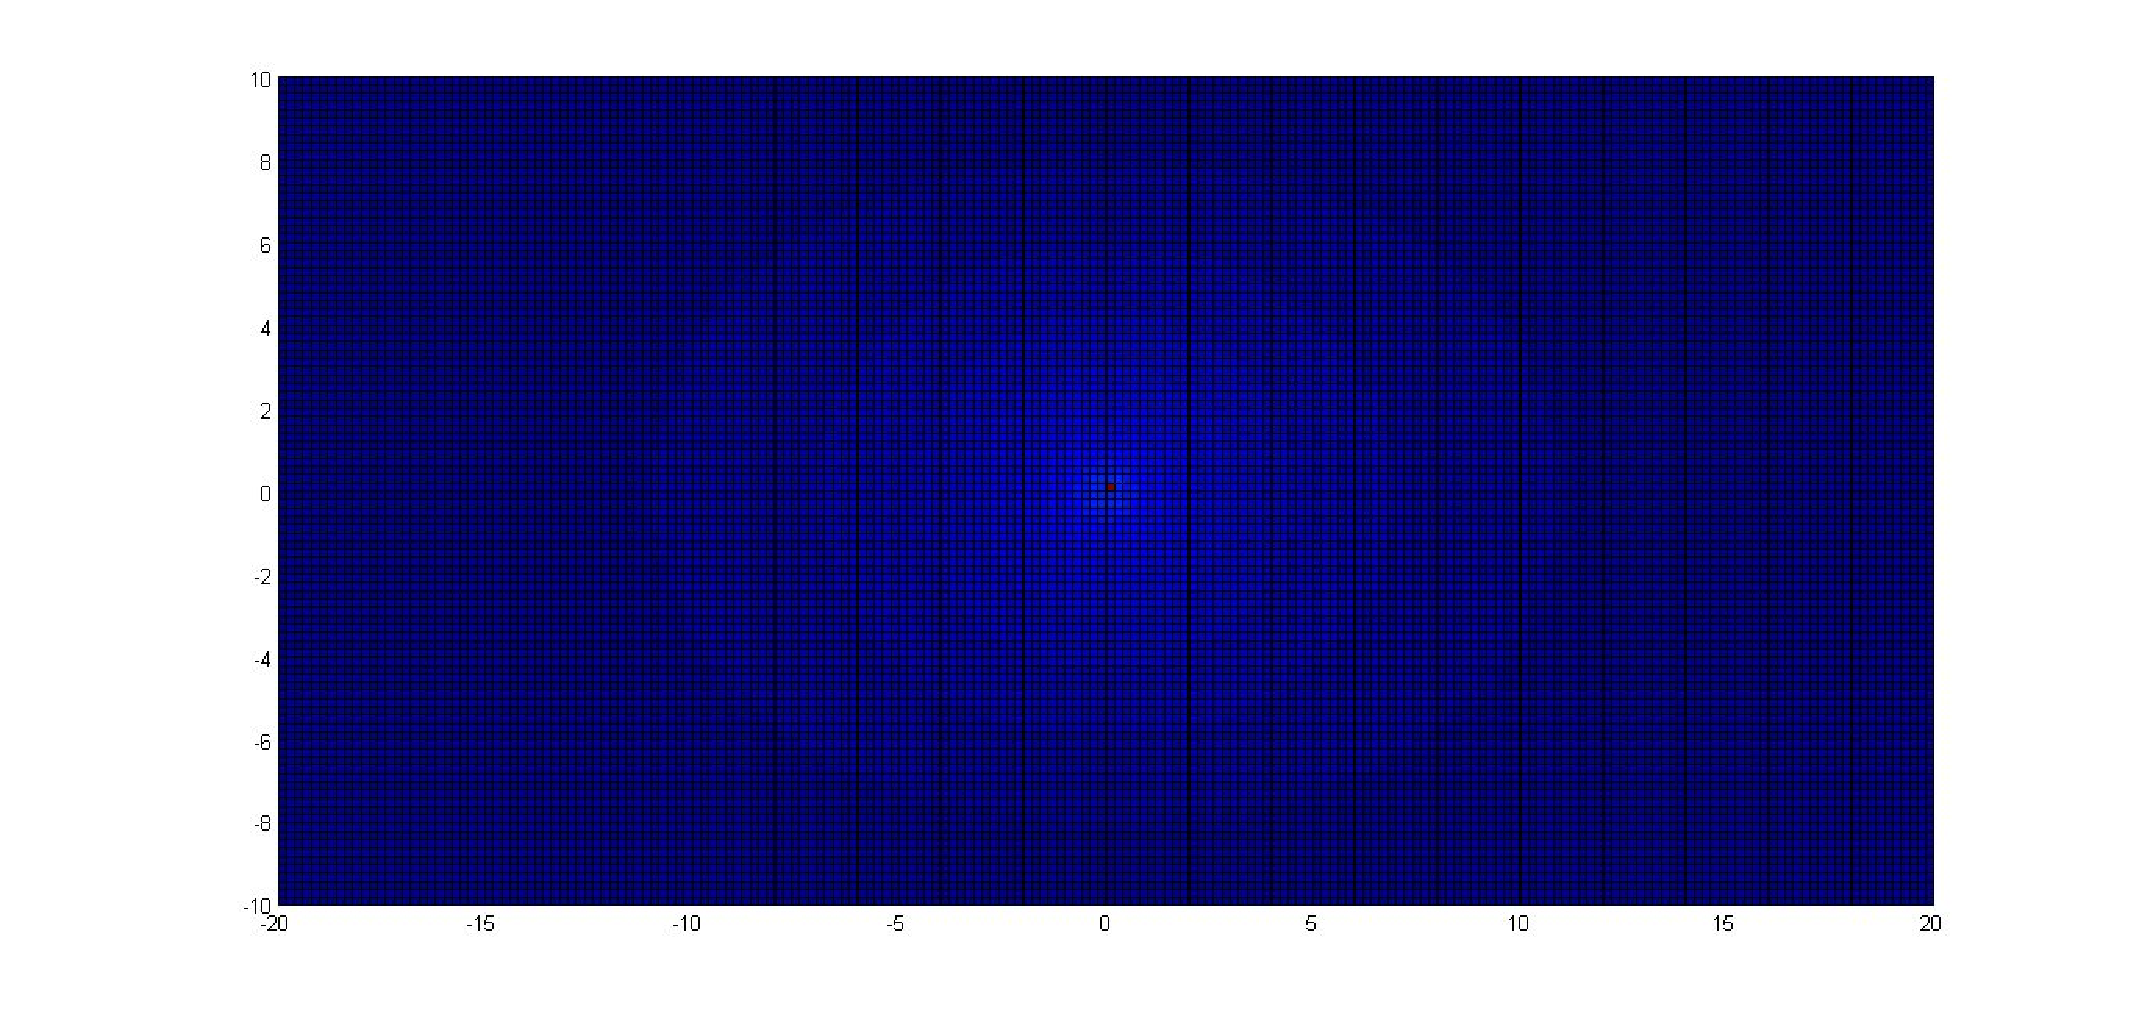
\includegraphics[width=\textwidth]{ri_n_10M_2__20_20__10_10_4}
\caption{Histogram wystąpień punktów; naprawa poprzez reinicjację; 2 wymiary; generowanie z rozkładem normalnym}
\end{figure}

\begin{figure}[H]
\centering
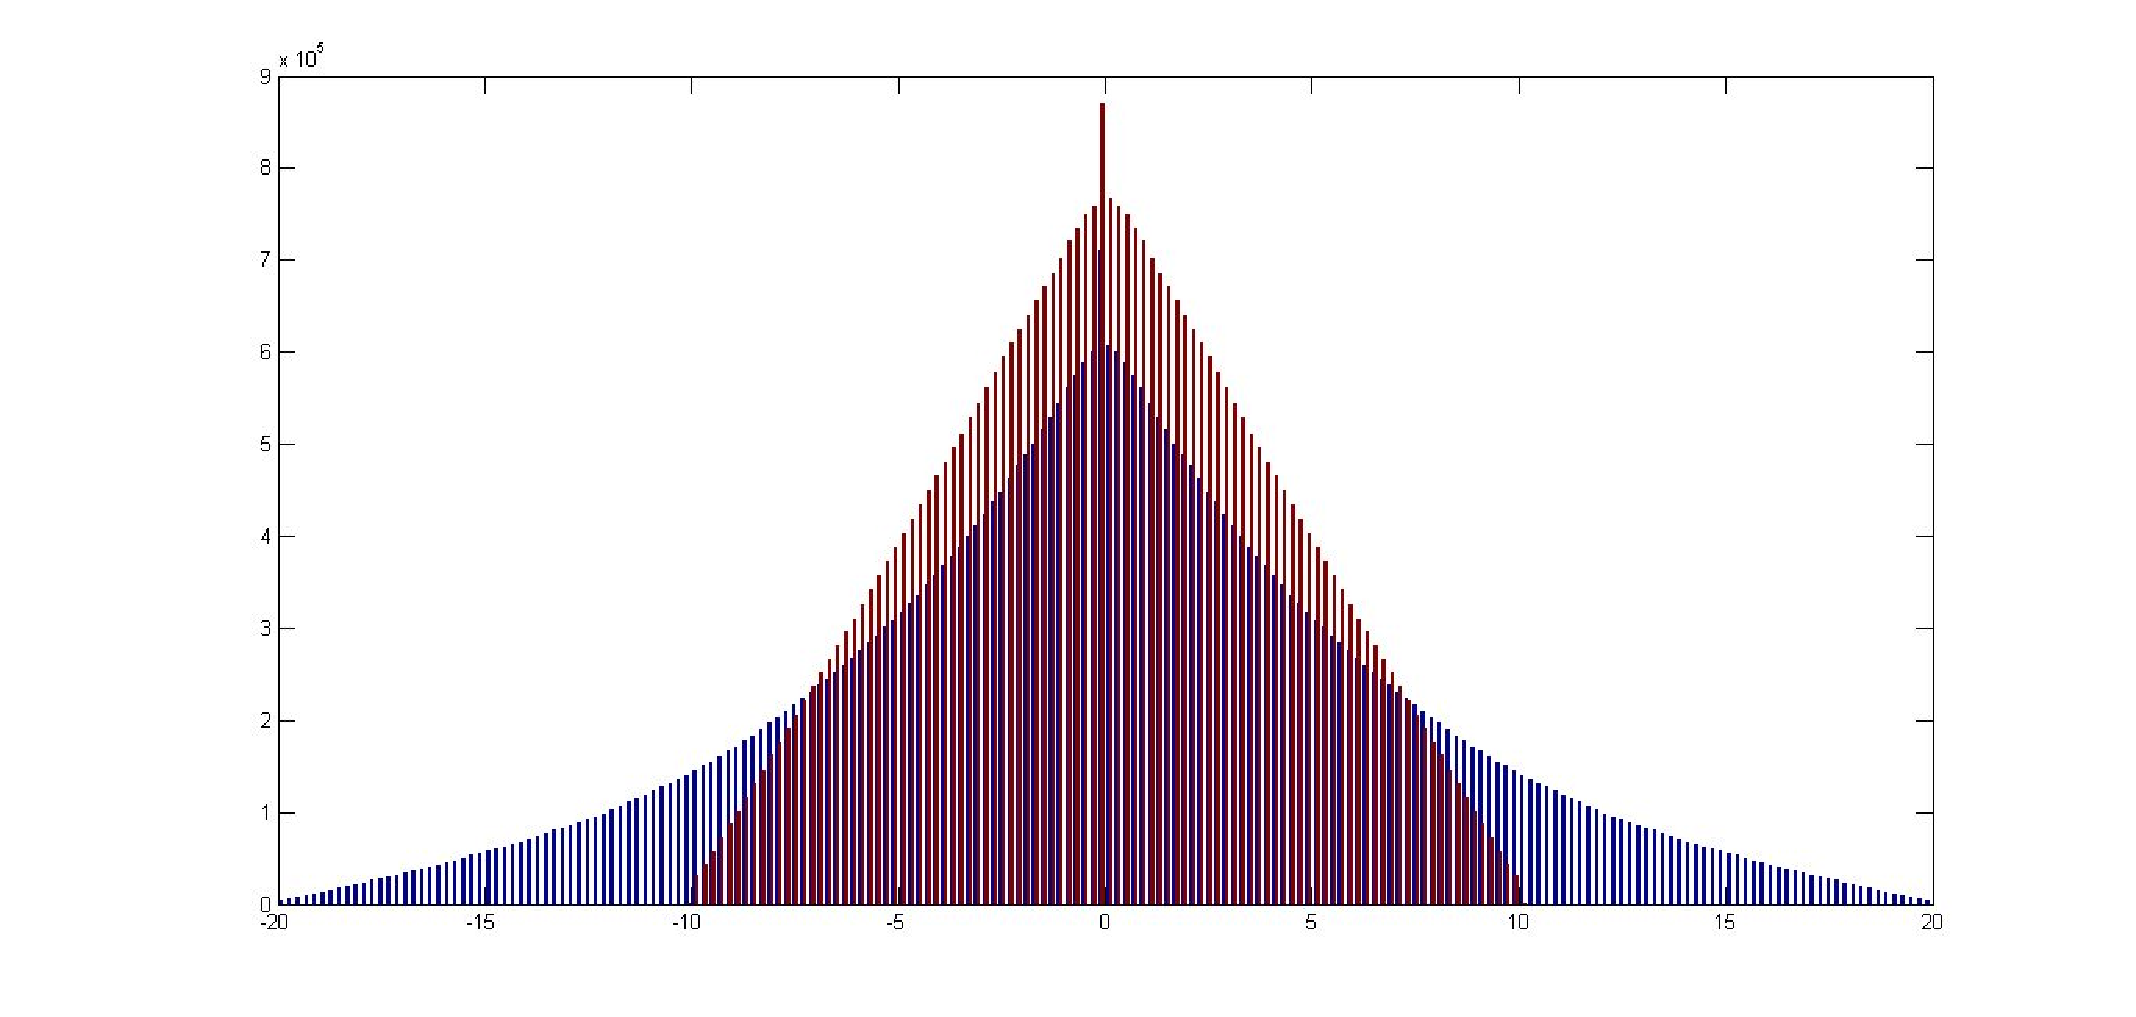
\includegraphics[width=\textwidth]{ri_n_10M_2__20_20__10_10_4_1D}
\caption{Histogram wystąpień punktów; naprawa poprzez reinicjację; 2 wymiary; generowanie z rozkładem normalnym; oddzielne histogramy dla obu wymiarów}
\label{bladzenie:reinicjacja2ds}
\end{figure}

\subsubsection*{Powtórna generacja}
\hspace{3,4ex}Ten rozkład charakteryzuje się spadkiem wartości gęstości punktów wraz ze zbliżaniem się do ograniczenia. Punkty, które wypadłyby poza ograniczenia oraz ich potomkowie są przesuwane w kierunku środka przedziału.

\begin{figure}[H]
\centering
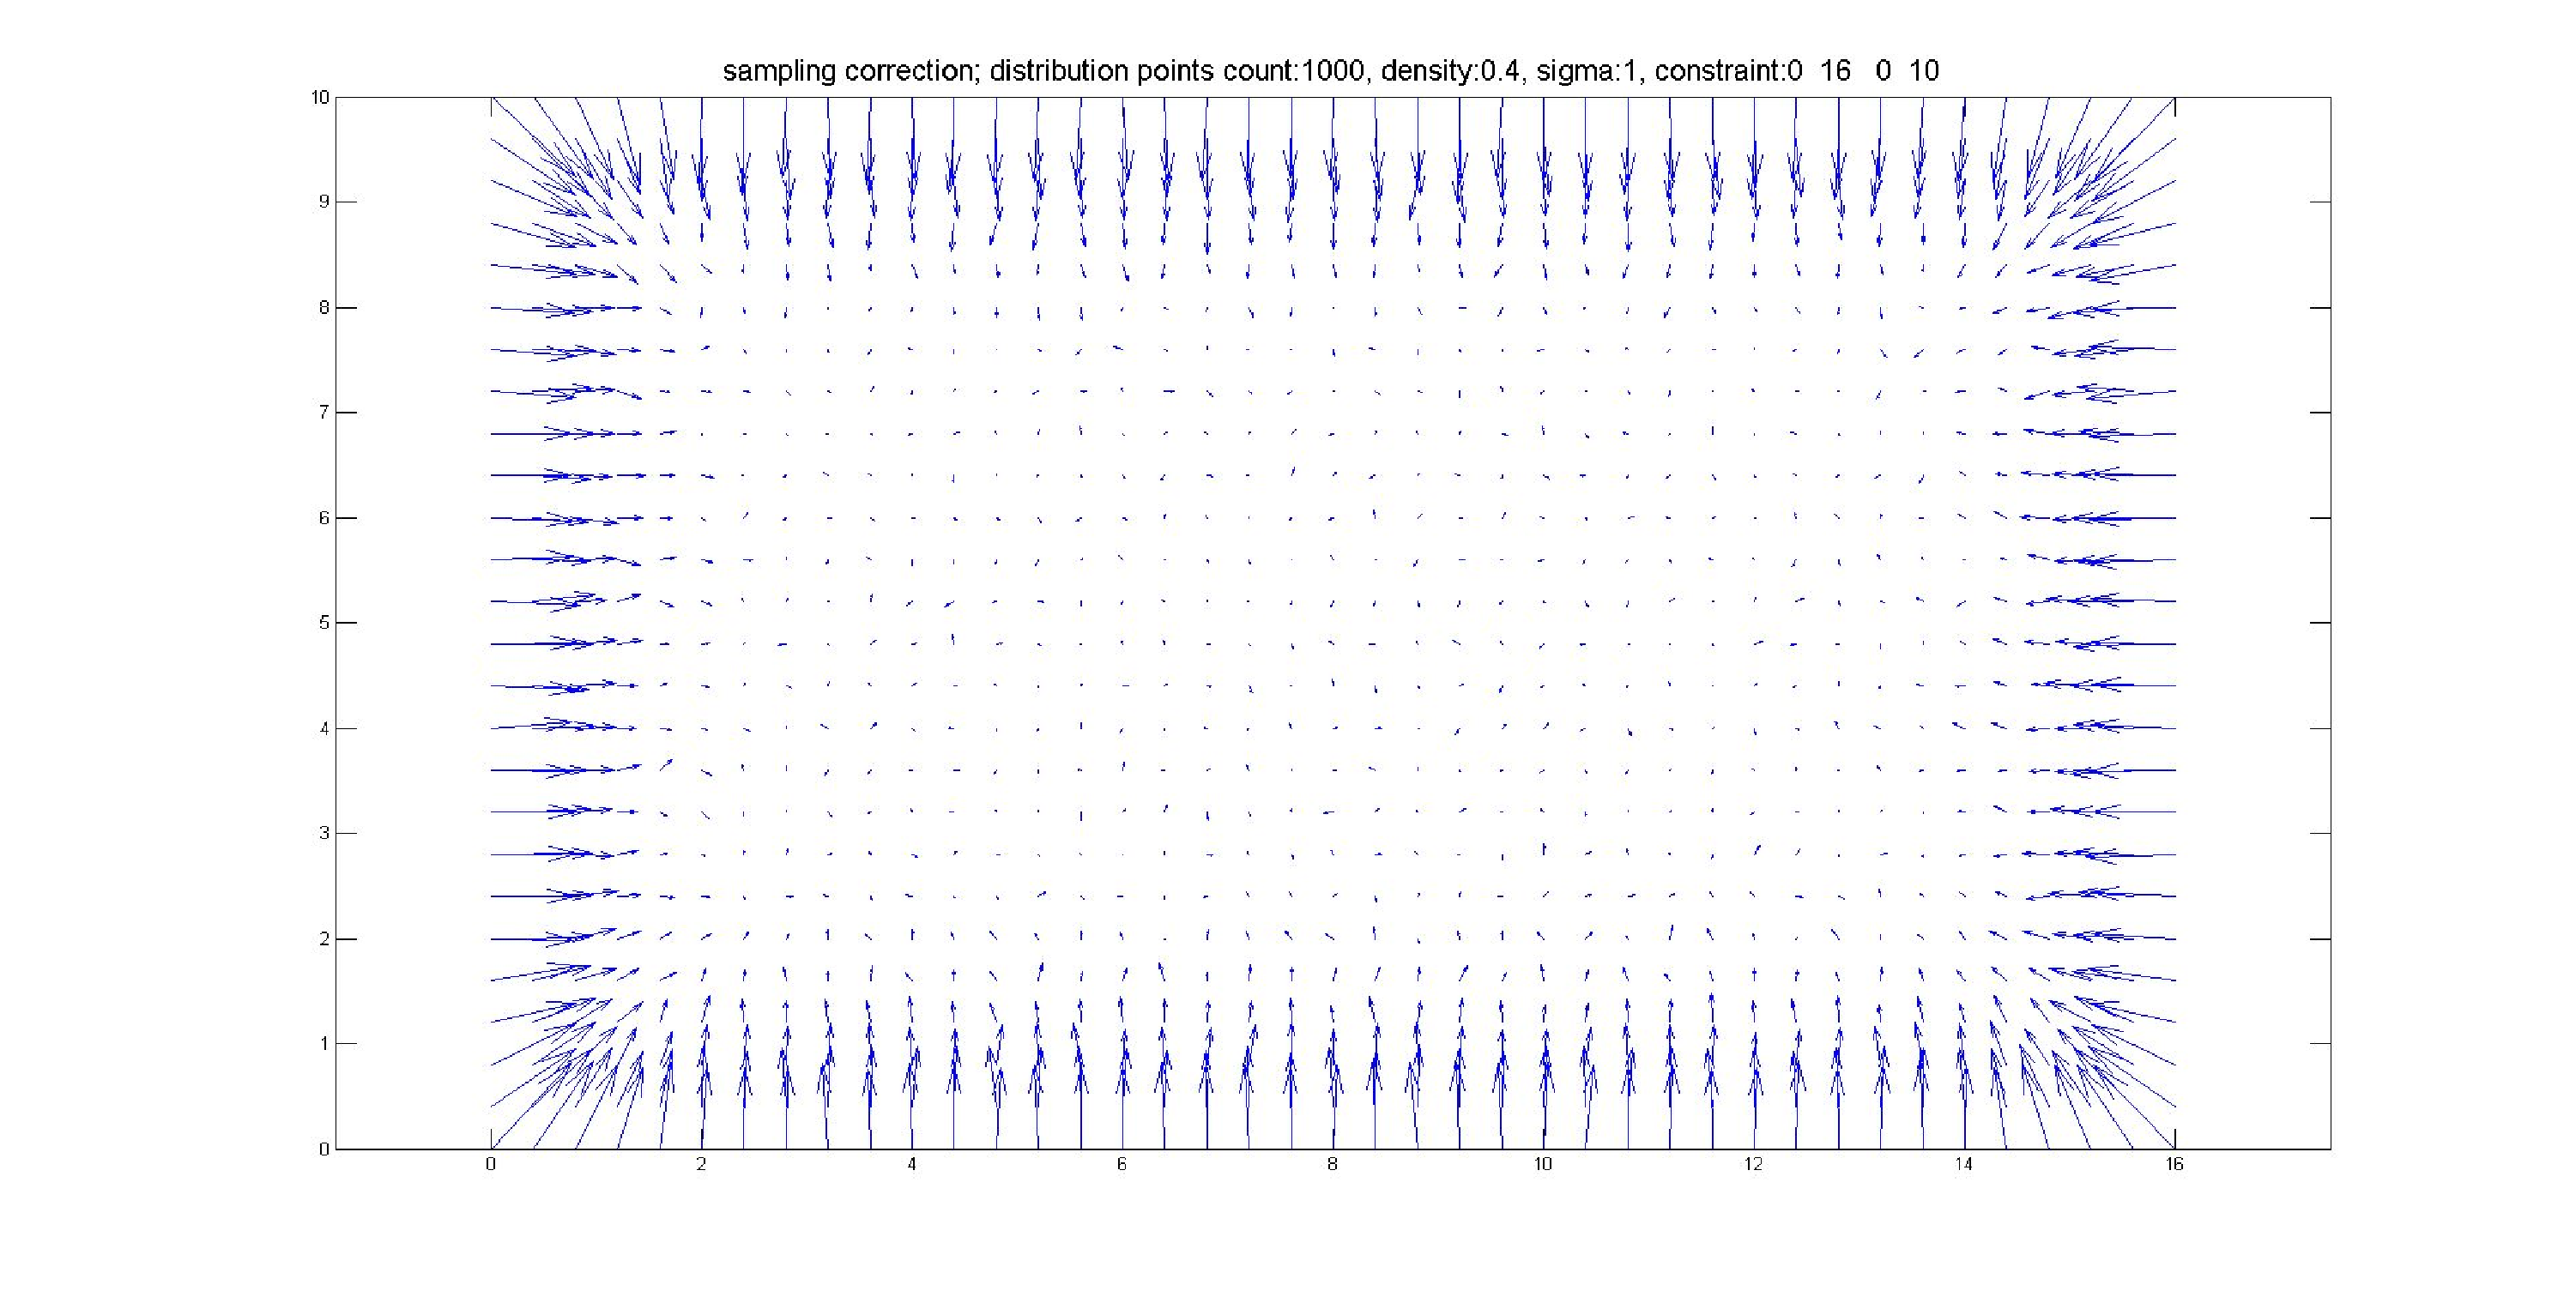
\includegraphics[width=\textwidth]{sampling2dprzesuniecie}
\caption{Wykres wektorów przesunięć wartości oczekiwanych dla metody naprawy poprzez powtórną generację}
\end{figure}

\begin{figure}[H]
\centering
\subfloat[Generowanie z rozkładem normalnym]{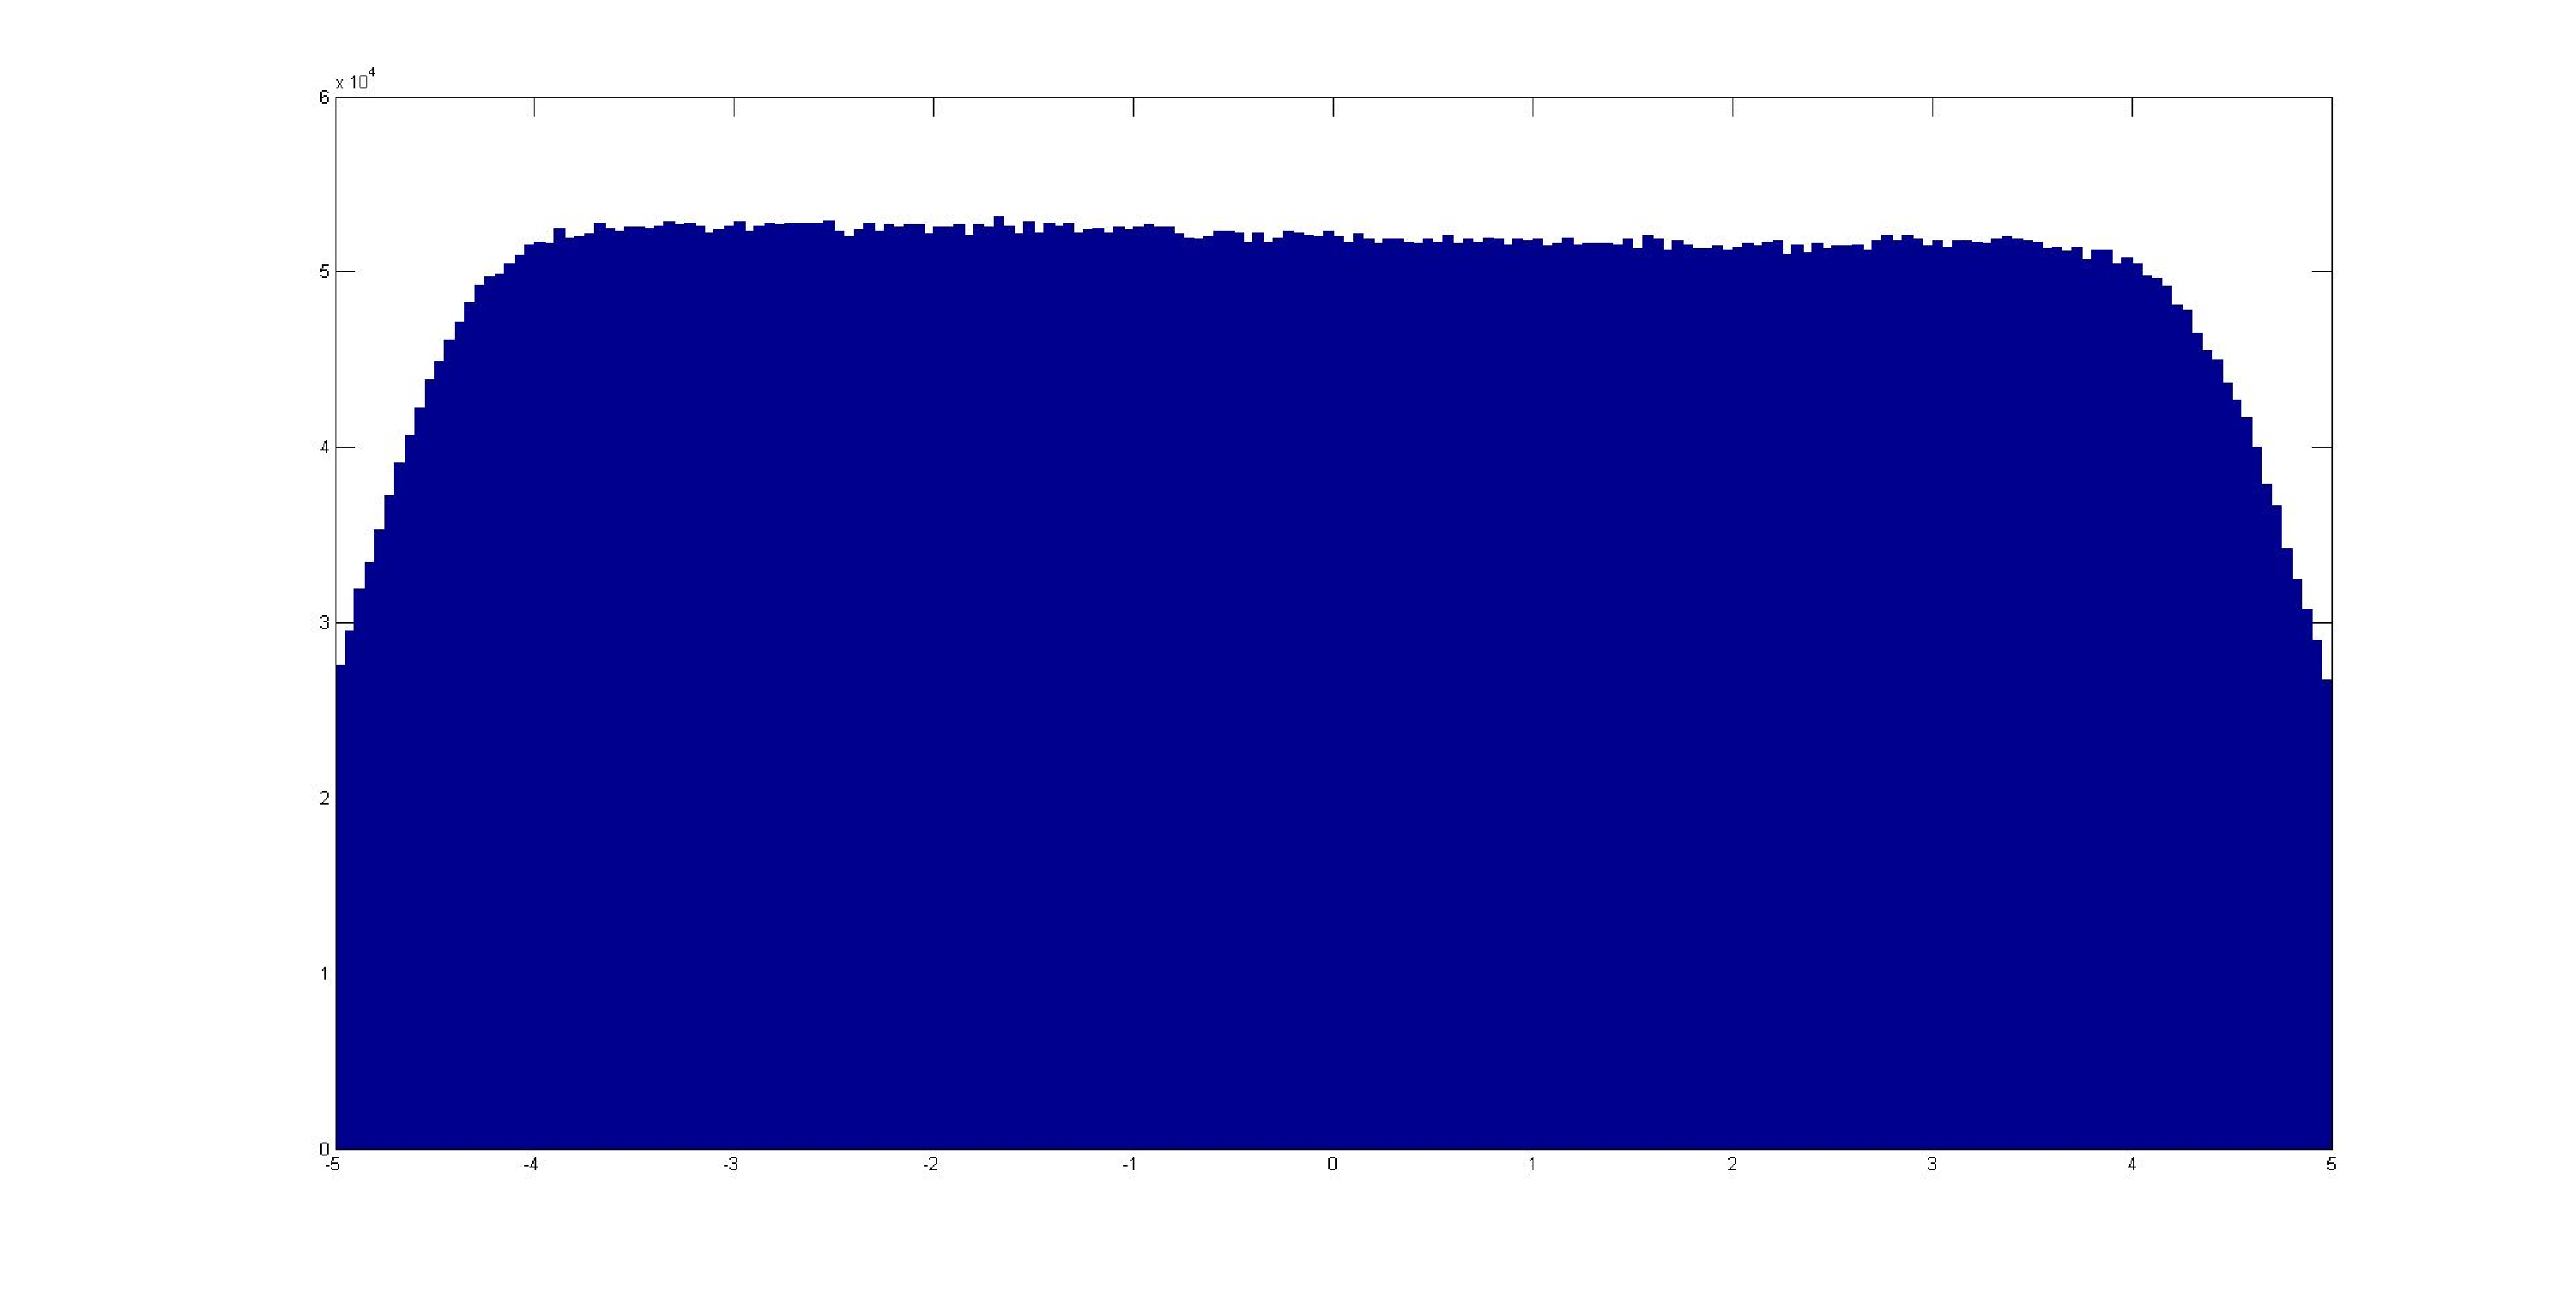
\includegraphics[width=0.45\textwidth]{s_n_10M_1__5_5}}
\quad
\subfloat[Generowanie z rozkładem jednostajnym]{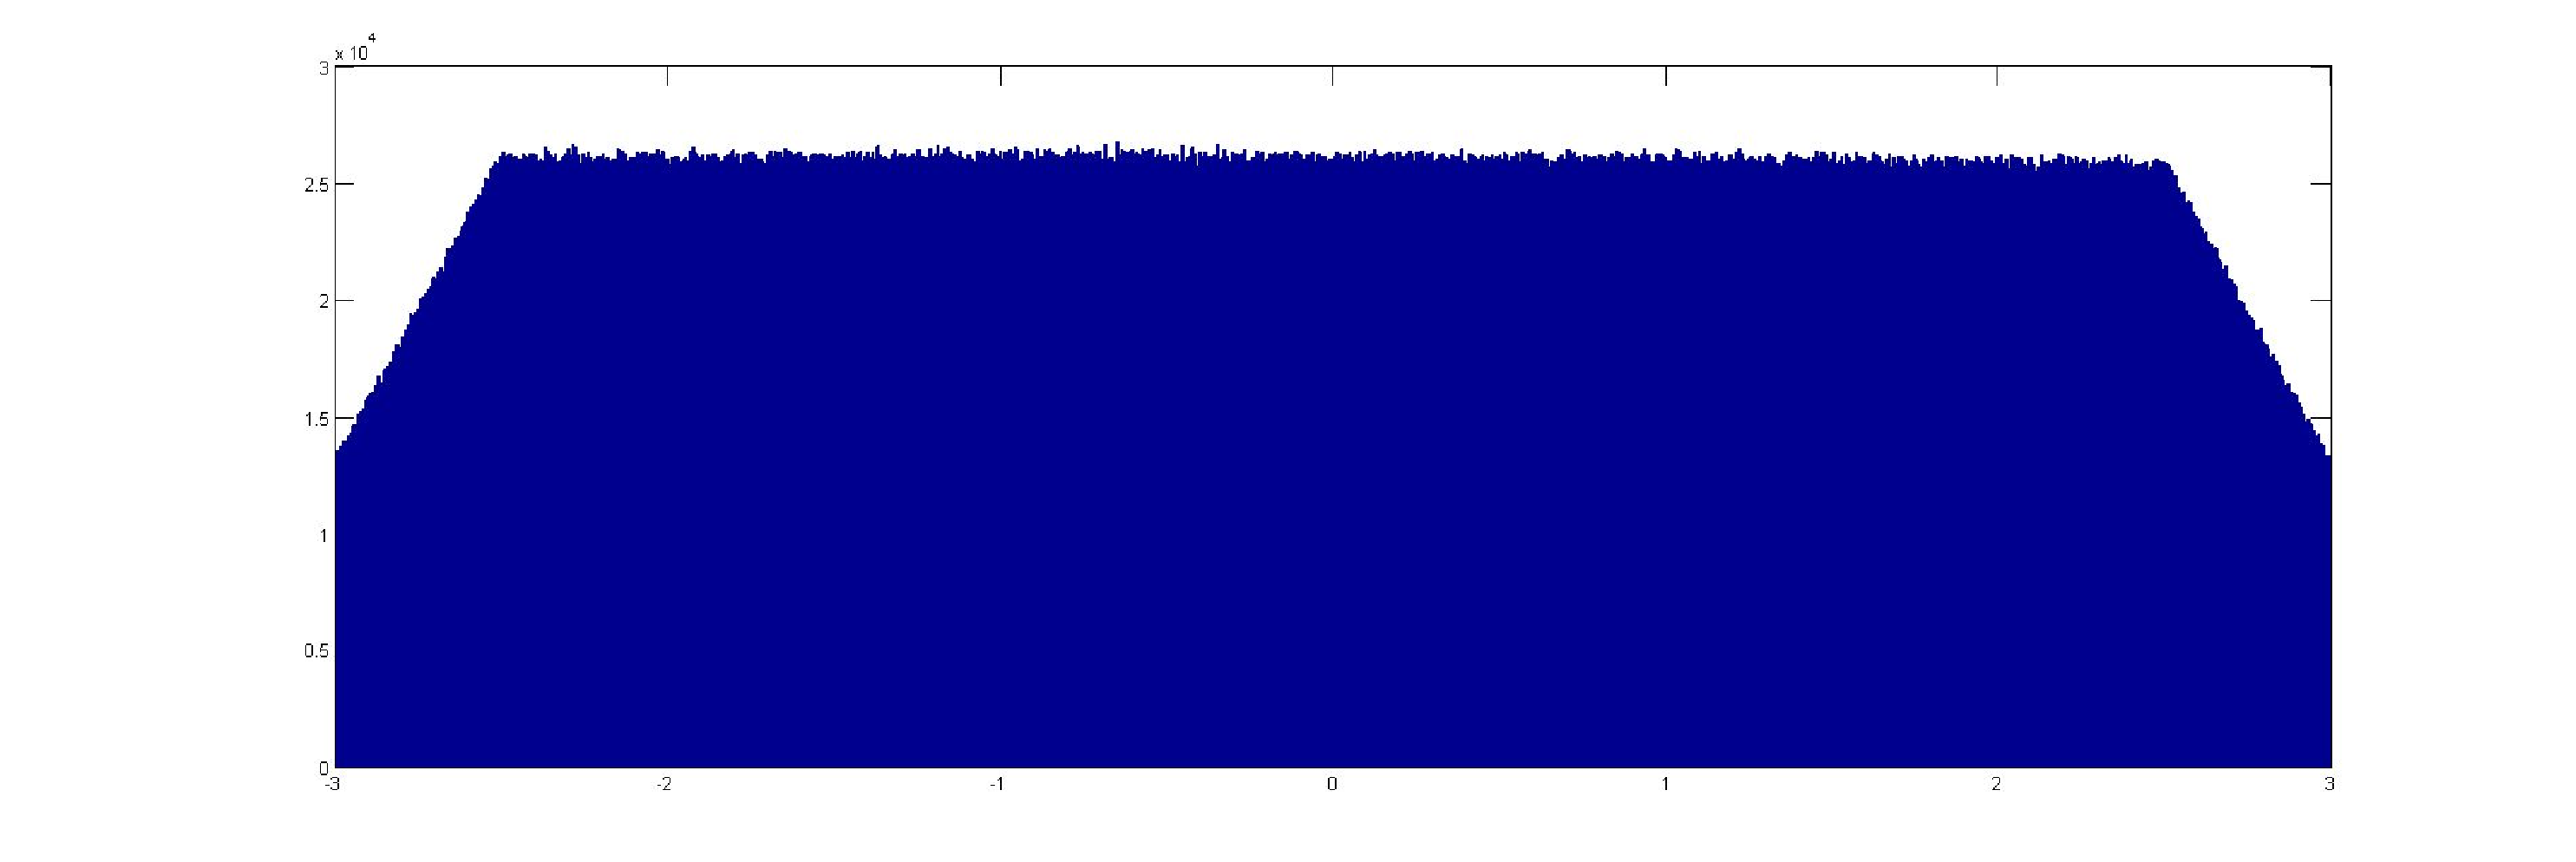
\includegraphics[width=0.45\textwidth]{s_j_20M_1__3_3}}
\caption{Histogram wystąpień punktów; metoda naprawy poprzez powtórną generację; 1 wymiar}
\end{figure}

\begin{figure}[H]
\centering
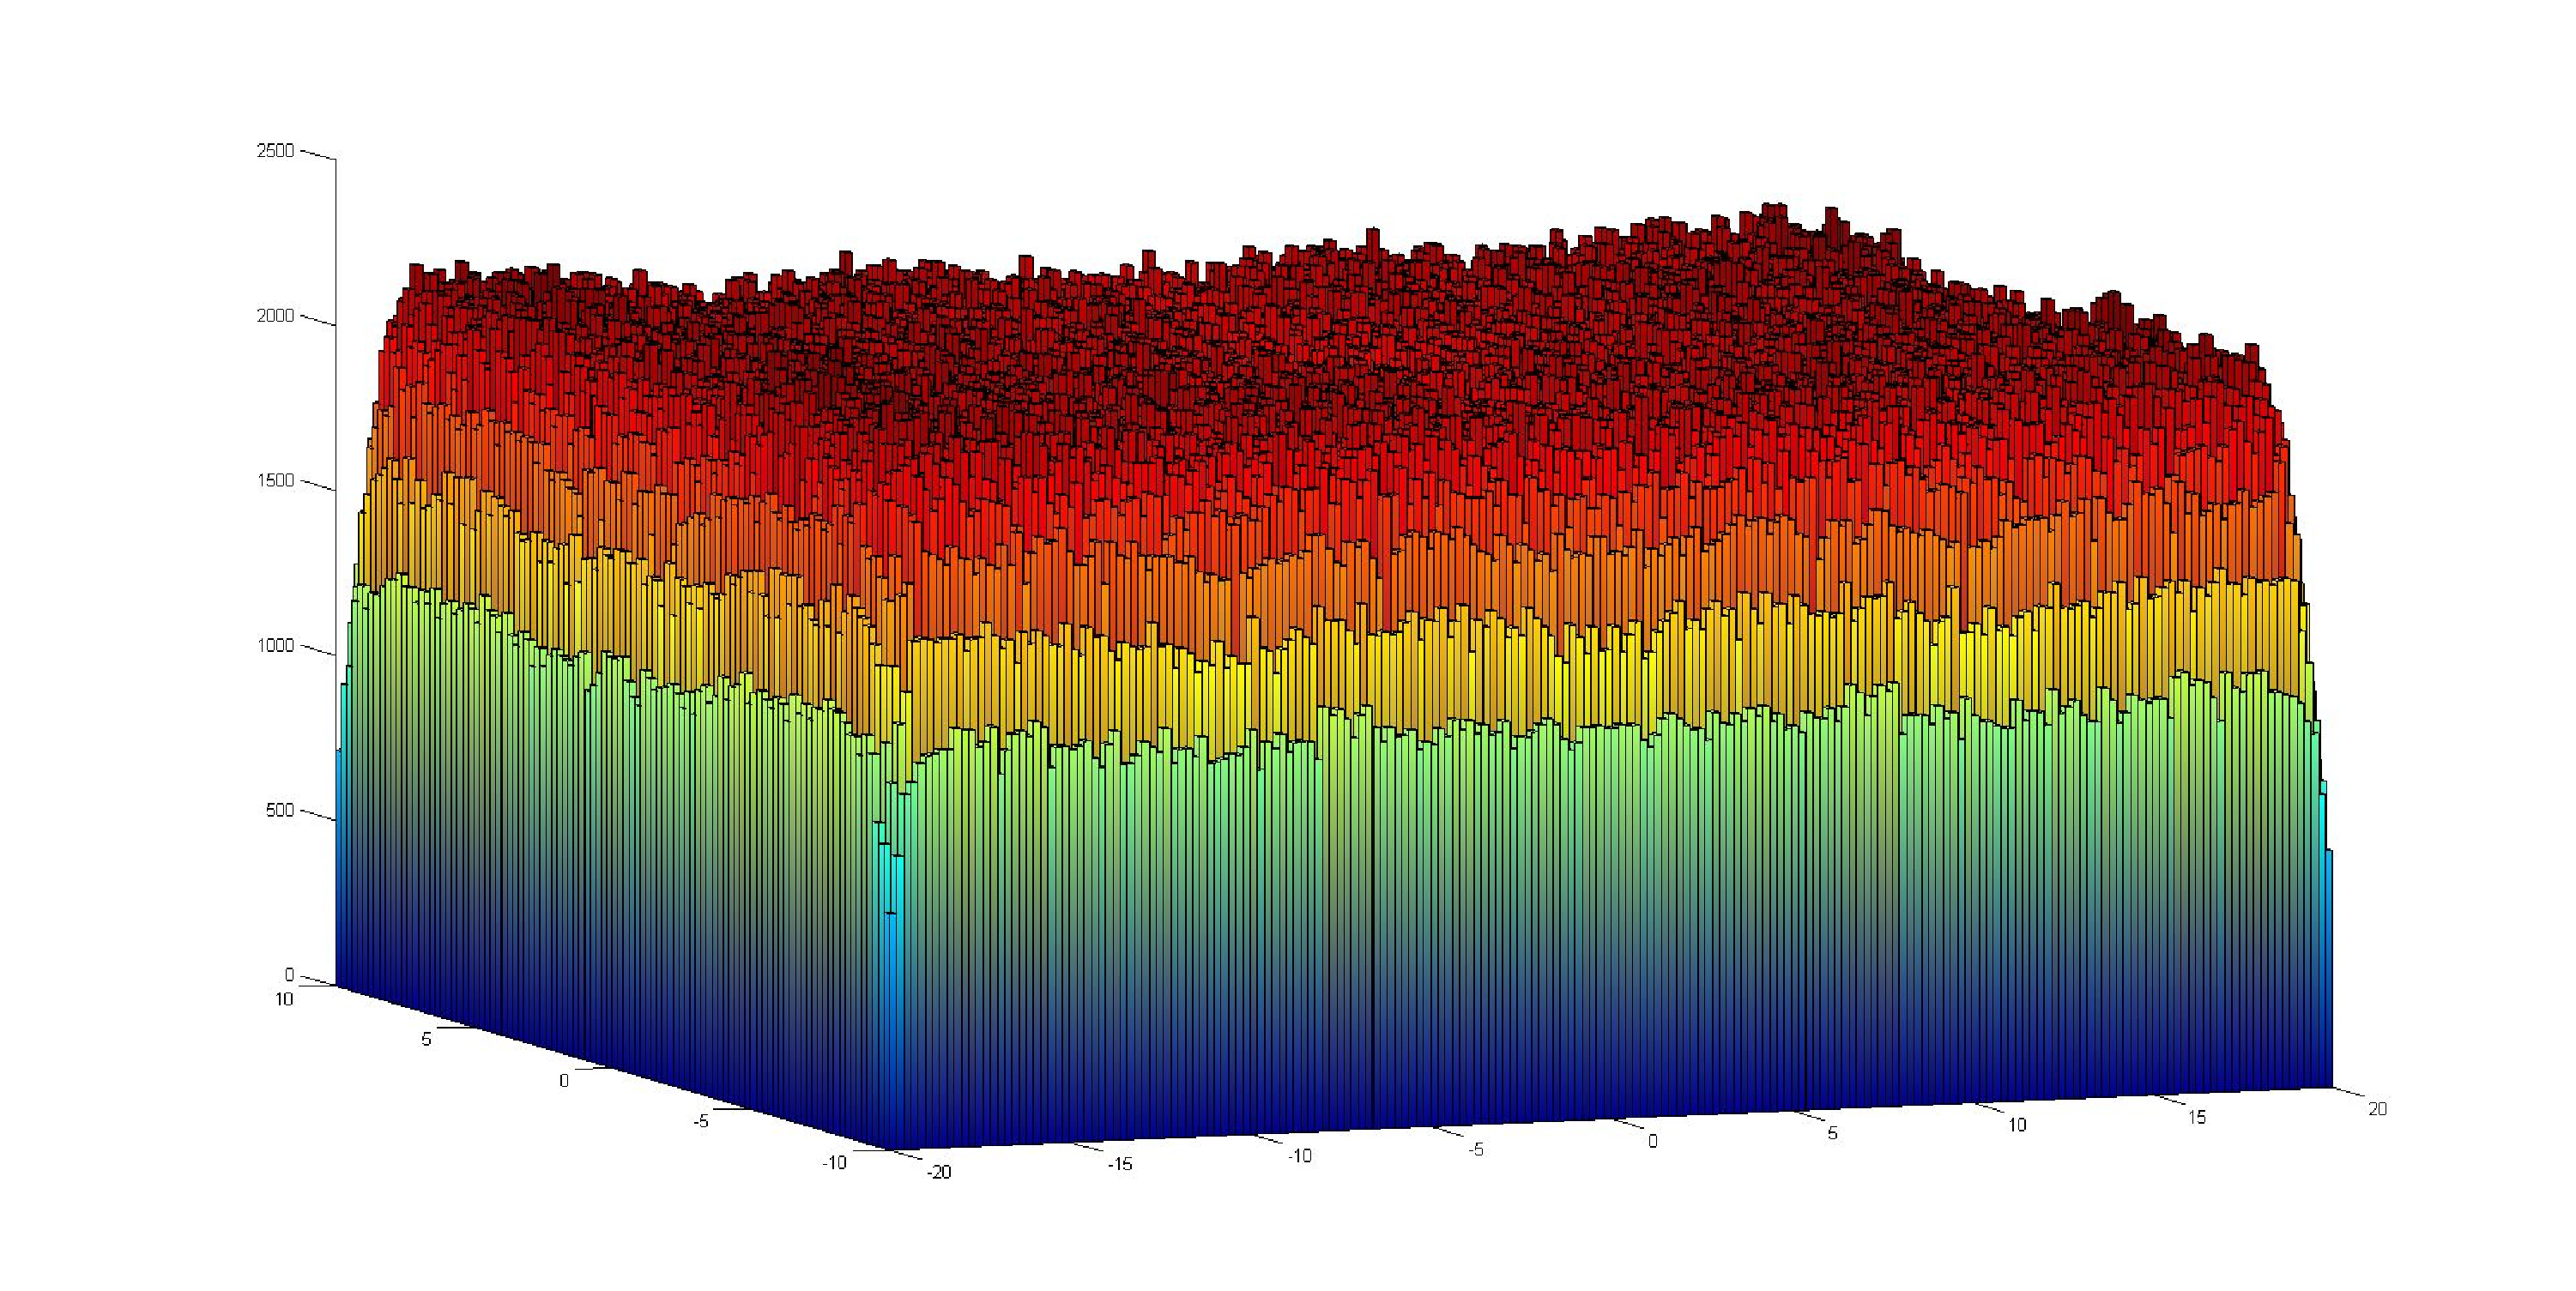
\includegraphics[width=\textwidth]{s_n_10M_2__20_20__10_10_4_2}
\caption{Histogram wystąpień punktów; metod naprawy poprzez powtórną generację; 2 wymiary; generowanie z rozkładem normalnym}
\end{figure}

\subsubsection*{Zawijanie}
\hspace{3,4ex}Wykres przesunięć wartości oczekiwanych jest bardzo nieczytelny. Jest to implikacją dużych przesunięć punktów - te, które znajdą się poza ograniczeniem, wędrują na drugą stronę wykresu.

Uzasadniając wykresy histogramów warto wyobrazić sobie, że symulacja przeprowadzana jest bez ograniczeń, a następnie wykres z wynikami przecinany jest w równych odstępach wzdłuż każdej osi. Na koniec tak pocięte części łączone są w jeden wykres. Takie zachowanie symuluje zawijanie. W związku z tym nie dziwi fakt, że histogramy przedstawiają rozkład jednostajny.

\begin{figure}[H]
\centering
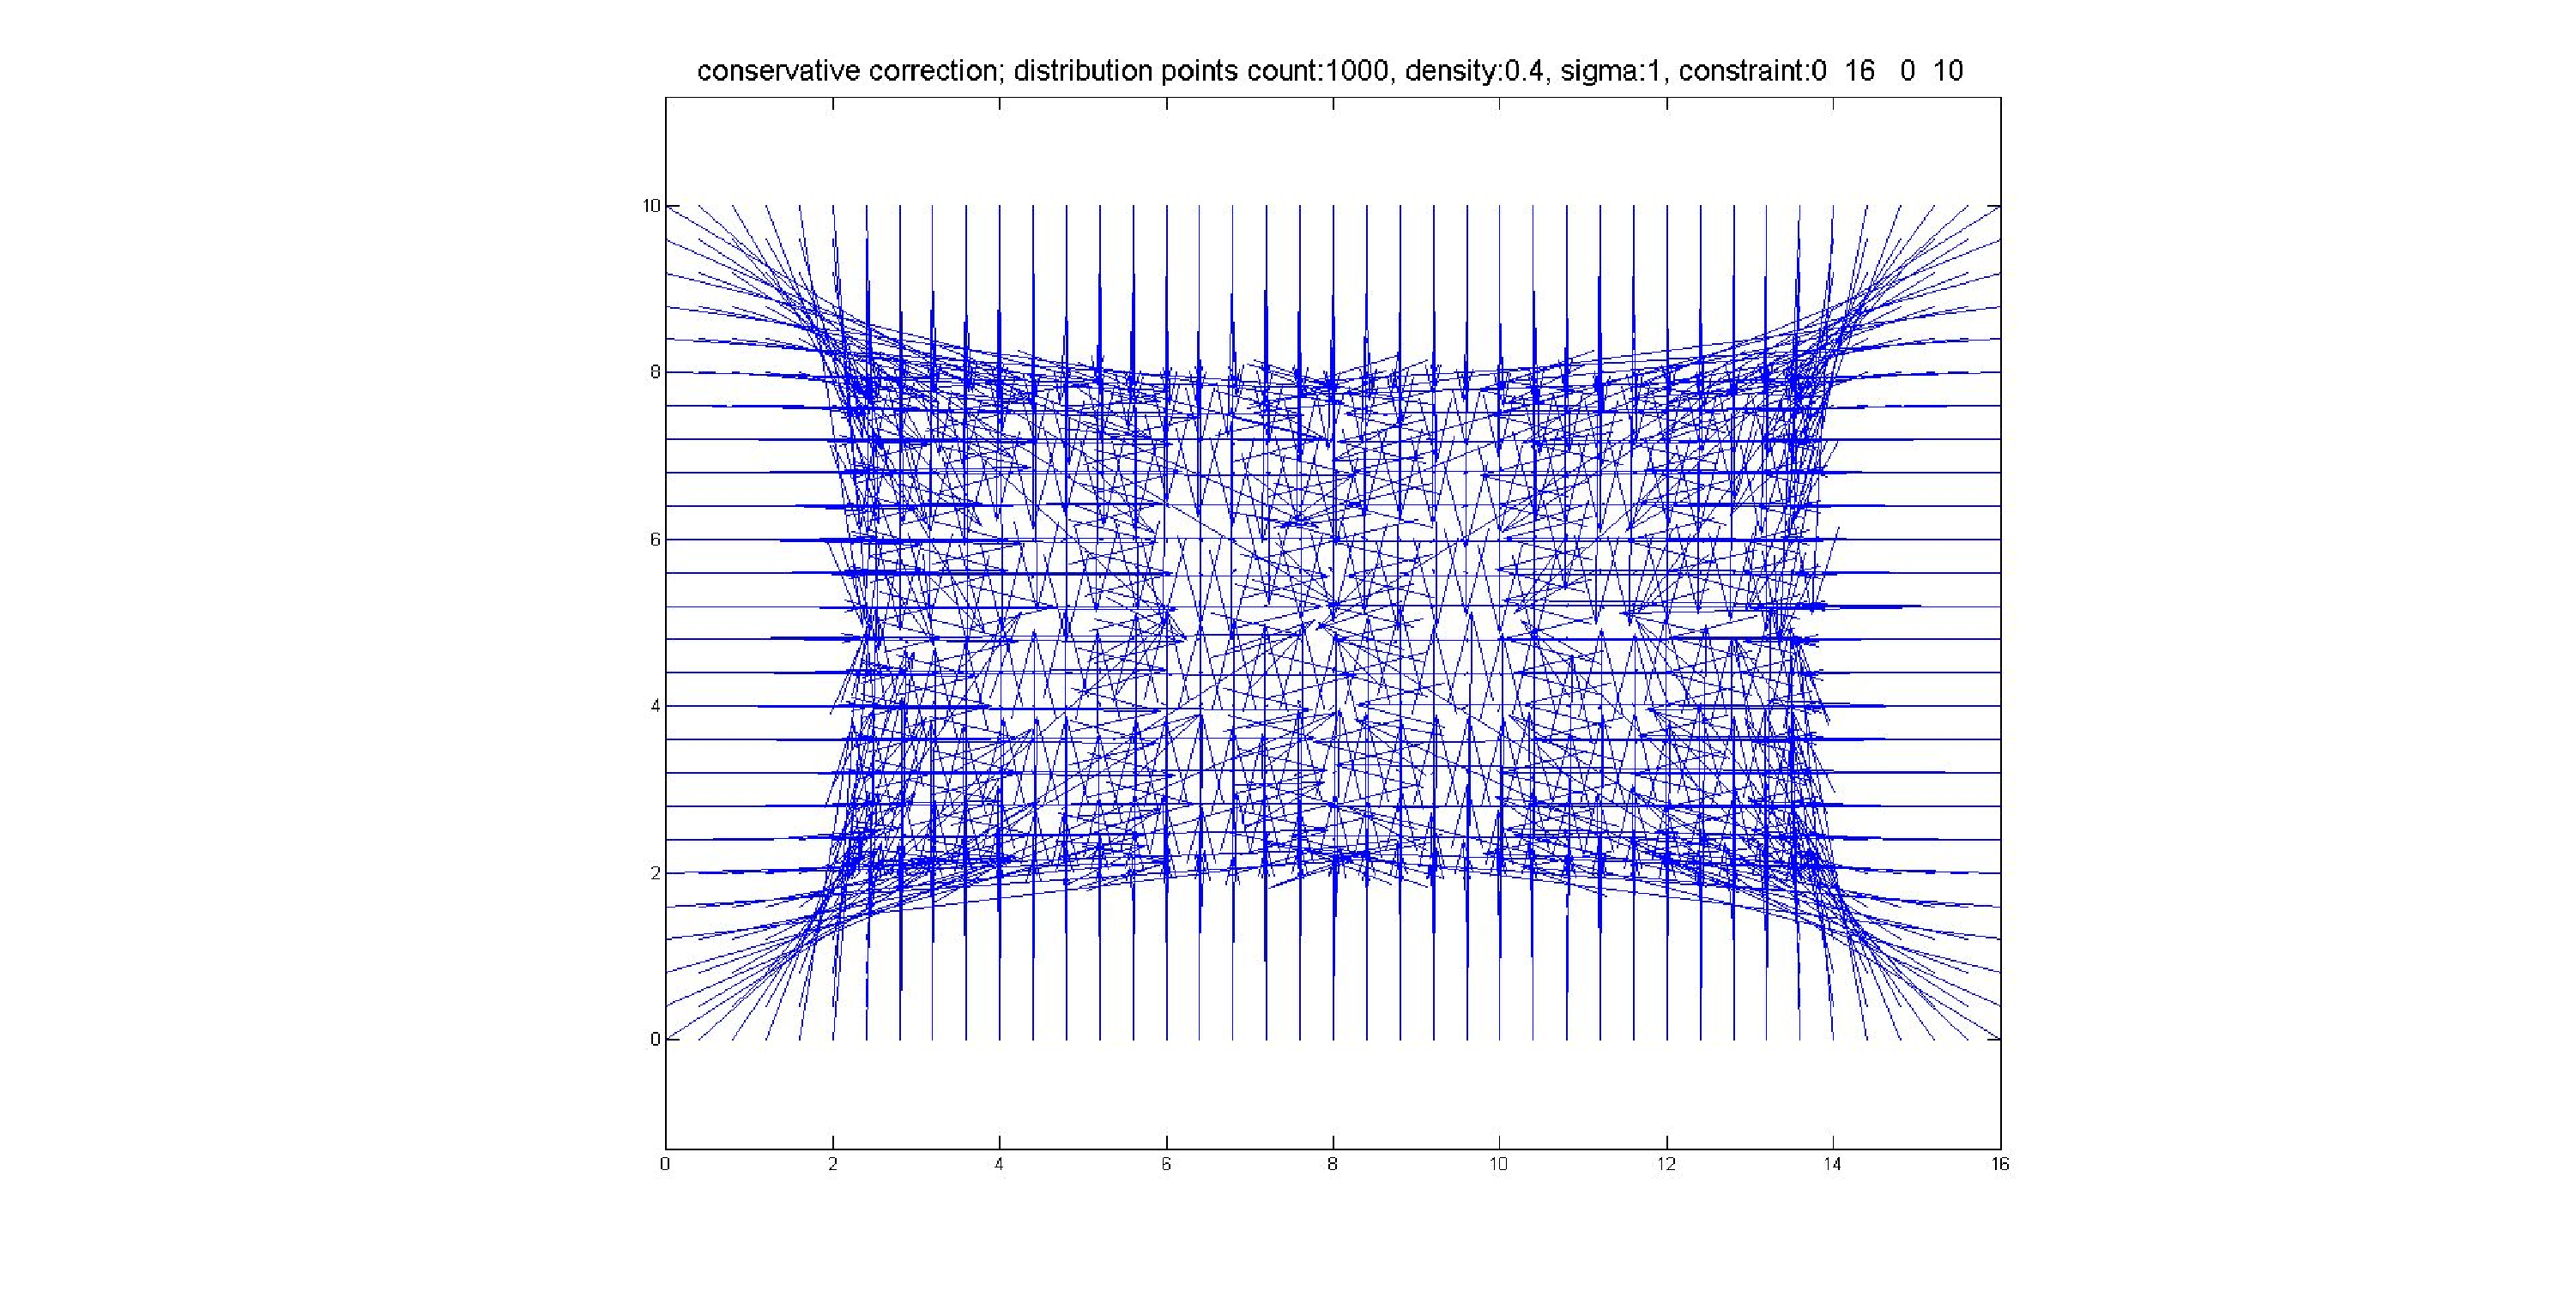
\includegraphics[width=\textwidth]{wrapping2dprzesuniecie}
\caption{Wykres wektorów przesunięć wartości oczekiwanych dla naprawy poprzez zawijanie}
\end{figure}

\begin{figure}[H]
\centering
\subfloat[1 wymiar; generowanie z rozkładem normalnym]{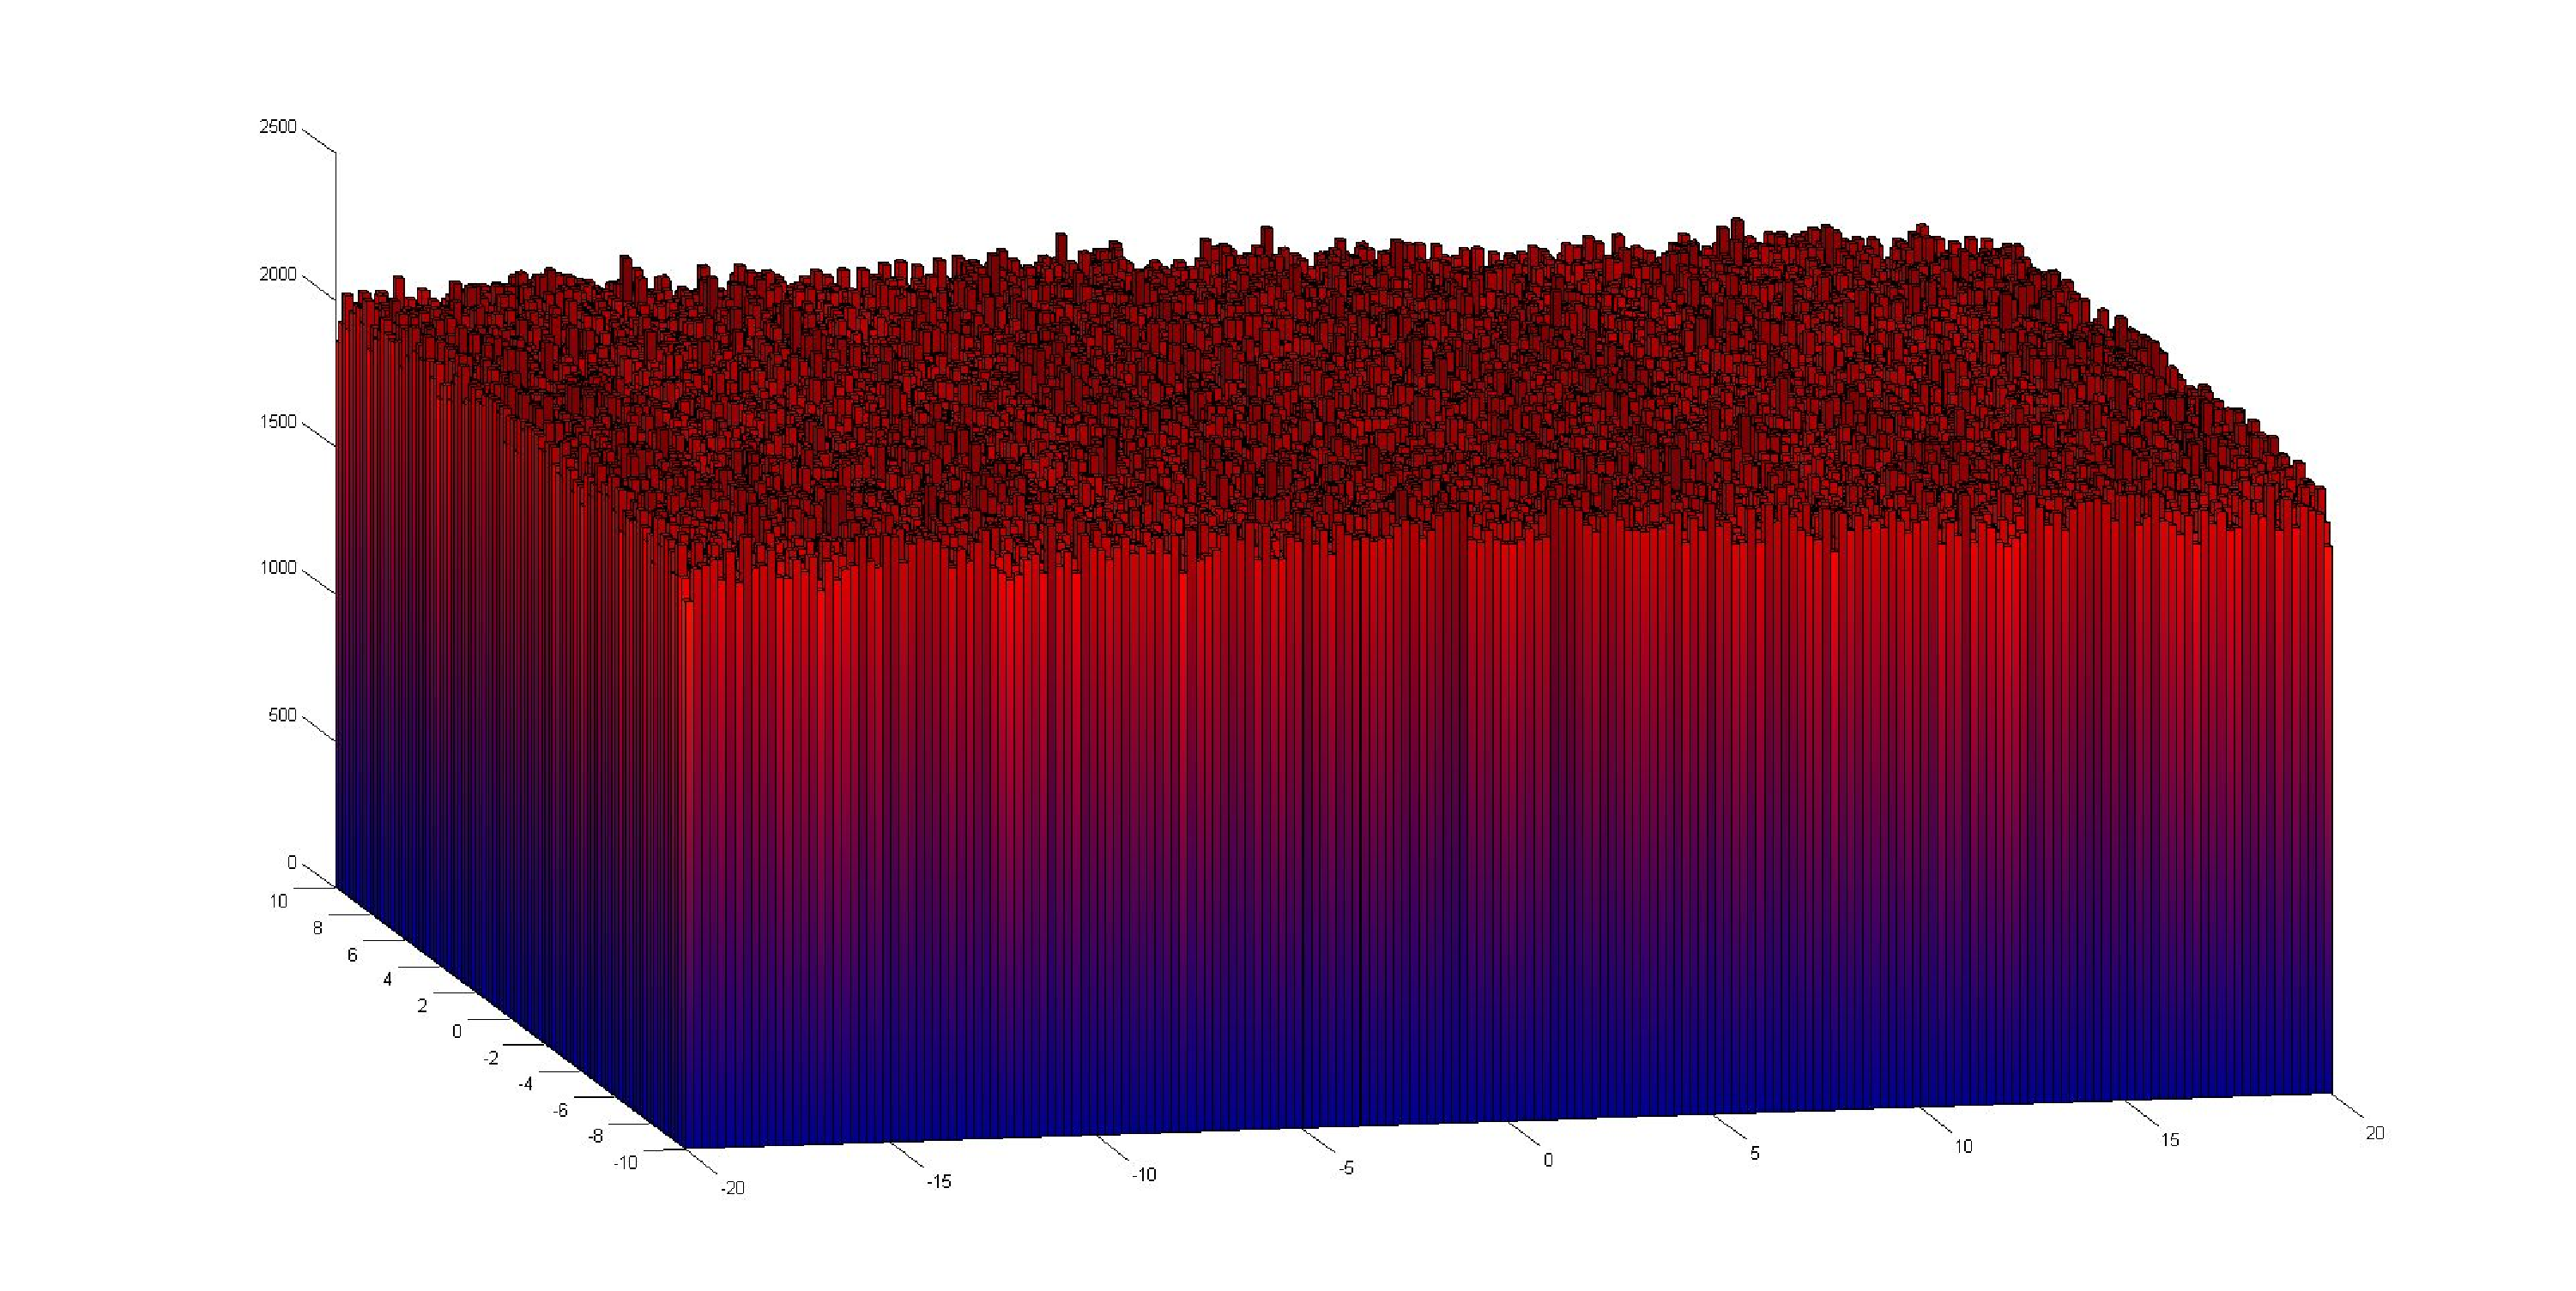
\includegraphics[width=0.45\textwidth]{w_n_10M_2__20_20__10_10_4_2}}
\quad
\subfloat[2 wymiary; generowanie z rozkładem jednostajnym]{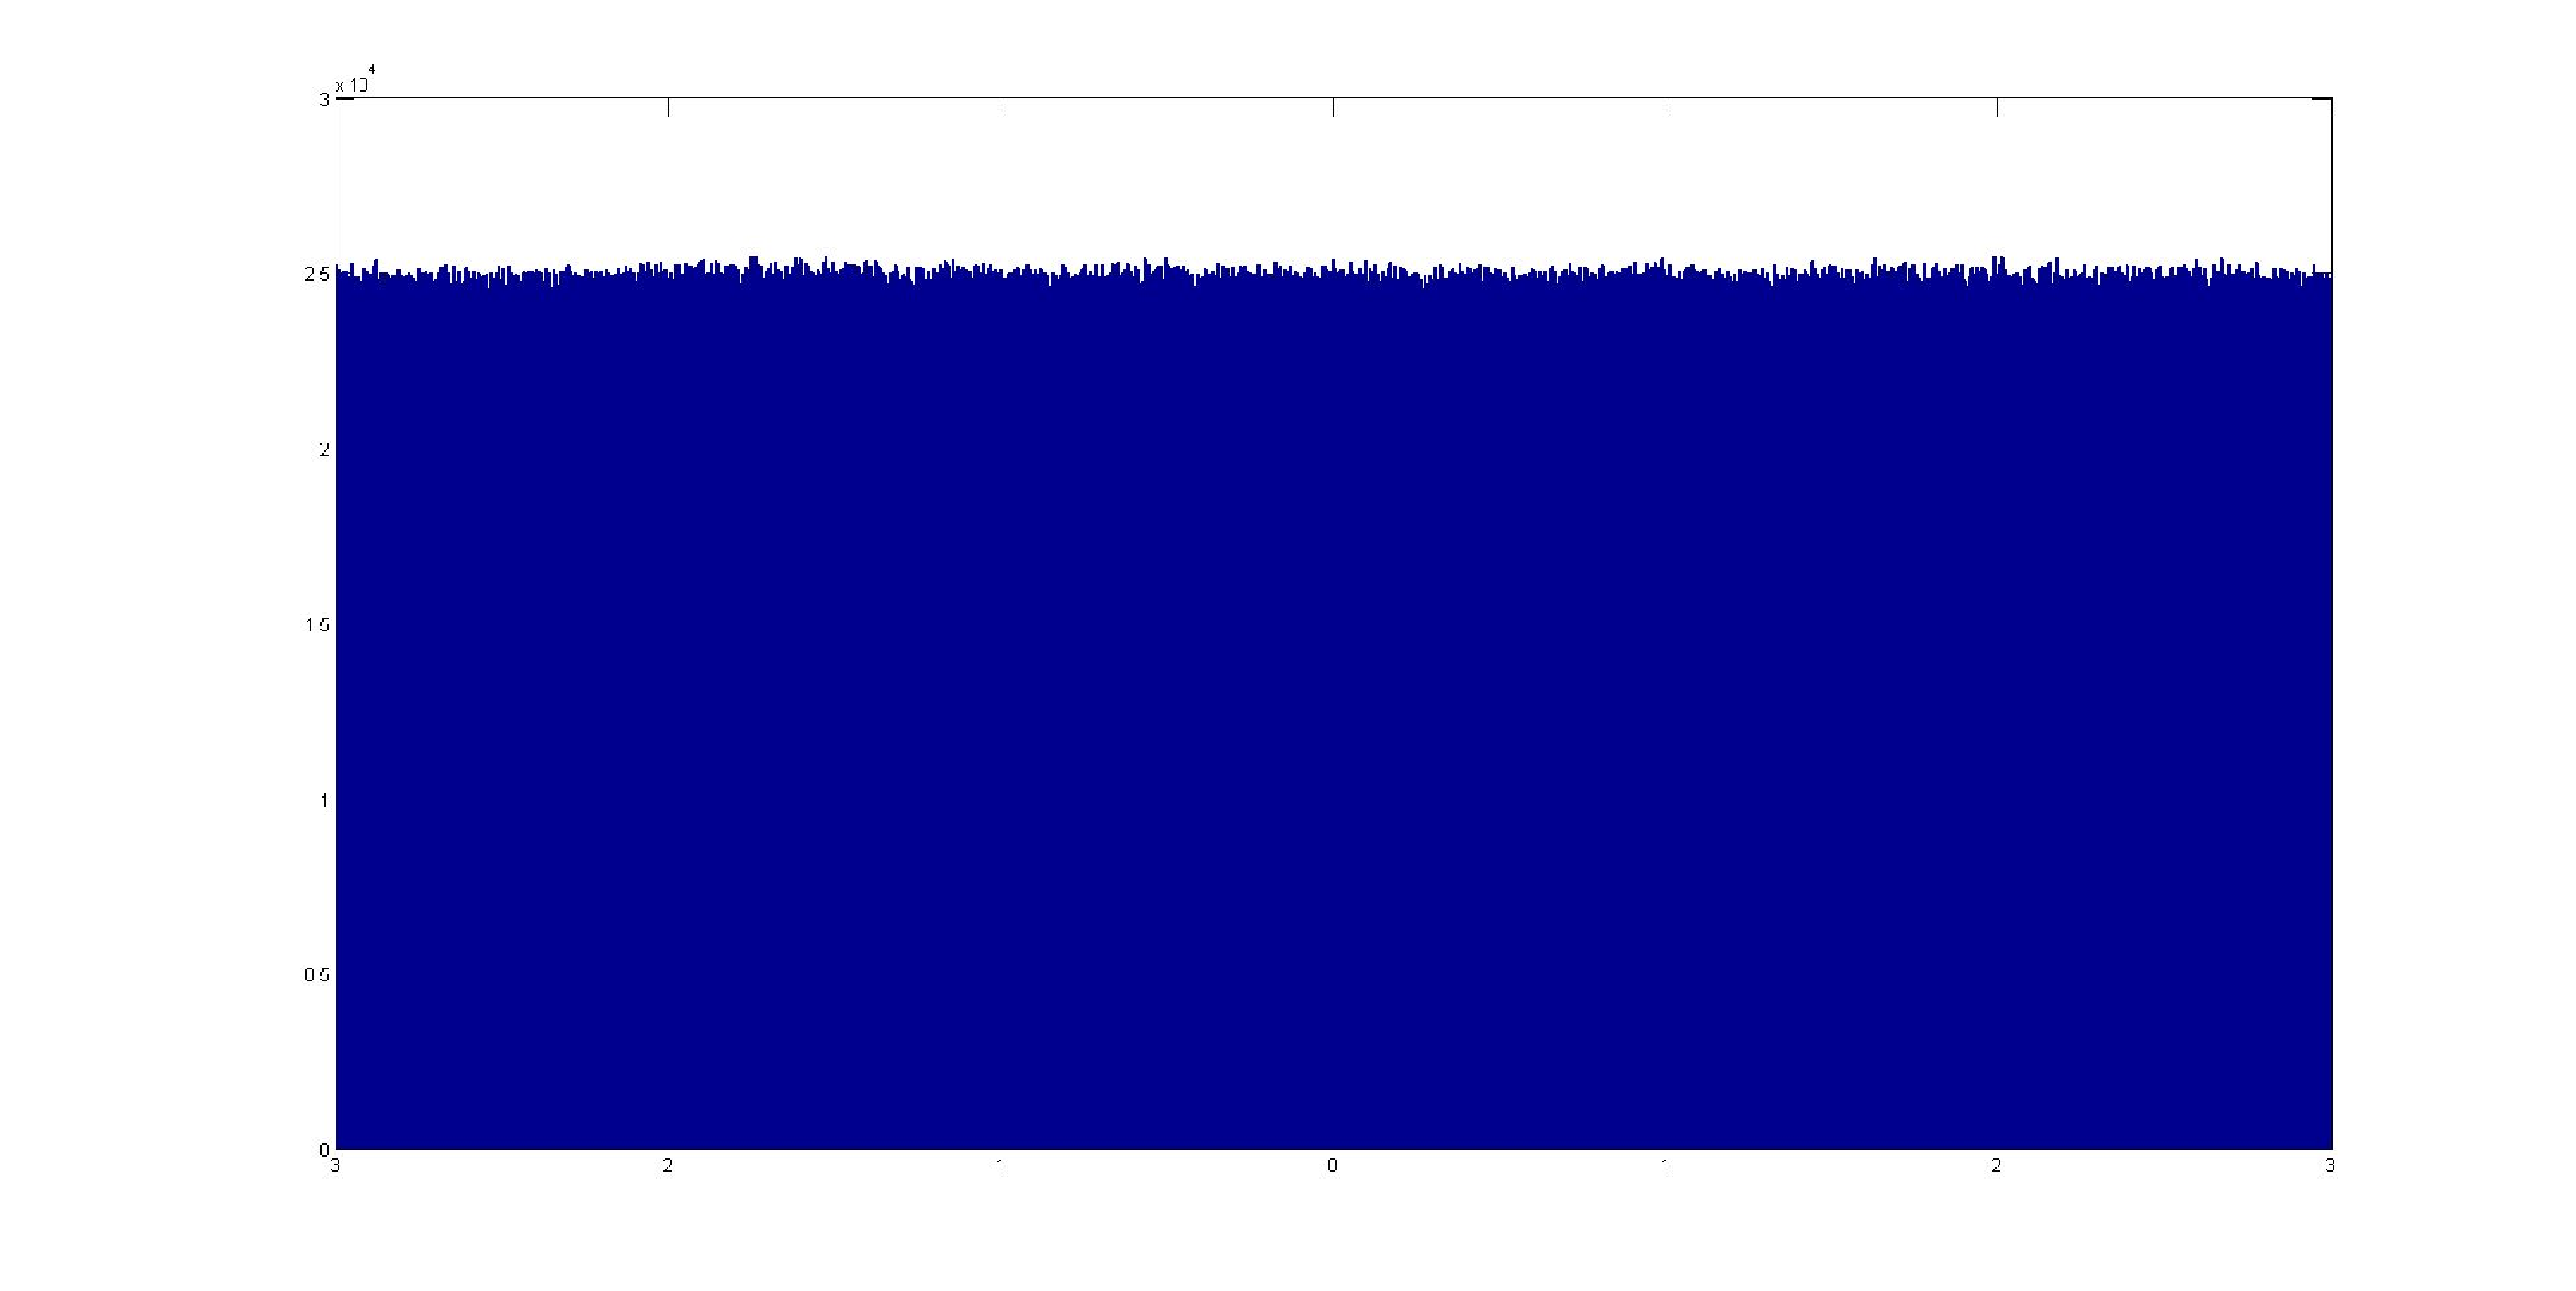
\includegraphics[width=0.45\textwidth]{w_j_20M_1__3_3}}
\caption{Histogram wystąpień punktów; naprawa poprzez zawijanie}
\end{figure}

\subsubsection*{Odbicie}
\hspace{3,4ex}Podobnie jak zawijanie, odbicie zwraca histogram zbliżony do rozkładu jednostajnego. W~tej sytuacji nieco trudniej o analogię, lecz po chwili zastanowienia nie dziwi kształt poniższych wykresów.

Od zawijania różni się natomiast wykres wartości oczekiwanych, ponieważ w odbiciu nie ma znaczących przesunięć punktów.

\begin{figure}[H]
\centering
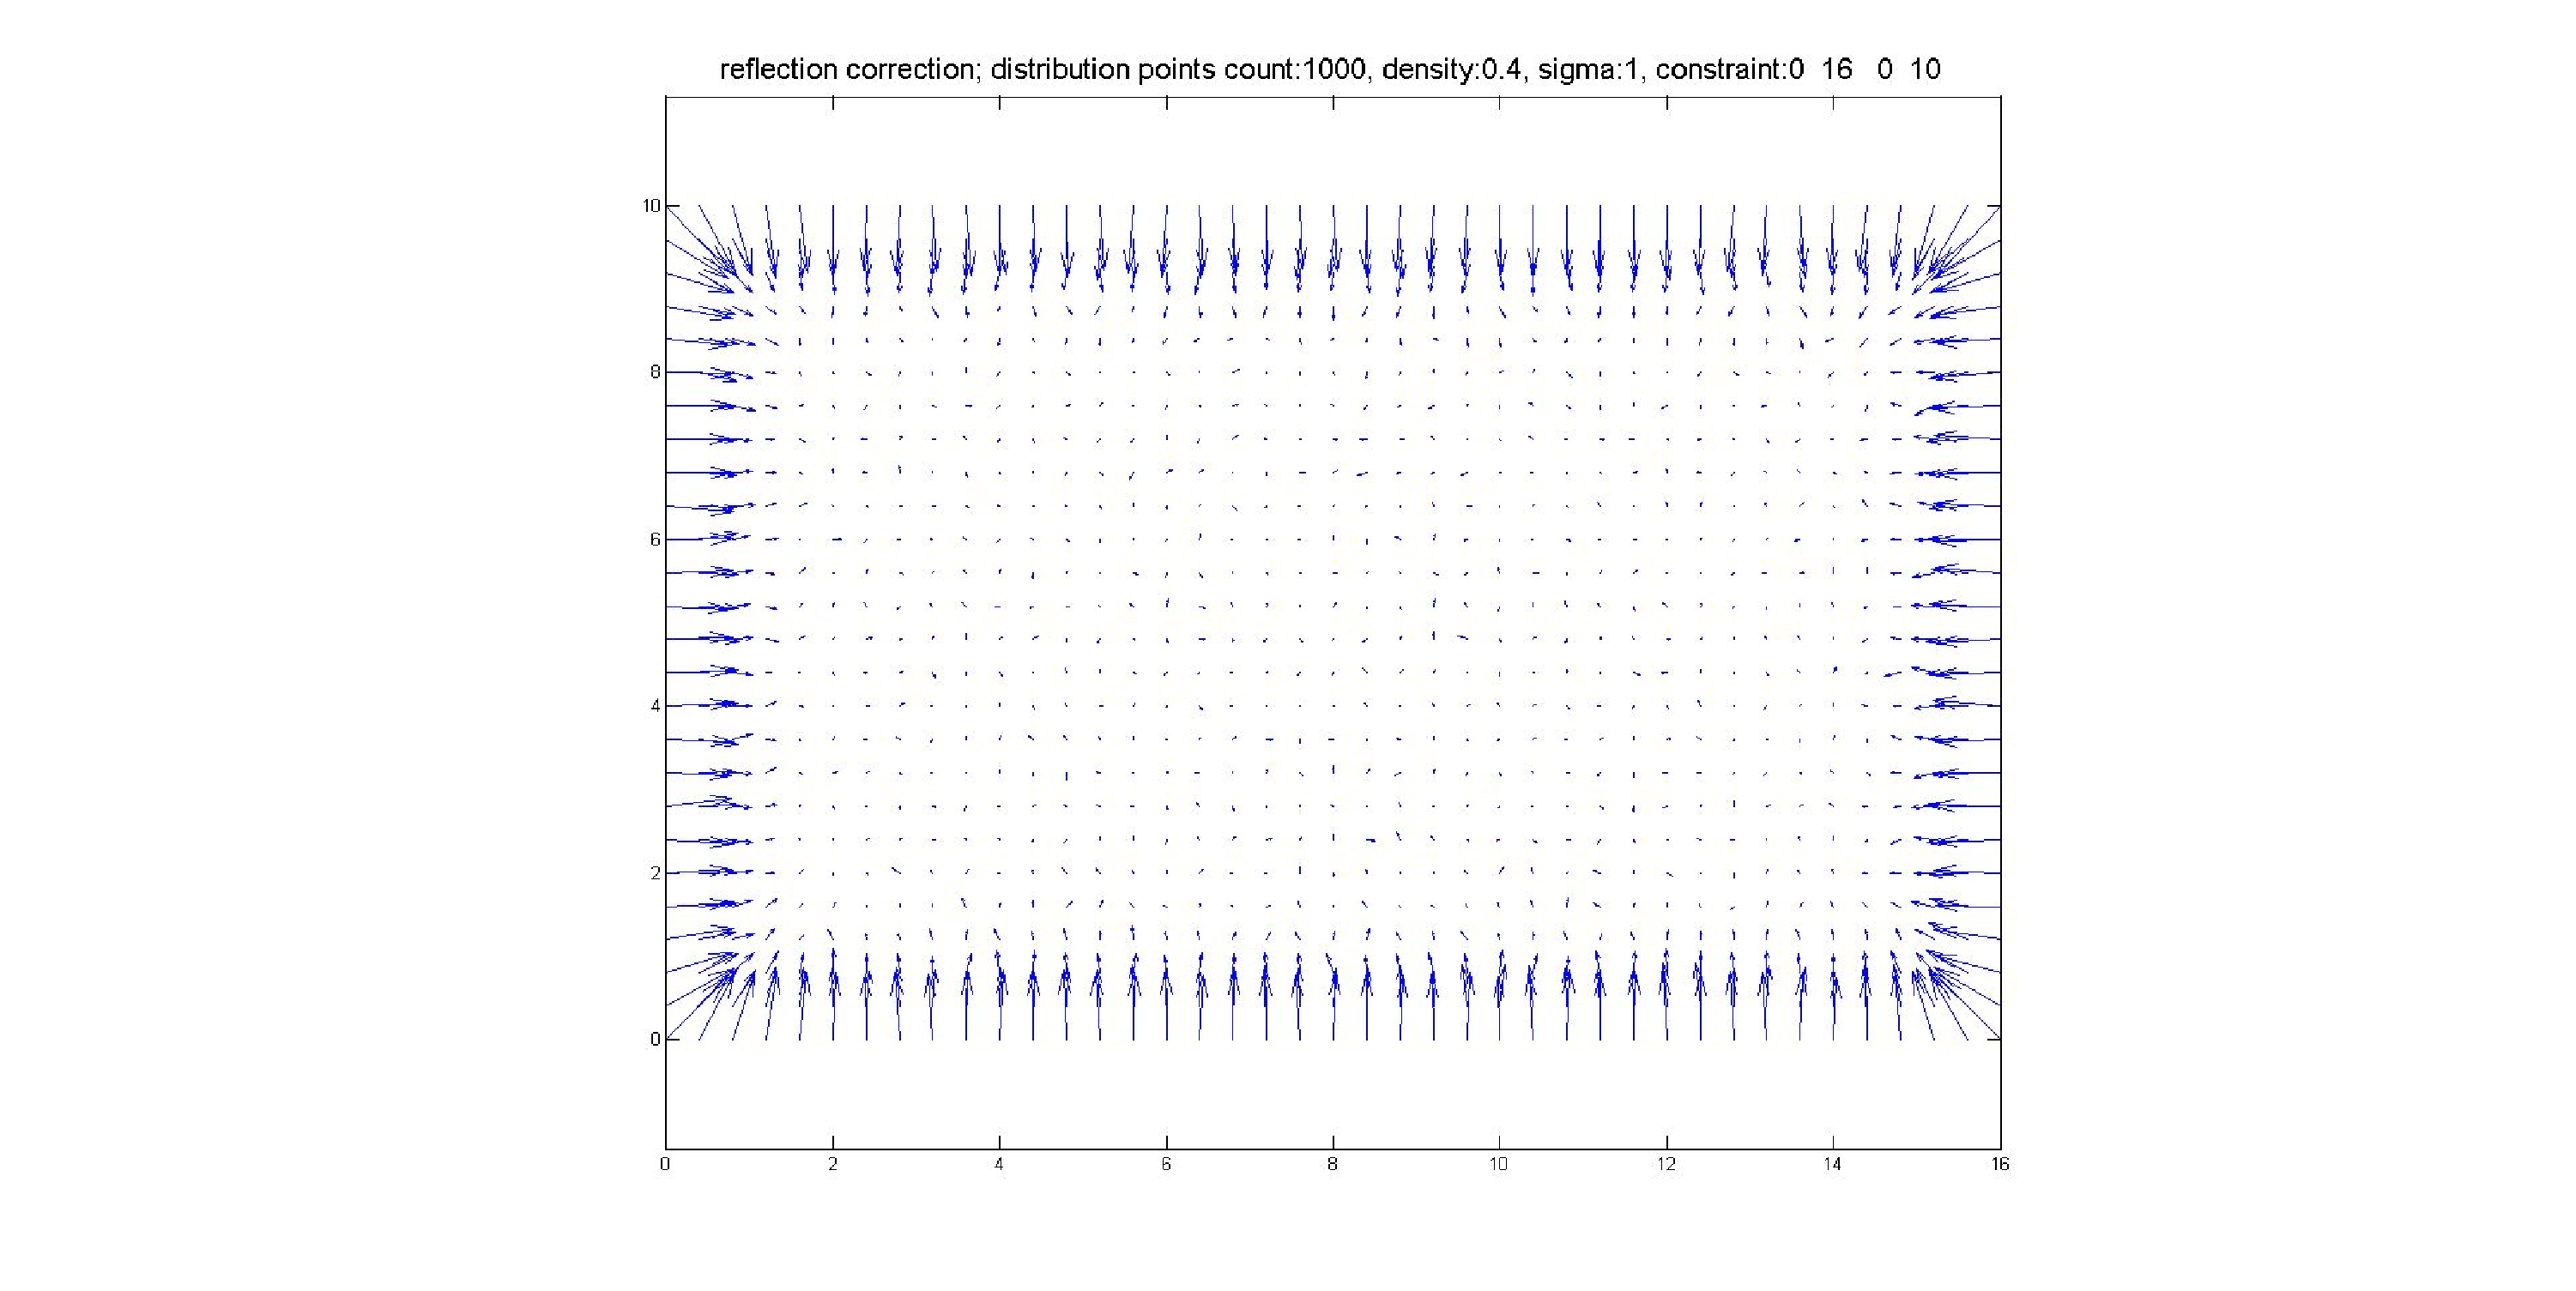
\includegraphics[width=\textwidth]{reflection2dprzesuniecie}
\caption{Wykres wektorów przesunięć wartości oczekiwanych dla naprawy poprzez odbicie}
\end{figure}

\begin{figure}[H]
\centering
\subfloat[1 wymiar; generowanie z rozkładem normalnym]{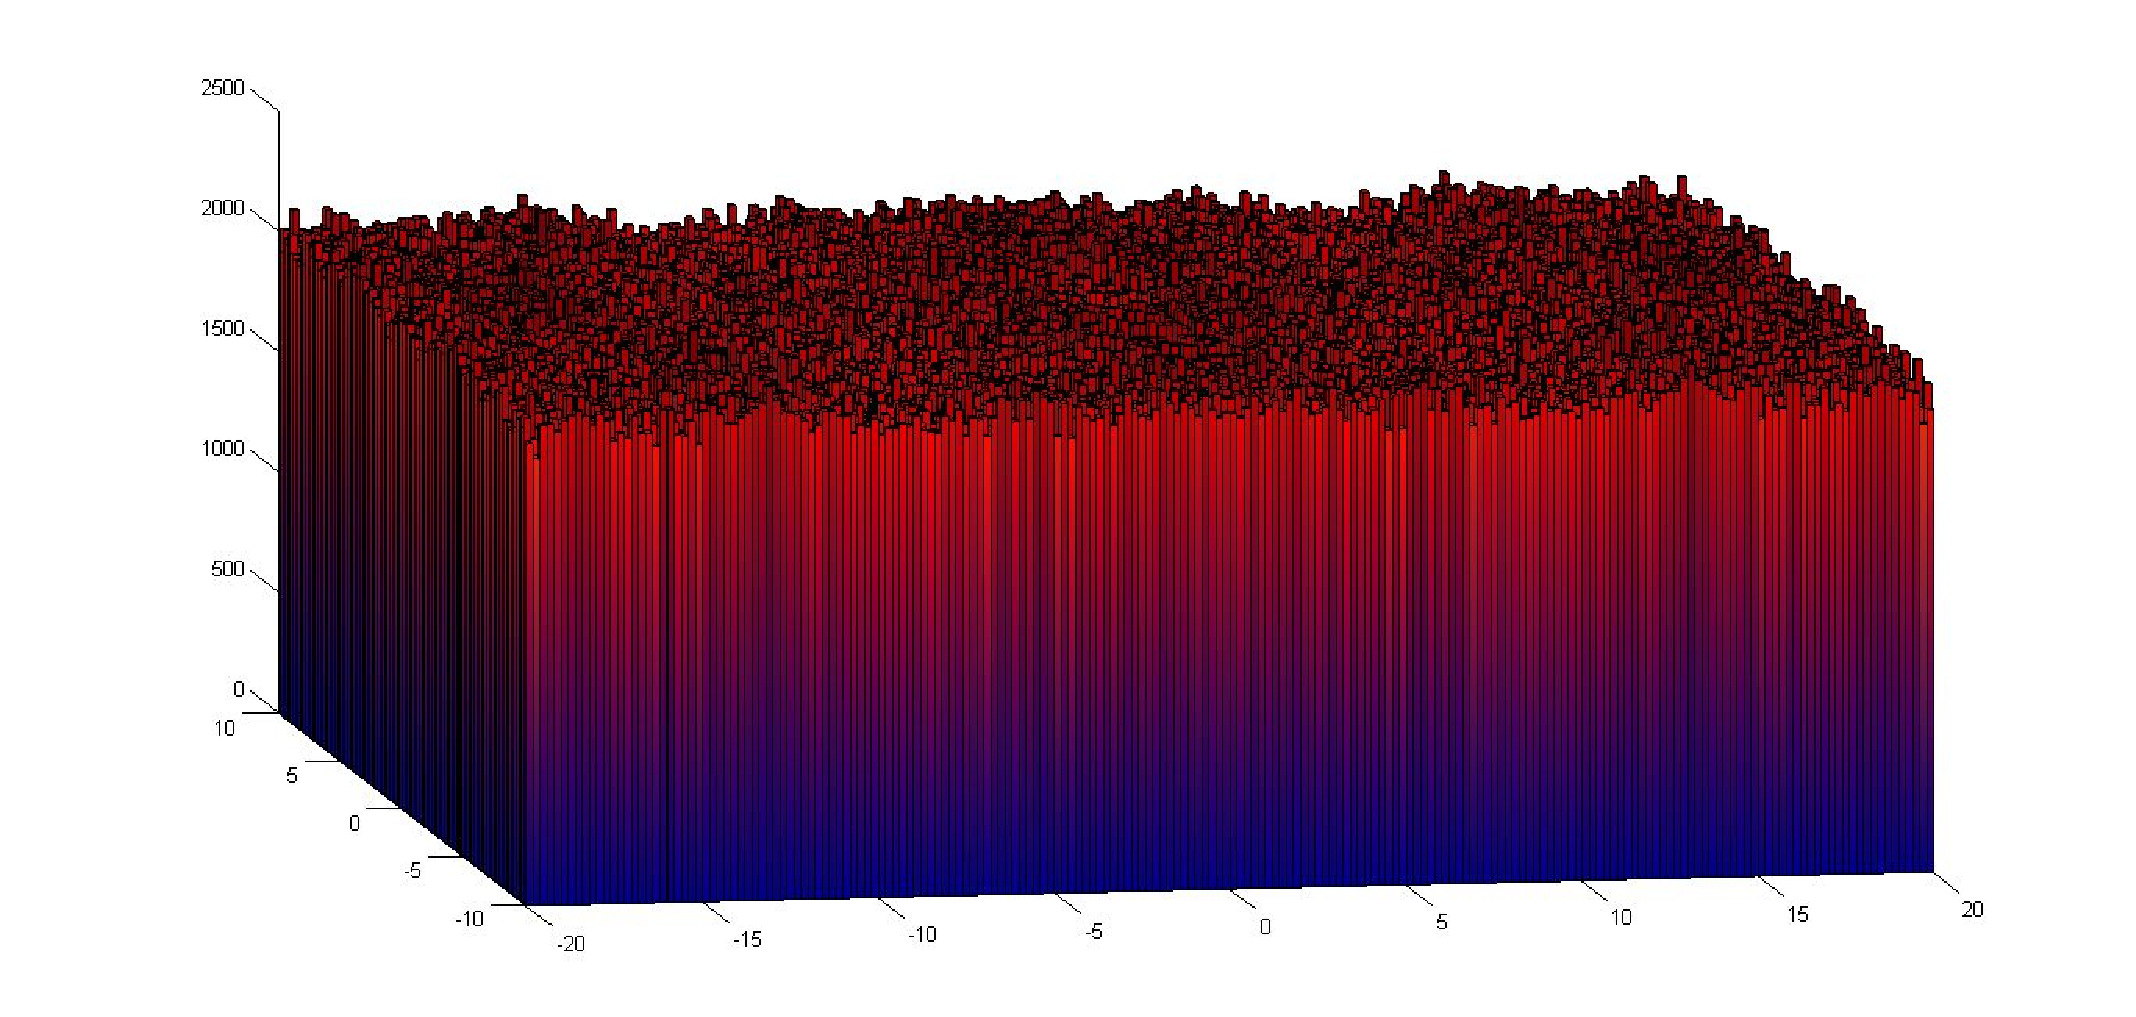
\includegraphics[width=0.45\textwidth]{rf_n_10M_2__20_20__10_10_4_2}}
\quad
\subfloat[2 wymiary; generowanie z rozkładem jednostajnym]{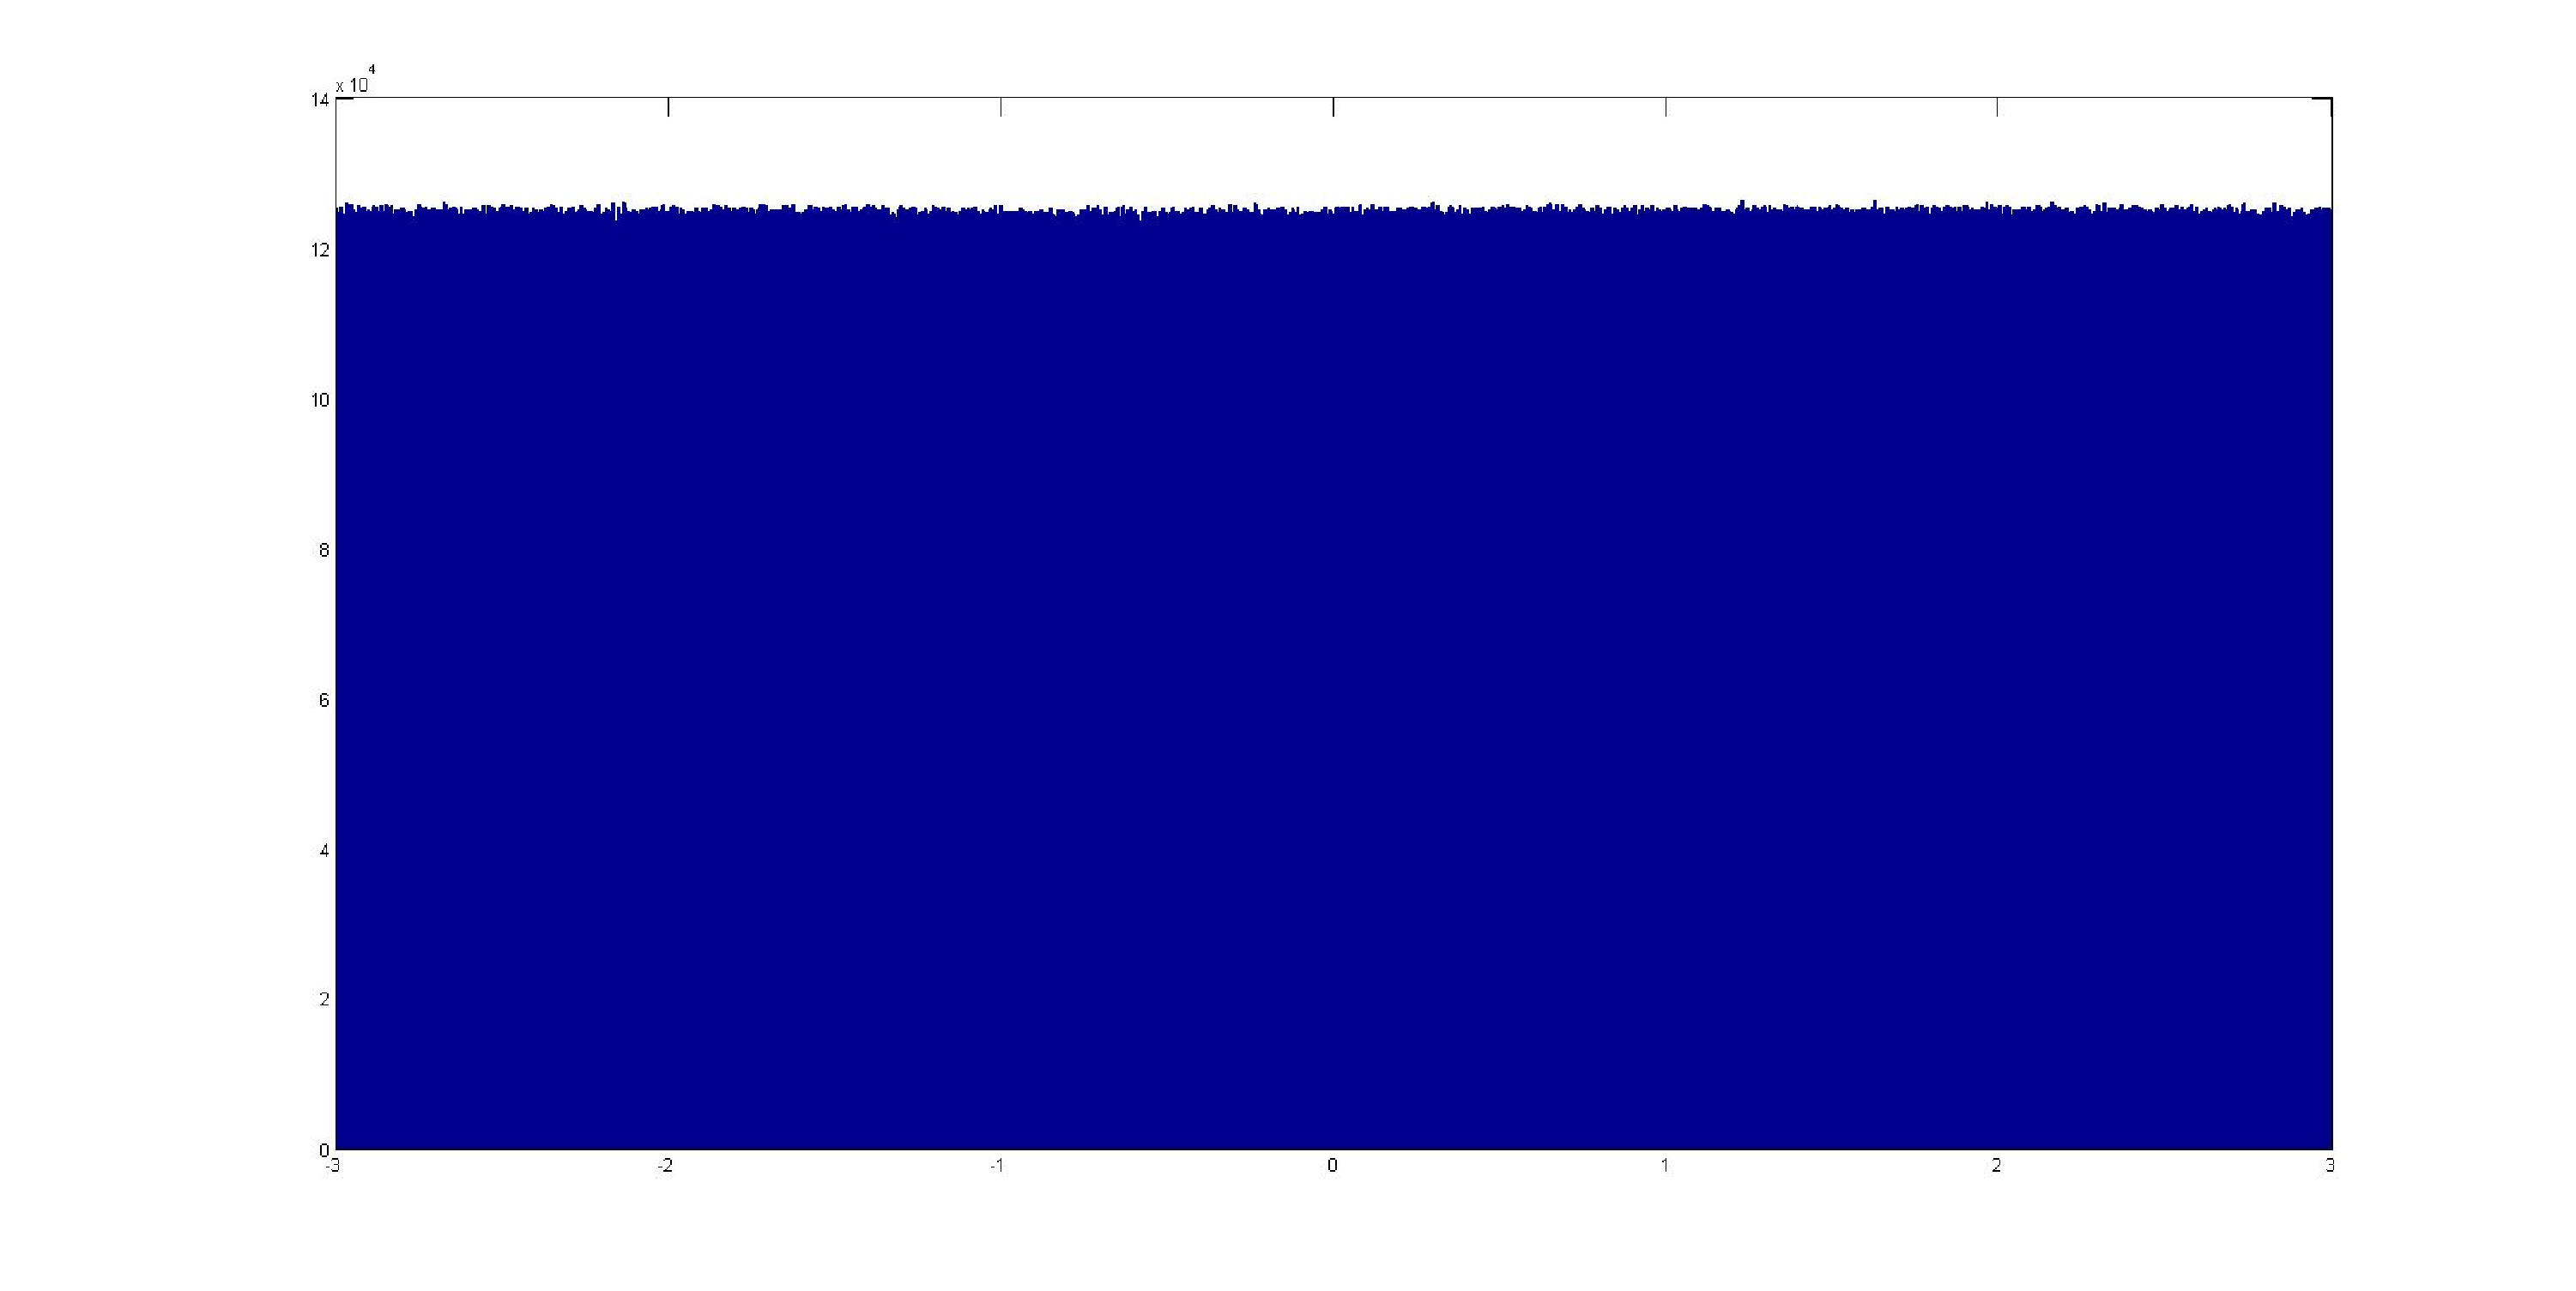
\includegraphics[width=0.45\textwidth]{rf_j_100M_1__3_3}}
\caption{Histogram wystąpień punktów; naprawa poprzez odbicie}
\end{figure}

\subsection{Wnioski}
\hspace{3,4ex}W większości metod zachowanie pojedynczego punktu przekłada się na globalne zachowanie całego algorytmu. Testy pokazały cechy, które nie były oczywiste podczas prostej analizy algorytmów.

Z perspektywy algorytmu CMA-ES warto zwrócić uwagę przede wszystkim na metody zawijania i reinicjacji. W tych metodach wartości oczekiwane punktów znajdują się daleko od rodzica. Oznacza to, że w algorytmie CMA-ES macierz kowariancji może znacząco się zniekształcać w porównaniu do metod bez ograniczeń.

\pagebreak

\section{Metodyka testowania metod optymalizacji globalnej}
\hspace{3,4ex}Funkcje celu posiadają charakterystyczne cechy, m.in. monotoniczność, liczba ekstremów, ciągłość. Metody optymalizacji globalnej również posiadają swoje charakterystyczne własności. W zależności od przypadku, wymagania stawiane algorytmowi mogą być różne: szybkość działania, czy też dokładne określenie ekstremum. Połączenie tego wszystkiego powoduje, że trudno jednoznacznie określić, która metoda optymalizacji jest najlepsza. Warto jednak posiadać wiedzę w których przypadkach metoda przynosi lepsze rezultaty.

Zapewne zgodziliby się z tym stwierdzeniem twórcy konkursów takich jak CEC, czy BBOB. Tworzą oni szereg zbiorów funkcji benchmarkowych, które mają na celu empirycznie pokazać silne i słabe strony algorytmów w konkretnych sytuacjach.

Zbiory te zawierają zarówno funkcje jednomodalne, jak i wielomodalne o różnym stopniu komplikacji. Skomplikowanie polega między innymi na wielu ekstremach funkcji lub specyficznym umieszczeniu minimum globalnego. Dzięki nim można porównać algorytmy.

Wybranie funkcji benchmarkowych nie wystarczy, aby stwierdzić, który z algorytmów ewolucyjnych jest lepszy. Są to algorytmy niedeterministyczne - poszukiwanie rozwiązania za każdym razem będzie wyglądało inaczej nawet przy takich samych parametrach. Oznacza to, że dla wiarygodności wyników należy testy uruchamiać wielokrotnie. Posiadając takie wyniki należy posłużyć się wybraną metodą, aby porównać skuteczność algorytmów. W tej pracy do porównywania został wybrany test Wilcoxona, ponieważ można go użyć do porównywania par obserwacji.

Test Wilcoxona jest testem nieparametrycznym - nie jest potrzebna wiedza na temat rozkładu populacji \cite{wilcox}. Ten test sprawdza, czy istnieje statycznie istotna różnica między dwoma zbiorami, które były losowane z pewnym rozkładem prawdopodobieństwa. Hipoteza dotyczy median wygenerowanych zbiorów. Hipoteza zerowa $H_0$ brzmi "Różnica median zbiorów wynosi 0". Na podstawie sprawdzenia hipotezy możemy wywnioskować, czy dwa rozkłady prawdopodobieństwa generują dane istotnie różne.

Do przedstawienia wyników wielu testów Wilcoxona wykorzystuje się tabele. Taka tabela zazwyczaj zawiera etykiety porównywanych zbiorów w wierszach i kolumnach, a na przecięciach znajduje się wynik testu.

\pagebreak

\section{Weryfikacja wpływu technik uwzględniania ograniczeń na efektywność CMA-ES}

\subsection{Cel testów}
\hspace{3,4ex}Zrealizowanie celu całej pracy wymaga sprawdzenia wpływu ograniczeń kostkowych na algorytm \CMAES. Niemożliwe jest zrealizowanie tego celu bez przetestowania samego algorytmu.

Celem testów będzie sprawdzenie charakterystycznych zachowań macierzy kowariancji. Aby zrealizować ten cel, zostaną przeprowadzone testy, które sprawdzają rozkład prawdopodobieństwa punktów. Porównana zostanie także skuteczność algorytmu CMA-ES w zależności od sposobu uwzględniania ograniczeń.

Przeprowadzone zostały dwa testy. W pierwszym z nich uruchamiano jednorazowo algorytm CMA-ES z różnymi modyfikacjami zbierając położenia generowanych punktów. Drugi test polegał na wielokrotnym uruchomieniu każdej z przygotowanych modyfikacji. Wyniki symulacji zostały porównane testem Wilcoxona.

Testy zostały oparte na bibliotece przygotowanej przez Nikolausa Hansena. Tak jak w przypadku błądzenia przypadkowego, wykorzystano implementację w języku MATLAB \cite{cmaes_code}. Wspomniana biblioteka była modyfikowana w celu zrealizowania testów.

\subsection{Ilustracja zbioru punktów generowanych przez algorytm CMA-ES z użyciem różnych metod uwzględniania ograniczeń}

\subsubsection{Sposób przeprowadzenia testów}
\hspace{3,4ex}Testy przeprowadzano poprzez jednokrotne uruchomienie zmodyfikowanego algorytmu CMA-ES na funkcji stałej, losowej oraz kwadratowej. Modyfikacja polegała na usunięciu warunków stopu z pętli głównej algorytmu. Wynikała ona z tego, że po kilku iteracjach algorytm się zatrzymywał. Nie modyfikowano natomiast sposobu uwzględniania ograniczeń. W tej wersji algorytmu CMA-ES do transformacji rozwiązań wykorzystywana jest metoda rzutowania.

Wykonanie algorytmu było przerywane po kilkuset iteracjach, gdy logi w konsoli wskazywały na stagnację algorytmu. Wszystkie wygenerowane przez algorytm punkty zostały przedstawione na histogramie (podobnie jak w przypadku błądzenia przypadkowego).

\subsubsection{Wyniki testów}

\subsubsection*{Funkcja stała}
\hspace{3,4ex}Mimo, że autorzy algorytmu CMA-ES deklarują, że dla funkcji stałej nie powinna mieć miejsca wyraźna zmiana wartości $\sigma$, efekt ten nie znajduje potwierdzenia w wynikach eksperymentu. Algorytm CMA-ES uruchomiony na funkcji stałej ma tendencje do zmniejszania długości kroku, więc po kilkuset iteracjach przemieszczanie się wartości oczekiwanej jest znikome. Obrazują to rysunki w tym podrozdziale. Widać na nich fragmenty, w których losowane punkty były znacząco od siebie oddalone, obszar gdzie odległości pomiędzy losowanymi punktami były małe oraz miejsce, w którym algorytm prawie się nie poruszał (czerwony kwadrat)

Przeprowadzono testy, w których algorytm posiadał ograniczenie [-3; 3] na obu wymiarach oraz test bez ograniczeń. Testy powtórzono wielokrotnie i za każdym razem otrzymane wykresy były podobne.

\begin{figure}[H]
\centering
\subfloat[bez ograniczeń]{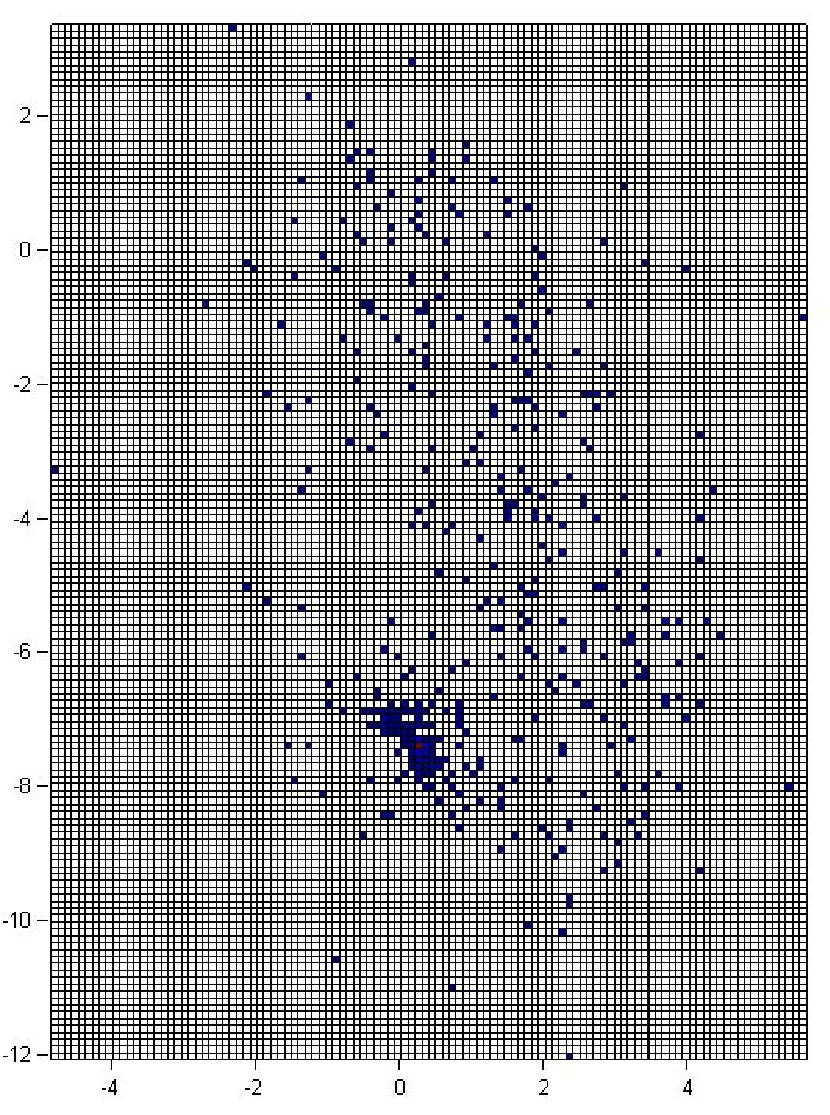
\includegraphics[width=0.45\textwidth]{cmaes-const-noboundaries-dim2-start0_0}}
\quad
\subfloat[z ograniczeniami]{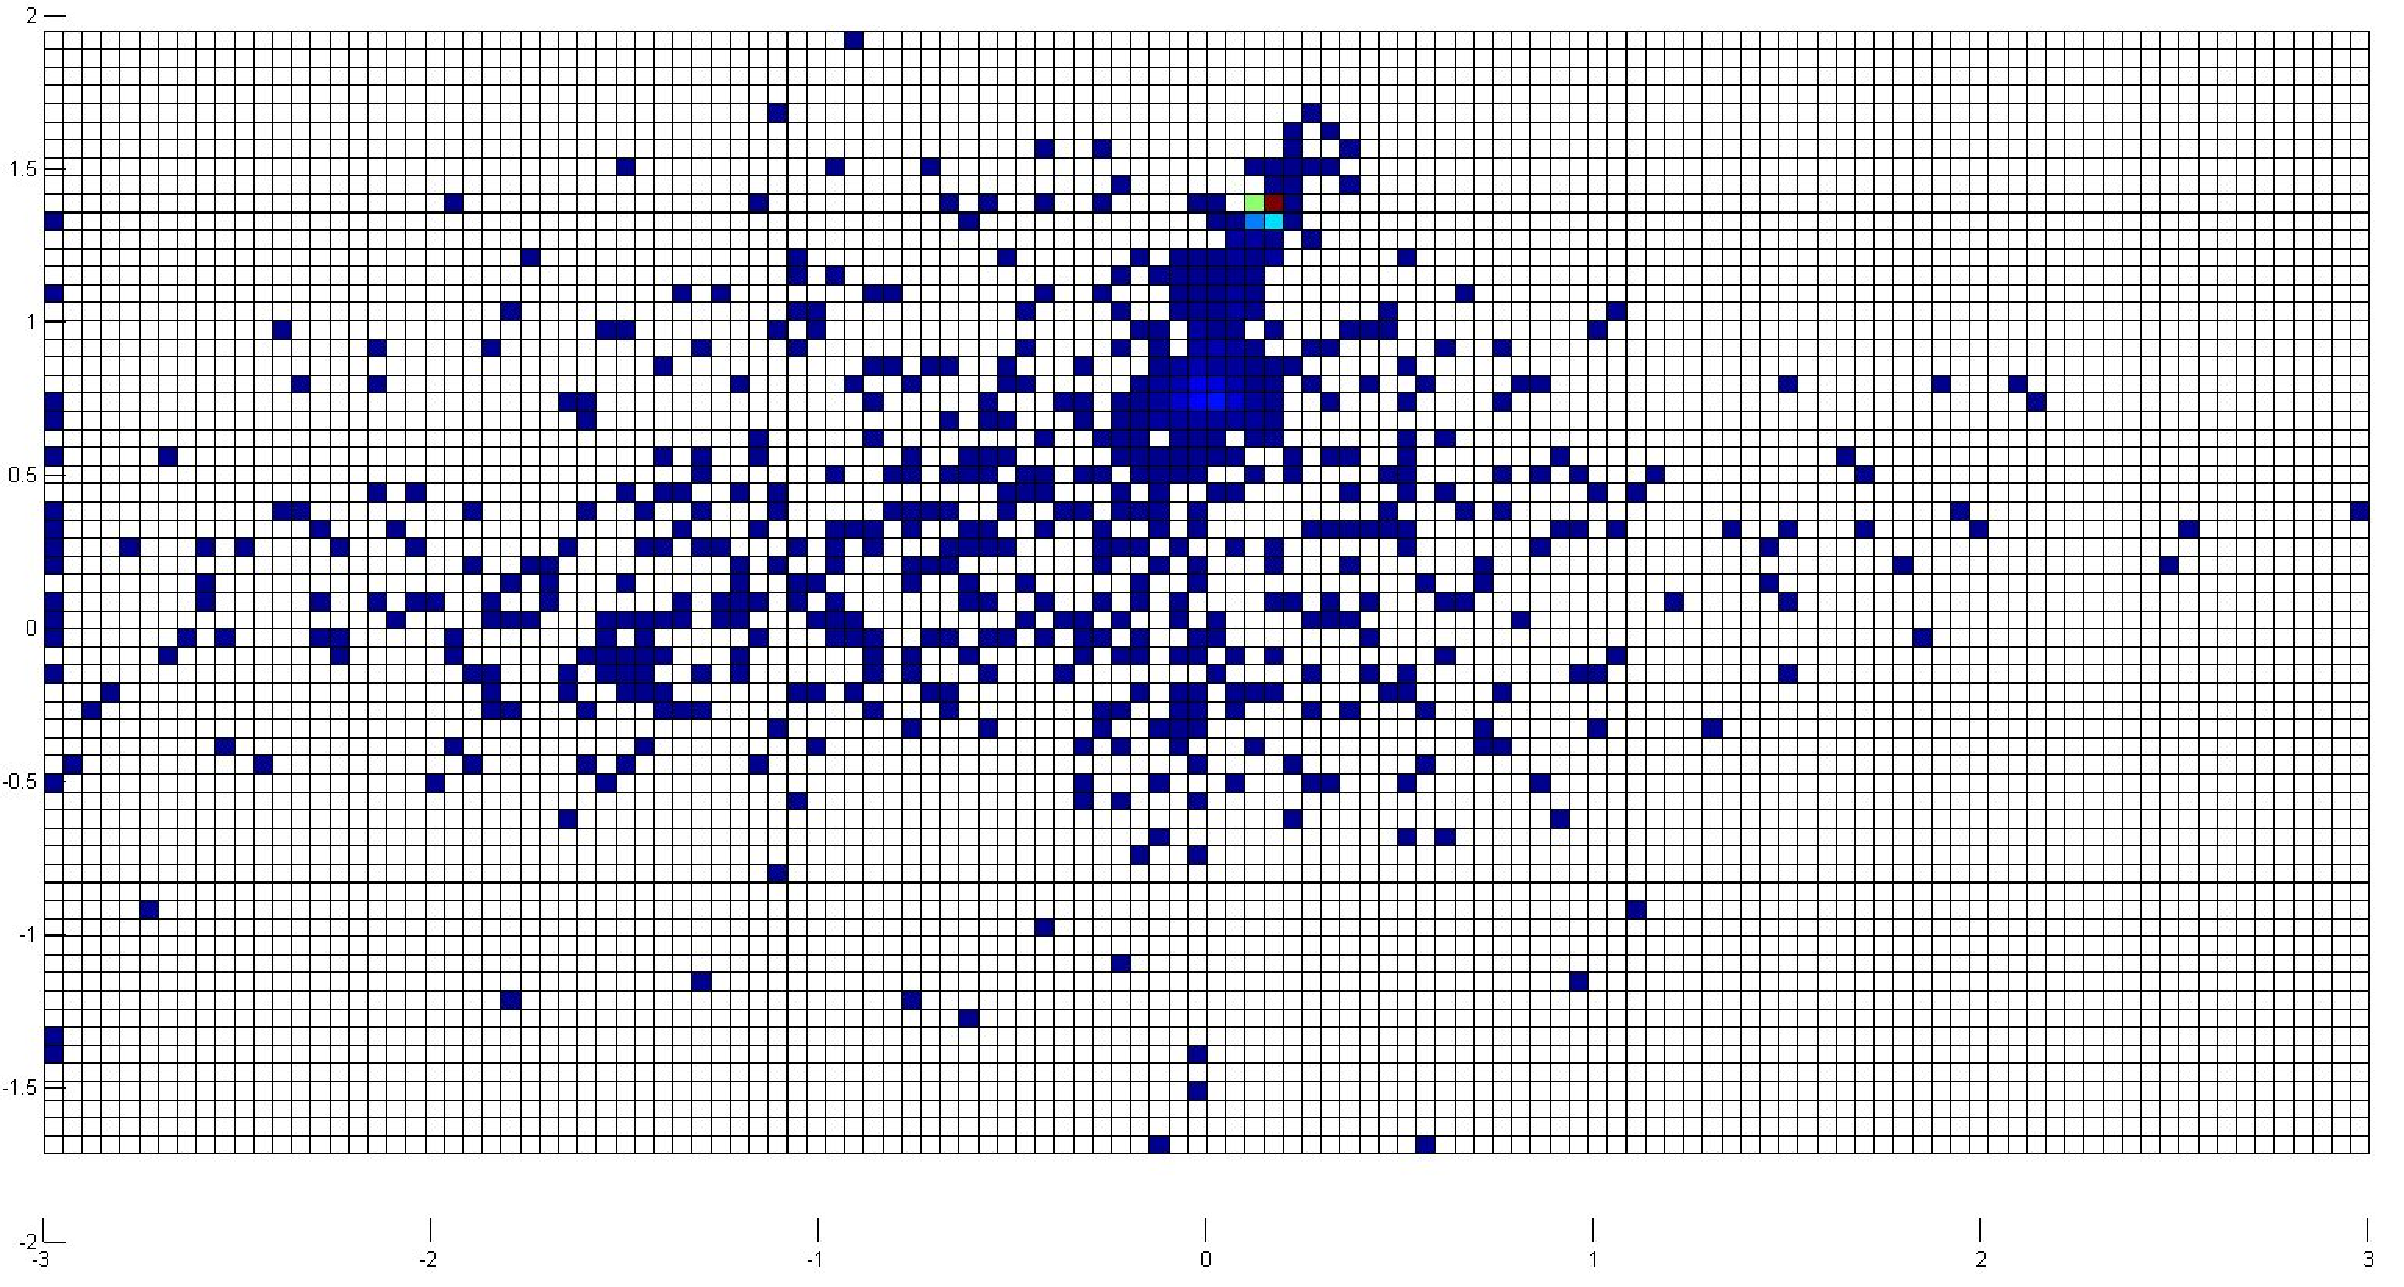
\includegraphics[width=0.45\textwidth]{cmaes-const-boundaries-dim2-start0_0}}
\caption{Histogram punktów; algorytm CMA-ES; funkcja stała; 2 wymiary}
\end{figure}

\subsubsection*{Funkcja losowa}
\hspace{3,4ex}Podobnie jak w przypadku obliczeń dla funkcji stałej, krok algorytmu CMA-ES dla funkcji losowej zmniejszał się dość szybko. Poniższe wykresy, podobnie jak w przypadku testowania funkcji stałej, przedstawiają histogram wystąpień punktów w algorytmie CMA-ES z ograniczeniami oraz bez ograniczenia.

\begin{figure}[H]
\centering
\subfloat[bez ograniczeń]{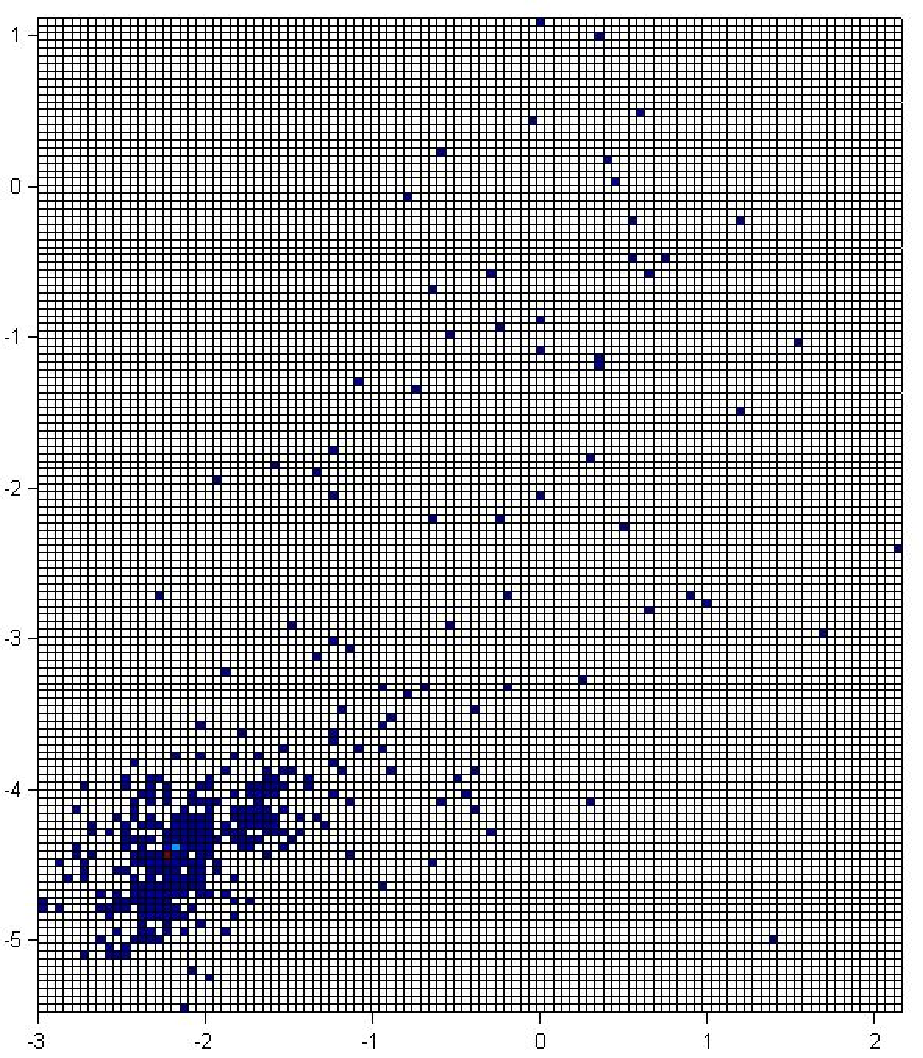
\includegraphics[width=0.45\textwidth]{cmaes-rand-noboundaries-dim2-start0_0}}
\quad
\subfloat[z ograniczeniami]{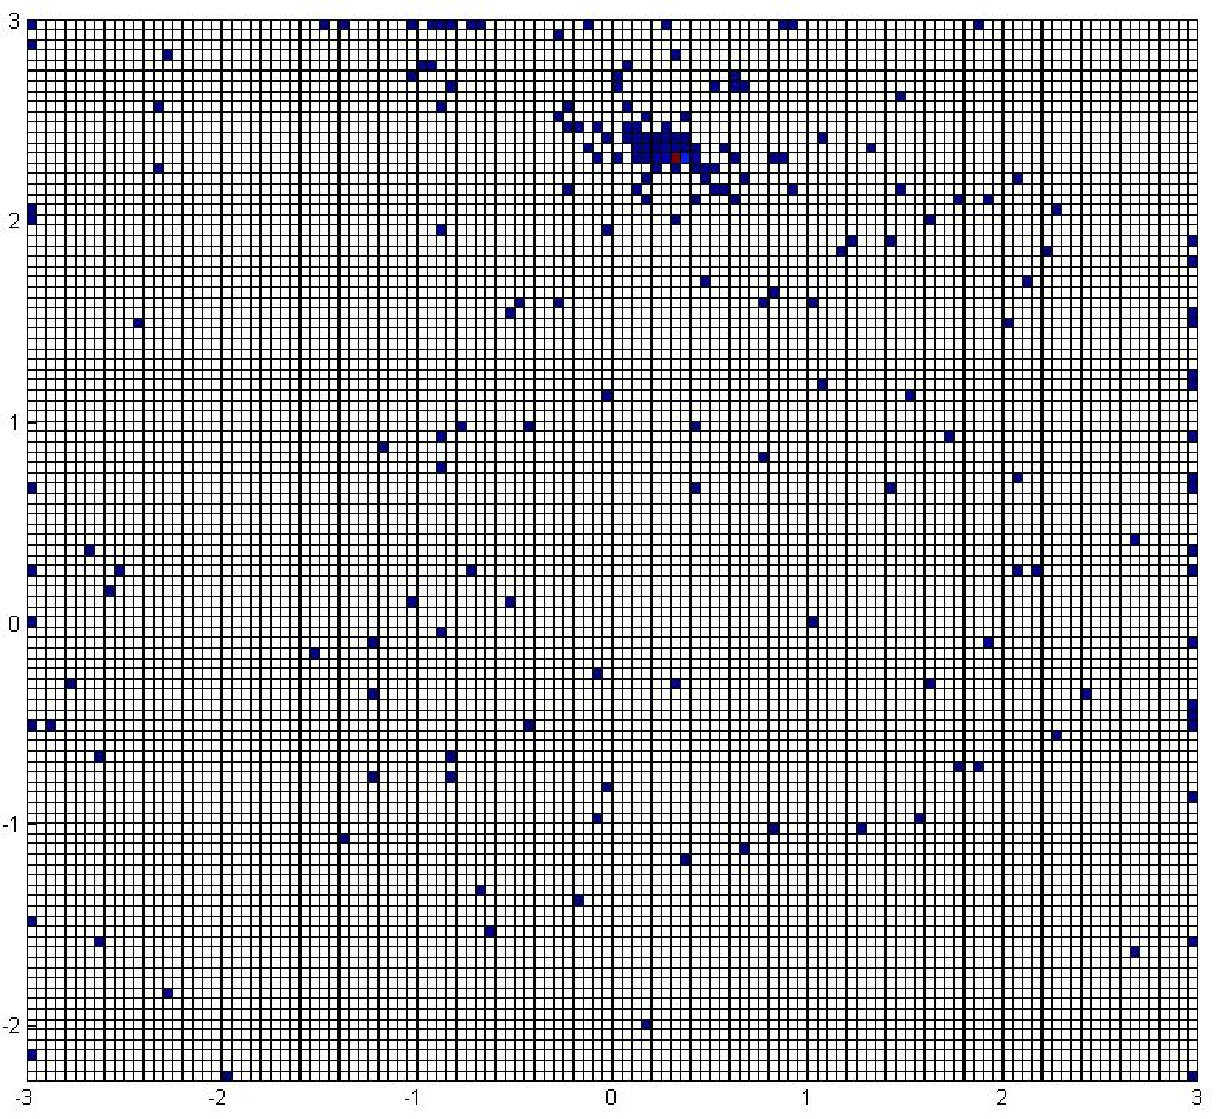
\includegraphics[width=0.45\textwidth]{cmaes-rand-boundaries-dim2-start0_0}}
\caption{Histogram punktów; algorytm CMA-ES; funkcja losowa; 2 wymiary}
\end{figure}

\subsubsection*{Funkcja kwadratowa dwuwymiarowa}
\hspace{3,4ex}Badano funkcję o wzorze $y=x_1^2+x_2^2$. Dla tej funkcji zbiór dopuszczalny zawierał punkty o współrzędnych z zakresu [-0,1;3] na obu wymiarach.Takie ograniczenie zostały wybrane, aby minimum funkcji było blisko narożnika ograniczenia. Takie położenie miało pokazać jak się zachowuje CMA-ES blisko ograniczenia.

Początkowa wartość oczekiwana wynosiła [2;2].Wykres dla tak przygotowanej symulacji znajduje się na rysunku \ref{cmaes:x2} (oś~Z została obcięta do przedziału [0;10]).

\begin{figure}[H]
\centering
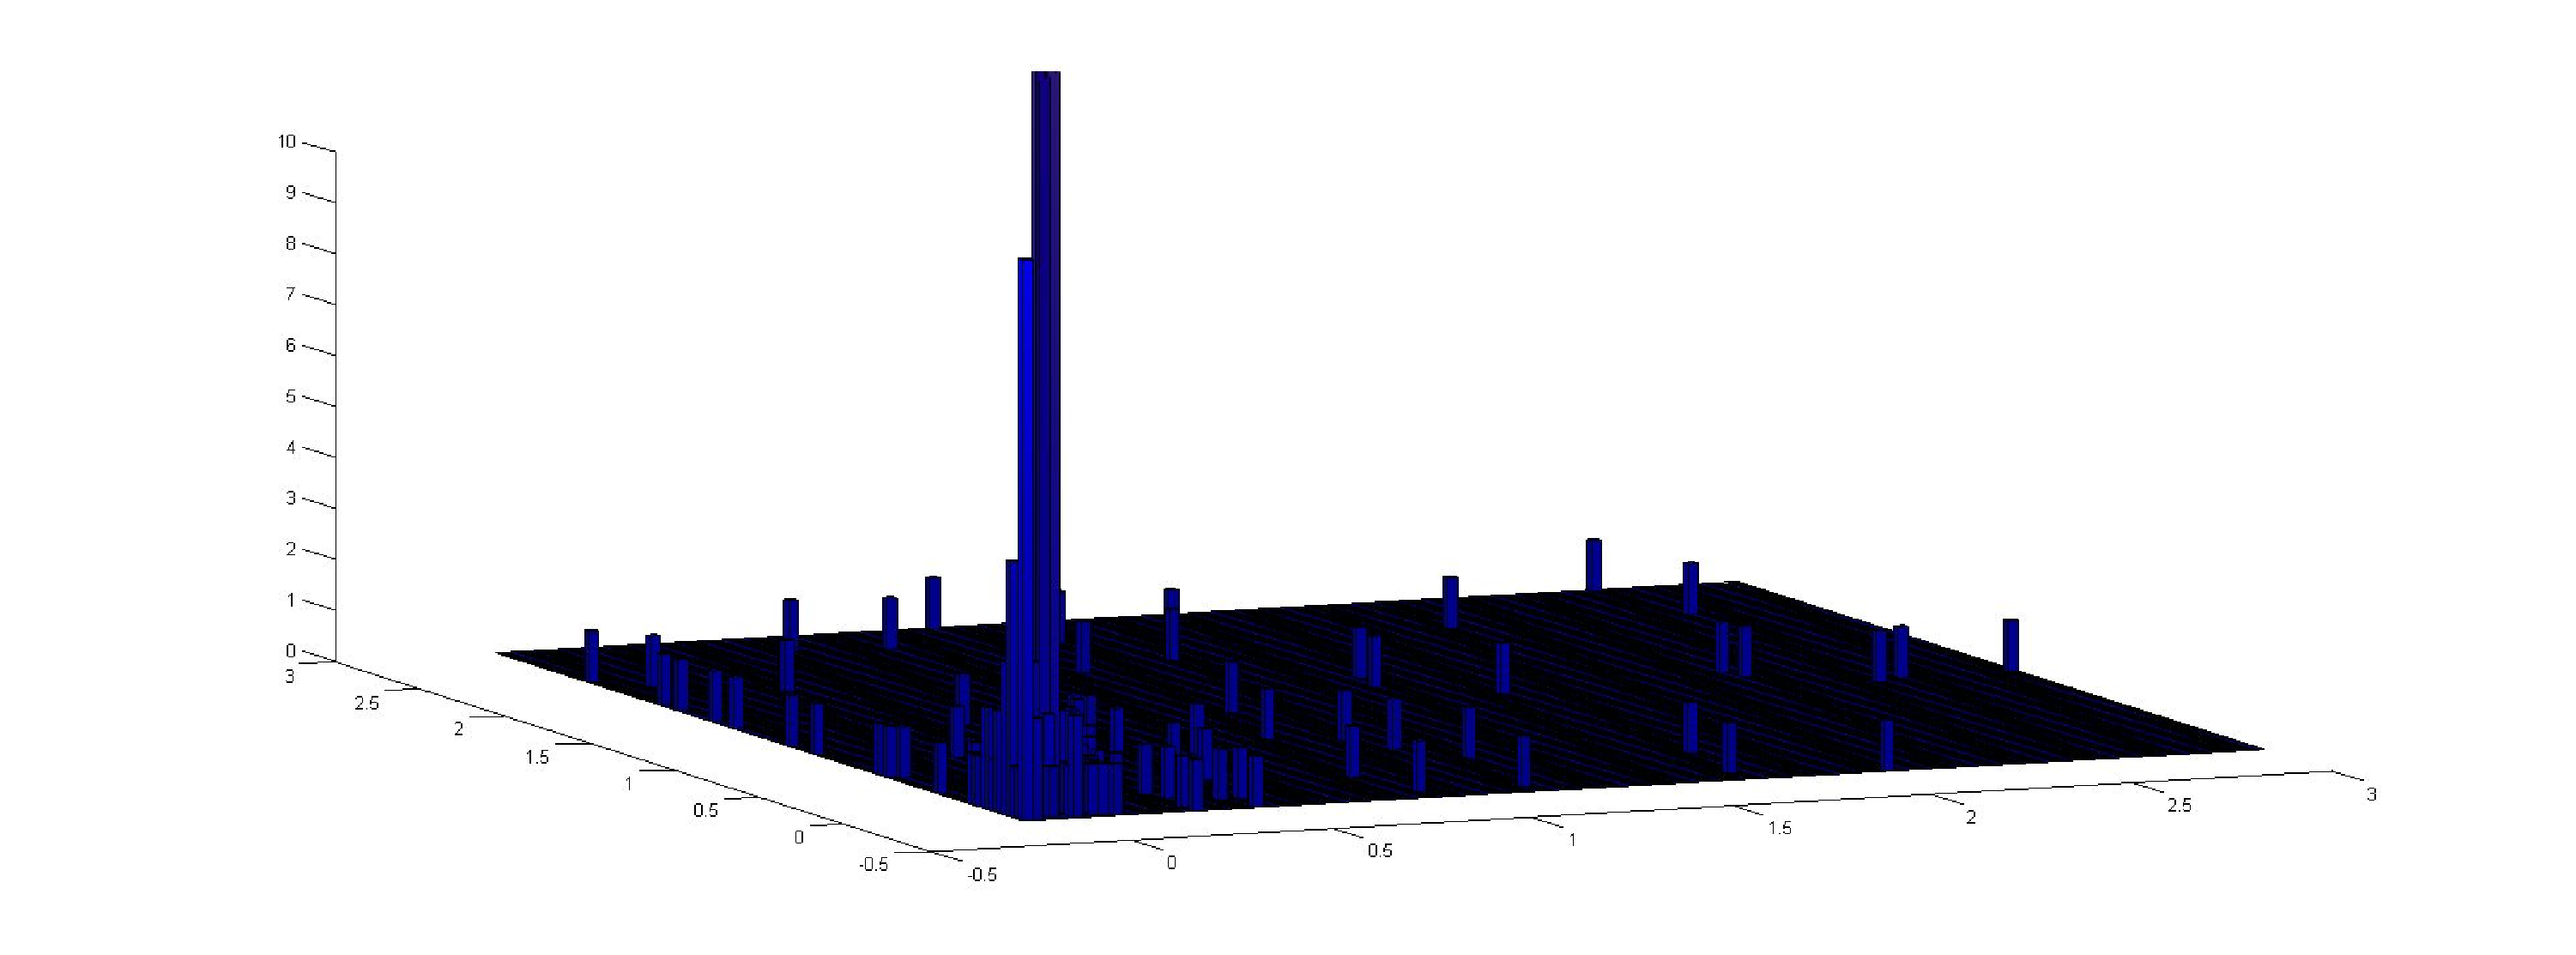
\includegraphics[width=\textwidth]{cmaes-x2dim2-boundaries-v2}
\caption{Histogram punktów; algorytm CMA-ES; funkcja losowa; 2 wymiary}
\label{cmaes:x2}
\end{figure}

\subsubsection{Wnioski}
\hspace{3,4ex}Na wykresach, które przedstawiają histogramy punktów podczas symulacji algorytmu CMA-ES na funkcji losowej i stałej, można zaobserwować tendencję do występowania punktów na ograniczeniach. Było to widoczne również podczas testowania błądzenia przypadkowego. Poza tą własnością, trudno zauważyć inne cechy, ponieważ symulacja zbiega do pewnego punktu - również w przypadku funkcji stałej i losowej. Na podstawie tych wyników trudno cokolwiek powiedzieć o zachowaniu się macierzy kowariancji po dotarciu do ograniczeń kostkowych, ponieważ jest zbyt mało punktów do analizowania.

Autor nie zdecydował się na generowanie wykresów innych metod transformacji rozwiązań, ponieważ nie dałoby to widocznych różnic w wykresach.

\subsection{Porównanie wariantów transformacji rozwiązań}

\subsubsection{Sposób przeprowadzania testów}
\hspace{3,4ex}Celem testów było sprawdzenie, czy wybór techniki uwzględniania ograniczeń w algorytmie CMA-ES wpływa na jakość rozwiązań generowanych przez algorytm.

Najpierw porównano zaimplementowany przez Hansena wariant z rzutowaniem na ograniczenia oraz wariant ewolucji darwinowskiej opisany poniżej. Do kolejnego porównania wybrano 5 wariantów transformacji rozwiązań: rzutowanie na ograniczenie, reinicjacja, odbijanie, zawijanie oraz powtórna generacja.

Dla wszystkich wariantów uruchomiono symulacje algorytmu CMA-ES. W symulacjach wykorzystano funkcje benchmarkowe z konkursu CEC 2013, których dokładny opis znajduje się tutaj \cite{cec}. Ten zestaw został wybrany ze względu na duże zróżnicowanie funkcji oraz implementację w języku MATLAB, z której skorzystano \cite{cec_code}. Algorytm CMA-ES (dla każdego wariantu uwzględniania ograniczeń) uruchomiono po 25 razy dla każdej funkcji benchmarkowej. Do porównań wybrano funkcje z 30 wymiarami. Algorytm CMA-ES dla każdej symulacji zwrócił najlepszy punkt, który znalazł. W ten sposób dla 28 funkcji uzyskano po 25 wartości. Wyniki zostały porównane testem Wilcoxona, aby sprawdzić, czy w istotny sposób się różnią.

\subsubsection*{Ewolucja darwinowska}
\hspace{3,4ex}Do opisania pozostała wspomniana wcześniej ewolucja darwinowska. W tym wariancie punkt nie jest transformowany wewnątrz ograniczenia - jego współrzędne są niezmienne podczas transformacji. Transformacji podlega wartość funkcji. Jest ona taka, jak gdyby punkt został transformowany w ustalony sposób.

W poniższych testach użyto ewolucji darwinowskiej z rzutowaniem na ograniczenie.

\subsubsection*{Metoda konserwatywna}
\hspace{3,4ex}W tych testach nie znalazła się opisywana wcześniej metoda konserwatywna. Wynika to z~faktu, że zakłada ona istnienie powiązań między punktami kolejnych iteracji. W~algorytmie CMA-ES wpływ punktów na kolejną iterację jest pośredni i nie ma tutaj relacji rodzic-potomek.

\subsubsection*{Reinicjacja}
\hspace{3,4ex}W tej metodzie zmieniony został sposób reinicjacji. Zgodnie z rozdziałem \ref{reinicjacja} cały punkt jest przenoszony do pozycji początkowej, gdy którakolwiek z granic jest przekroczona. Takie podejście w algorytmie CMA-ES sprawiało, że algorytm zatrzymywał się w pozycji początkowej, ponieważ losowanie bardzo często zwracało punkt poza ograniczeniami. Zdecydowano się na zmianę tej metody tak, że po przekroczeniu bariery reinicjowane są tylko te wymiary, na których granica została przekroczona. Pozostałe wymiary zostały bez zmian. Obrazuje to poniższy pseudokod:

\begin{Verbatim}[baselinestretch=1.1]
dla każdej współrzędnej i
	jeżeli (lb(i) > x(i)) lub (ub(i) < x(i))
		x(i) = xr(i)
\end{Verbatim}

\subsubsection{Wyniki testów i wnioski}
\hspace{3,4ex}Wyniki zostały zebrane w tabeli. Przedstawia ona porównanie wyników algorytmu CMA-ES z rzutowaniem (wariant podstawowy) do wyników algorytmu CMA-ES z innymi metodami uwzględniania ograniczeń. Wyniki zostały porównane za pomocą testu Wilcoxona. Kolumny są etykietowane numerami funkcji, natomiast wiersze wariantami uwzględniania ograniczeń. Oznaczenia symboli znajdujących się na przecięciach:
\begin{itemize}[noitemsep]
\item --- wariant podstawowy zwrócił statystycznie lepsze wyniki,
\item + wariant podstawowy zwrócił statystycznie gorsze wyniki,
\item . różnice wyników wariantów były nieistotne statystycznie.
\end{itemize}

\begin{table}[H]
\begin{tabular}{|c|c|c|c|c|c|c|c|c|c|c|c|c|c|c|} \hline
Numer funkcji & 1 & 2 & 3 & 4 & 5 & 6 & 7 & 8 & 9 & 10 & 11 & 12 & 13 & 14 \\ \hline
Darwinowska & --- & --- & --- & --- & --- & --- & --- & . & --- & --- & --- & --- & --- & --- \\ \hline \hline
Numer funkcji & 15 & 16 & 17 & 18 & 19 & 20 & 21 & 22 & 23 & 24 & 25 & 26 & 27 & 28 \\ \hline
Darwinowska & --- & . & --- & --- & --- & . & --- & --- & --- & --- & --- & --- & --- & --- \\ \hline
\end{tabular}
\caption{Porównanie testem Wilcoxona wyników zwracanych przez algorytm CMA-ES w wariancie podstawowym z wynikami zwracanymi przez algorytm CMA-ES w wariancie darwinowskim}
\end{table}

\begin{table}[H]
\begin{tabular}{|c|c|c|c|c|c|c|c|c|c|c|c|c|c|c|} \hline
Numer funkcji & 1 & 2 & 3 & 4 & 5 & 6 & 7 & 8 & 9 & 10 & 11 & 12 & 13 & 14 \\ \hline
Reinicjacja & --- & . & . & . & . & . & . & . & + & . & . & . & . & + \\ \hline
Odbijanie & . & . & . & . & . & . & . & . & + & . & . & . & . & . \\ \hline
Zawijanie & . & . & . & . & --- & . & . & . & + & . & . & . & . & + \\ \hline
Powtórna generacja & . & . & . & . & . & . & . & . & + & . & . & . & + & + \\ \hline \hline
Numer funkcji & 15 & 16 & 17 & 18 & 19 & 20 & 21 & 22 & 23 & 24 & 25 & 26 & 27 & 28 \\ \hline
Reinicjacja & . & . & --- & . & . & . & . & + & . & . & --- & . & + & . \\ \hline
Odbijanie & . & . & . & . & . & . & . & . & + & . & . & . & . & . \\ \hline
Zawijanie & + & . & --- & . & . & . & . & + & + & . & --- & . & . & . \\ \hline
Powtórna generacja & + & . & --- & . & . & . & . & + & + & + & . & . & + & . \\ \hline
\end{tabular} 
\caption{Porównanie testem Wilcoxona wyników zwracanych przez algorytm CMA-ES w wariancie podstawowym z wynikami zwracanymi przez algorytm CMA-ES w innych wariantach}
\end{table}

Powyższe tabele pokazują, że wariant ewolucji darwinowskiej zwracał statycznie gorsze wyniki. Nie należy się temu specjalnie dziwić, ponieważ w tej metodzie zmiany wartości funkcji poza ograniczeniami są małe.

W pozostałych porównaniach zazwyczaj różnice są statystycznie nieistotne, natomiast gdy występują, to metoda bazowa częściej zwraca gorsze wyniki. Te różnice są najmniej istotna przy reinicjacji (dla 3 funkcji metoda bazowa zwróciła lepsze wyniki, a dla 4 dla reinicjacji). Nieco tylko inaczej jest w przypadku zawijania (3 - bazowa, 5 - zawijanie). W kontekście tego wyniki odbijania, czyli tylko dla 2 funkcji lepsze rezultaty, wydają się być dość marne. Należy jednak zauważyć, że nie otrzymano rezultatów, które byłyby na korzyść rzutowania.

Zdecydowanie najlepsze rezultaty zwróciła metoda powtórnej generacji - dla 8 funkcji zwróciła lepsze wyniki i tylko dla 1 gorsze.

Metody, które wypadły najlepiej (odbicie i powtórna generacja), sprawiają że średnie przesunięcie punktu nie jest znaczące - można to zauważyć na wykresach wektorów przesunięć w rozdziale \ref{technikiogr}. Można więc wywnioskować, że nie warto zbytnio ingerować w położenie punktu. Na tak postawiony wniosek można podać kontrprzykład z rzutowaniem, które wypadło gorzej. Warto jednak przypomnieć sobie rysunek \ref{bladzenie:rzutowanie2d}, który pokazywał, że w rzutowaniu rozkład prawdopodobieństwa punktów jest bardzo zaburzony, co prowadzi do mniejszej eksploracji przestrzeni. Z tego też względu można upatrywać słabszych wyników rzutowania.

Interesujący jest również fakt, że dla niektórych funkcje (9, 14, 17, 22) porównania wyglądają podobnie. Takie wyniki pokazują, że nie istnieje jeden, najlepszy wariant dla każdej funkcji.


\pagebreak

\section{Podsumowanie}
\hspace{3,4ex}Celem pracy była weryfikacja wpływu uwzględniania ograniczeń kostkowych w algorytmie CMA-ES. Cel ten został zrealizowany poprzez teoretyczne rozważania oraz przeprowadzenie testów.

\subsection{Wnioski}
\hspace{3,4ex}Metoda uwzględnienia ograniczeń kostkowych wpływa na wyniki symulacji algorytmu CMA-ES. Ponadto połączenie pewnych funkcji i ograniczeń daje lepsze rezultaty. Z tych faktów wynika, że czasem warto zadać sobie trud nad wyborem metody uwzględniania ograniczeń, a nawet do tego samego uruchomić kilka symulacji z różnymi metodami.

Kolejnym wnioskiem jest to, że powtórna generacja daje lepsze rezultaty od rzutowania w algorytmie CMA-ES. Należy jednak pamiętać, że powtórna generacja jest bardziej czasochłonne ze względu na konieczność ponownego losowania punktów. Może to być uciążliwe, gdy zależy na szybkości działania, a parametry początkowe sprawiają, że często losowane są punkty niedopuszczalne.

\subsection{Możliwości rozwoju}
\hspace{3,4ex}Przedstawione rozważania mogą posłużyć jako baza do stworzenia nowych wersji algorytmu CMA-ES. Nowy algorytm mógłby w zależności od aktualnych parametrów (położenie wartości oczekiwanej rozkładu, długość kroku, itp.) dobierać odpowiednią metodę uwzględniania ograniczeń.

\pagebreak

\begin{thebibliography}{9}

\bibitem{wyklady}
\emph{Wykłady z algorytmów ewolucyjnych}, Jarosław Arabas, 2004

\bibitem{wilcox}
\emph{The Wilcoxon Signed-Rank Test}, Richard Lowry, \url{http://vassarstats.net/textbook/ch12a.html}

\bibitem{magist}
\emph{Różnicowa implementacja algorytmu CMAES}, Michał Bobowski, 2015

\bibitem{probability}
\emph{An Introduction to Probability Theory and its Applications, Volume II}, William Feller, 1970

\bibitem{cmaes}
\emph{Completely Derandomized Self-Adaptation in Evolution Strategies} w \emph{Evolutionary Computation}, 9(2), pp. 159-195, Nikolaus Hansen, Andreas Ostermeier, 2001

\bibitem{cmaes_code}
\emph{CMA-ES: Evolution Strategy with Covariance Matrix Adaptation for nonlinear function minimization}, Nikolaus Hansen, \url{https://www.lri.fr/~hansen/cmaes\_inmatlab.html}

\bibitem{cmaes_tutorial}
\emph{The CMA evolution strategy: A tutorial. arXiv:1604.00772v1}, Nikolaus Hansen, 2016

\bibitem{cec}
\emph{Problem Definitions and Evaluation Criteria for the CEC 2013 Special Session on Real-Parameter Optimization}, J. J. Liang, B. Y. Qu, P. N. Suganthan, Alfredo G. Hernández-Díaz, 2013

\bibitem{cec_code}
\emph{CEC13 Test Function Suite }, Jane Jing Liang, \url{http://web.mysites.ntu.edu.sg/epnsugan/PublicSite/Shared%20Documents/CEC2013/cec13matlab.zip}

\bibitem{zast}
\emph{Algorytmy ewolucyjne i ich zastosowania} w \emph{Zeszyty naukowe}, 1/2006, pp. 81-92, Ewa Figielska, 2006

\bibitem{lcmaes}
\emph{Reducing the Space-Time Complexity of the CMA-ES}, James N. Knight, Monte Lunacek, 2007

\bibitem{bbob}
\emph{Comparing Results of 31 Algorithms from the Black-Box Optimization Benchmarking BBOB-2009}, N. Hansen, A. Auger, R. Ros, S. Finck, P. Posik, 2010

\end{thebibliography}

\makestatement

\end{document}
